%!TeX spellcheck = en-UK, el-GR
%this tex file is compatible with lualatex compiler because of the fontspec package usage
\documentclass[11pt]{report}
% geometry package is used to size the paper
\usepackage[a4paper,width=170mm,top=25mm,bottom=25mm,headheight=15pt]{geometry}
% natbib package is used to format the bibliography
\usepackage[round]{natbib}
% a bibliography styler
\bibliographystyle{unsrtnat}
% Bibliography in table of contents
\usepackage[nottoc]{tocbibind}
% fancyhdr is used to format the headers of the paper
\usepackage{fancyhdr}
% the header styler
\pagestyle{fancy}
% fncychap is used to format the chapter titles
\usepackage[Rejne]{fncychap}
% fontspec package is used to choose the Arial font
\usepackage{fontspec}
% set font to Arial
\setmainfont[Ligatures=TeX]{Arial}
% hyperref package is used to reference pages, chapters, figures etc in the paper
\usepackage[hidelinks,linktocpage]{hyperref}
% ragged2e package is used for the \justified format
\usepackage{ragged2e}
% make space between each line 1.5
\renewcommand{\baselinestretch}{1.5}
% graphicx package is used to input photos in the paper
\usepackage{graphicx}
%bfloat package is used to size tables
\usepackage{float}
% amsmath packages is used for the math formulas in the paper
\usepackage{amsmath}
% diagbox package is used to format the first row/column header in one cell
\usepackage{diagbox}
% color package is used for text coloring
\usepackage{color}
% use multiple languages
\usepackage[greek,english]{babel}

% set the path to find the images for the graphicx package
\graphicspath{ {images/} }

\title{
	{\large
	 University of the Aegean\\
	 School of Engineering\\
	 Department of Financial and Management Engineering}\\
	 \vfill
	{
\includegraphics{cover/cover.eps}}\\
	\vfill
	{«Recursive Nearest Neighbors Methods in Recommender Systems»}\\
}
\author{Stylianos Tsesmetzis\\ {\small Supervisor: Nicholas Ampazis}}
\date{{Chios,} 31/10/2017}
\begin{document}
\pagenumbering{Roman}
\maketitle
\addcontentsline{toc}{chapter}{Cover}

\clearpage

\chapter*{Abstract}
\addcontentsline{toc}{chapter}{Abstract}
% !TeX root = ../main.tex

A recommender system is a software that analyses the behavior of its users and
tries to recommend products relevant to their interests. Through the years a lot
of different recommendation techniques have been introduced. One of them is called
neighborhood-based collaborative filtering. This technique is one of the
earliest developed in the context of recommender systems. As in every
technique, collaborative filtering has its own advantages and disadvantages.
Its main disadvantage is that it needs lots of user ratings
before it can form enough relations to understand users interests and
recommend products.

In this thesis, a recursive approach will be introduced that tries to
overcome the limitations of the conventional neighborhood-based collaborative
filtering and generate more predictions, resulting in
better recommendations. As a case study the recursive nearest neighbors algorithm
was evaluated in the Epinions data set, with a variety of similarity metrics
such as Cosine Similarity, Pearson Correlation Coefficient, etc and with
different error metrics RMSE, MAE, MAUE, RMSUE in order to test its performance.
The results showed that there has been a significant increase in the number of rating
predictions and at the same time the inclusion of these new rating predictions
in the error metrics resulted in only a slight increase in the total error of the model.\\\\
\justify
\textbf{Keywords:} Recommender Systems, Collaborative Filtering,
                   Nearest Neighbors, Recursive method, \\Epinions dataset


\begin{otherlanguage}{greek}
\chapter*{\abstractname}
\addcontentsline{toc}{chapter}{\abstractname}
% !TeX spellcheck = el-GR
% !TeX root = ../main.tex

Ένα σύστημα συστάσεων είναι ένα λογισμικό που αναλύει τη
συμπεριφορά των χρηστών του και προσπαθεί να συστήσει προϊόντα
σχετικά με τα ενδιαφέροντα τους. Κατά το πέρασμα των χρόνων
εισήχθησαν πολλές διαφορετικές τεχνικές σύστασης. Μια από αυτές ονομάζεται
συνεργατικό φιλτράρισμα βάσει γειτονιάς. Αυτή η τεχνική είναι μία
από τις πρώτες που αναπτύχθηκαν στο πλαίσιο των συστημάτων
συστάσεων. Όπως σε κάθε τεχνική, έτσι και το συνεργατικό φιλτράρισμα έχει τα
δικά του πλεονεκτήματα και μειονεκτήματα. Το κύριο μειονέκτημα του
είναι ότι χρειάζεται πολλές βαθμολογίες από τους χρήστες
πριν να μπορέσει να δημιουργήσει αρκετές διασυνδέσεις
για να κατανοήσει τα ενδιαφέροντα των χρηστών και να προτείνει
προϊόντα.

Σε αυτή τη διπλωματική εργασία θα εισαχθεί μια αναδρομική προσέγγιση που
θα προσπαθήσει να ξεπεράσει τους περιορισμούς του συνηθισμένου
γειτονικού φιλτραρίσματος και να δημιουργήσει
περισσότερες προβλέψεις, που θα έχει ως αποτέλεσμα καλύτερες συστάσεις.
Ως μελέτη περίπτωσης, ο αλγόριθμος αναδρομικών πλησιέστερων γειτόνων
αξιολογήθηκε στο σύνολο δεδομένων Epinions με μια ποικιλία μετρήσεων ομοιότητας
όπως Ομοιότητα συνημιτόνου, Συντελεστής Συσχέτισης Pearson κ.λπ. και με διαφορετικές
μετρικές σφαλμάτων RMSE, MAE, MAUE, RMSUE με σκοπό να δοκιμασθεί η απόδοσή του.
Τα αποτελέσματα έδειξαν ότι υπήρξε σημαντική αύξηση του αριθμού των προβλέψεων αξιολόγησης
και ταυτόχρονα η συμπερίληψη αυτών των νέων προβλέψεων αξιολόγησης
στις μετρικές σφάλματος έδειξε ότι το συνολικό σφάλμα του μοντέλου αυξήθηκε ελάχιστα.\\
\justify
\textbf{Λέξεις Κλειδιά:} Συστήματα Υποδείξεων, Συνεργατικό Φιλτράρισμα,
Πλησιέστεροι Γείτονες, \\Αναδρομική Μέθοδος, σύνολο δεδομένων Epinions

\end{otherlanguage}

\chapter*{Dedication}
\addcontentsline{toc}{chapter}{Dedication}
\begin{center}
	To my parents,\\
	Stergios and Stergiani\\
	and my siblings,\\
	Stratos and Maria.
\end{center}

\chapter*{Acknowledgements}
\addcontentsline{toc}{chapter}{Acknowledgements}
% !TeX root = ../main.tex

First of all I would like to thank my supervisors Nicholas Ampazis and
Dimosthenis Drivaliaris for their intense support in all my questions and difficulties
that occurred during the realization of my thesis. Furthermore, I would like
to explicitly express my appreciation for the useful advices provided by
Flwra Sakketoy, the experiment hours and the time she dedicated in reviewing my thesis.
Last but not least, I would like to express my gratitude to my best friends
Andreas Mavridis and Alexandros Athanasoulis for their moral and research support
during the realization of my thesis which was the core part that kept me going
until its completion.


\tableofcontents\addcontentsline{toc}{chapter}{\contentsname}
\listoffigures
\listoftables
\cleardoublepage\pagenumbering{arabic}
\chapter{Introduction}
\label{chap:1}
% !TeX root = ../main.tex

\section{Recommender systems overview}
A Recommender System (RS) is defined as a software that analyses the behavior
and activities of users, for example as in an online retail platform like
Amazon \citep{amazon}, and provides them with content relevant to their
interests \citep{Ricci, Jannach}. In RSs the term "user" means the customer
that interacts with the online platform. To find content that seems relevant
to the users an RS uses algorithms that help it make decisions on what
items to suggest \citep{Ricci}. The term "item" is used to denote anything
that the RS recommends to a user. Recommender systems can be used in many domains.
A list of the most popular recommender platforms is shown in \autoref{table:Recommenders Examples}:

\begin{table}[H]
\centering
\caption{Examples of products recommended by various real-world recommender
         systems \citep{Aggarwal}}
\label{table:Recommenders Examples}
\begin{tabular}{ |c|c| }
\hline
\textbf{System} & \textbf{Product Goal}\\
\hline
Amazon.com & Books and other products\\
\hline
Netflix & DVDs, Streaming Video\\
\hline
Jester & Jokes\\
\hline
GroupLens & News\\
\hline
MovieLens & Movies\\
\hline
last.fm & Music\\
\hline
Google News & News\\
\hline
Google Search & Advertisements\\
\hline
Facebook & Friends, Advertisements\\
\hline
Pandora & Music\\
\hline
YouTube & Online videos\\
\hline
Tripadvisor & Travel products\\
\hline
IMDb & Movies\\
\hline
\end{tabular}
\end{table}

In many of these RSs, a rating system is used in order to provide item
recommendations to their users. A rating system is a feedback method
(e.g. number of stars) typically in the interval [1 - 5] which indicates the
level of satisfaction about an item they have bought \citep{Aggarwal}.
These ratings are stored in a matrix, namely the "ratings matrix", where
each row represents a user's ratings to each item and each column represents
an item's ratings by each user.
After the users buy a book, hear a song or watch a movie they can rate it so
other users know how much they like or dislike a particular item.

After many years of research, a lot of algorithms have been introduced to
increase the efficiency of the recommender systems. These algorithms can be
broadly assigned to the following techniques:

\begin{itemize}
	\item \textbf{Collaborative Filtering (CF):} Recommender systems using CF
    techniques are based on the assumption that users who used to like similar
    items in the past will continue to like similar items in the future
    \citep{Jannach}. The basic source of information for CF is the rating
    system. It uses this information for two reasons.
    The first is to use the known ratings in the system to predict the
    missing ratings. The second is to use the predicted ratings to
    recommend the most suitable items for each user in terms of relevance.
    CF can be separated in two distinct types, Memory-based and Model-based:\\
	\begin{enumerate}
    	\item \textbf{Memory-Based:} The motivation for this name comes from
        the fact that this method keeps the rating database in memory and uses
        it directly for generating the recommendations \citep{Jannach}.
    	This method is also called neighborhood-based because it uses the
        known ratings to find similarities between users or items in order to
        generate predictions.
    	When the similarities refer to users the method it is called user-based
        collaborative filtering. When they refer to items it is called
        item-based collaborative filtering.
    	In user-based collaborative filtering the ratings predictions
        are derived from filtering the most similar users to the active user
        (the user that the RS is calculating the predictions for) that
        have also interacted with the item the prediction is calculated for.
        Then, with respect to the similarity of those users and their ratings
        on the specific item, an aggregation is calculated as the prediction
        of the rating for this item that the active user would give.

    	\item \textbf{Model-Based:} In model-based methods, machine learning
    	and data mining methods are used in the context of predictive models.
        In cases where the model is parameterized, the parameters of this
        model are learned within the context of an optimization framework.
        Some examples of such model-based methods include decision trees,
        rule-based models, Bayesian methods and latent factor models.
        Many of these methods, such as latent factor models, have a high
        level of coverage even for sparse ratings matrices \citep{Aggarwal}.
        The term "sparse ratings matrix" means that many of these ratings are missing
        from the ratings matrix,
        as it is unlikely that every user has rated every item.
	\end{enumerate}
	\item \textbf{Content-based Recommender System:} Another way to extract
    information about what a user might be interested in and provide
    relevant recommendations is by observing the content this user spends more
    time on. Instead of trying to match the patterns of different users ratings
    like in CF, this method focuses on what attributes
    it can extract from the items the user is looking at. The brand name in
    a shirt, the genre or actors in a movie, the actual text of a book are
    all very strong indicators that the user is looking for something
    specific. Similarities in this case are formed from the common attributes
    of the existing items in the platform. A content-based approach is
    also very useful when a new user enters the platform where CF suffers
    from the cold start problem (The recommender system is not aware of
    any of the new user's preferences) \citep{Aggarwal}.
	\item \textbf{Knowledge-based Recommender Systems:} This type of RS differs from
    the aforementioned techniques as it does not rely neither on user or item
    collaborations nor on item attributes to generate recommendations. Instead,
    this RS interactively tries to guide the user through the choices, that they would
    make most sense to them at a particular time, by forming similarities between the
    user's requirements and the available items \citep{Jannach}. The reason for such an RS can be
    understood for example when a user wants to buy a house. The preferences of a user evolve,
    for example family or lifestyle situations would led the user to different decisions at
    that particular time. If a CF recommendation was given instead, it might match the user
    with houses of irrelevant specifications.
	\item \textbf{Hybrid Recommender Systems:} These types of RSs are based on the
    combination of the above mentioned techniques. A hybrid system combining e.g.
    techniques A and B tries to use the advantages of A to fix the
    disadvantages of B. \citep{Ricci}
\end{itemize}

In summary, every recommender system's goal is to increase the profit of the
company that is using it. To better define this goal in technical parts,
it was split in more meaningful subgoals \citep{Aggarwal}.
These subgoals are:

\begin{enumerate}
  \item \textbf{Relevance}: In order to drive users to buy the company's items, the
  recommendations must be relevant to users' preferences.
  \item \textbf{Novelty}: Blockbusters in every domain are easy to be found.
  A recommender's job is to surprise the user with items that this user would
  like but in the most cases has never heard of. As \citep{Fleder} argues,
  recommending popular items over and over may bore the user resulting in
  sales decrease.
  \item \textbf{Serendipity (pleasant surprise)}: Recommending items for which there
  is a high chance that the user would like it is one thing. Recommending items
  almost irrelevant to that user but suspecting the user would love this is a
  serendipity. Sometimes recommender systems try to broaden users' choices
  by selecting alternatives to the users' tastes. In other words they try to
  avoid overspecialization \citep{Jannach}.
  \item \textbf{Recommendation diversity}: When the recommender system knows
  e.g. that a user likes books about Recommender Systems from a specific author,
  recommending only these books and from only this author wouldn't mean that the
  user is interested in buying more of those. For example, a book about
  Linear Algebra or Programming might also catch this user's interest.
\end{enumerate}

\section{Purpose}
In this thesis we will focus on the neighborhood-based CF and how to overcome some
of its drawbacks. This method's drawbacks are mainly:
\begin{enumerate}
    \item \textbf{Scale:} New users and items enter the recommendation system everyday.
    That means that the system has to form similarities between the new user and the
    already existing users or the new item and the already existing items and make
    predictions. For a video streaming company like Netflix \citep{netflix}, with over
    100 million users and more than 10 thousand movies and TV shows, regularly updating
    similarities between users would use unreasonable computing resources. That
    would also mean recalculating over 10 billion rating predictions.
    \item \textbf{Sparse data:} It is very unlikely that every user has rated
    every item. That means that a lot of ratings are missing from the ratings matrix.
    That also means that it is impossible to form similarities between all users
    or all items and if, e.g. a user does not have rated items in common with many
    other users, it will lead to the RS not being able to make predictions for
    that user for many items.
    \item \textbf{Cold start:} The RS has no information on how a user rates or
    an item is being rated on users and items that have just entered the system. Therefore,
    until users rate items or items receive ratings by users, the RS has to
    ignore them because it is not able to form any similarities.
\end{enumerate}
The first objective in this thesis is to explore ways to generate more rating
predictions to overcome the drawback of sparse data. For that purpose we will use the
Epinions dataset \citep{Massa}. It contains 40163 users and 139738 items and
664824 ratings. The sparsity percentage which is given by the formula
$sparsity\ percentage = \frac{total\ possible\ ratings - current\ ratings}{total\ possible\ ratings}$
, where\\$total\ possible\ ratings = total\ users*total\ items$, is 0,99988154. This means that a
typical collaborative filtering method like the K-Nearest Neighbors(KNN) algorithm
\citep{schafer2007collaborative} that will be discussed in \autoref{chap:2}
would fail to find a lot of similarities between users or items and generate
predictions. The second objective is to keep a relatively low error on
rating predictions with a new neighborhood-based CF algorithm that will be later defined.

\section{Approach}
In this thesis a neighborhood-based CF algorithm will be proposed in \autoref{chap:3}
that is called Recursive K-Nearest Neighbors. This method tries to overcome the limitations of
the memory-based collaborative filtering method mentioned above.
The algorithm is a novel approach, in the sense that is able of predicting ratings that
normal KNN algorithm would fail due to lack of
similarities. This algorithm is tested with a variety of similarity metrics that will
be discussed in \autoref{chap:2} and the accuracy for each metric is evaluated
with four different cost functions, namely Root Mean Squared Error(RMSE), Mean Absolute
Error(MAE), Root Mean Squared User Error(RMSUE) and Mean Absolute User
Error(MAUE) in \autoref{chap:4}.


\chapter{Neighborhood-based CF}
\label{chap:2}
% !TeX root = ../main.tex

\section{Introduction}
The earliest algorithms developed in recommender systems were
neighborhood-based collaborative filtering algorithms. These algorithms
utilize the similarities between either of users or items, based on the ratings.
The data in a recommender system can be presented as a matrix called the ratings
matrix($\mathcal{R}$).
\begin{table}[H]
\centering
\begin{tabular}{ |c|c|c|c|c| }
\hline
\diagbox{$User$}{$Item$} & \textbf{$Item_1$} & \textbf{$Item_2$} & \textbf{$Item_3$} & \textbf{$Item_4$} \\
\hline
\textbf{$User_1$} & 5 & 2 & \textbf{?} & 3 \\
\hline
\textbf{$User_2$} & 1 & \textbf{?} & 4 & 2 \\
\hline
\textbf{$User_3$} & \textbf{?}  & 3 & 5 & 4 \\
\hline
\textbf{$User_4$} & 5 & 2 & 3 &  \textbf{?} \\
\hline
\textbf{$User_5$} & 1 & \textbf{?}  & 2 & 4 \\
\hline
\textbf{$User_6$} & 3 & 5 & \textbf{?}  & 3 \\
\hline
\textbf{$User_7$} & 3 & 1 & \textbf{?}  & 5 \\
\hline
\end{tabular}
\caption{Ratings Matrix}
\label{table:Ratings Matrix}
\end{table}

\justify
The rows of the matrix represent users($\mathcal{U}$) and the
columns represent items($\mathcal{I}$). A rating($r$) is a number in this case an integer in
the range [1 - 5] that a user has given to an item, where 1 means that
the users totally disliked the item and 5 that the user totally liked the item. The missing ratings are those
that the users haven't reviewed yet and also where the rating predictions apply.
The known ratings are used for the similarity computations and therefore for
the rating predictions. There are two types of neighborhood-based algorithms:
\begin{itemize}
	\item \textbf{User-based CF:}  This type utilizes the ratings matrix
	row-wise meaning the recommender system is trying to find similar patterns
	between users. Given the ratings matrix, to predict the rating that
	$User_4$ would give to $Item_4$ first it would try to find users
	that have rated $Item_4$ and out of these users to select those
	(also called nearest neighbors) who have liked similar items with $User_4$
	in the past. Then based on the most similar nearest neighbors to $User_4$
	a prediction would be computed as an aggregation of the target user's nearest neighbors
	ratings. This method assumes two things. The first one is that if users
	had similar interests in the past they will have similar interests in the future.
	The second assumption is that user preferences remain stable and
	consistent over time. \citep{Jannach}

	\item \textbf{Item-based CF:} This type utilizes the ratings matrix
	column-wise and it is trying to find patterns between the items. Again
	from the ratings matrix, to predict the rating that $User_4$ would give to
	$Item_4$ it would try to find other items, that this user has rated. The
	rating prediction would  be an aggregation of the ratings of the most similar
	items between those and $Item_4$. Item-based CF is considered a more viable approach in
	real cases for two reasons. The first reason is that the items are usually far
	less than the users	in the system. This reduces both the computation
	time and storage needed for the similarities. The second reason is that
	users tend to rate a small proportion of items, which distorts the
	user similarities because of the sparseness. Instead, each item accumulates more
	ratings, as items are less than users, which makes item-based
	similarities more reliable.\citep{sarwar2001item}
\end{itemize}
The main advantages of the neighborhood-based algorithms\citep{Ricci} are:
\begin{itemize}
	\item \textbf{Simplicity:} To implement a neighborhood-based algorithm
	the only factor that is considered is the ratings in the matrix in order
	to find similarities.
	\item \textbf{Justifiability:} It is very clear how the rating
	predictions were computed and why it makes sense from the data as the
	similarities that gave these predictions can be provided to the users, so
	as to justify their relevance.
	\item \textbf{Efficiency:} The training cost in neighbor-based methods
	consists only of the similarity pre-computations between users or items
	which can be computed offline in the ratings matrix which is much cheaper than
	most model-based training. Offline learning means that the system
	will not adapt immediately to any change. Instead it must recompute
	the similarities from scratch. Moreover, storing only the nearest neighbors
	in memory requires only a little use of RAM, instead of storing every user
	which could form a similarity with the active user.
	\item \textbf{Stability:} In large scale recommenders systems, typically in
	item-based approach, it is observed that the addition of users, items and ratings slightly
	affect the decisions of the system after item similarities have been computed.
	That means that the RS would not need further re-training to make better recommendations.
	Also when new items enter the system, they can be trained solely without affecting other items'
	existing similarities.
\end{itemize}

As discussed in the previous chapter, neighborhood-based algorithms suffer from the sparsity of
the ratings matrix. When the similarities are calculated from
only a few common ratings between, e.g. two items, this often leads to
an ambiguous similarity score that can produce spurious predictions.
Another symptom of sparseness is that sometimes no similarities between
items or users can be found and this inability leaves those items or users
without neighbors. Thus, without neighbors they won't participate in
the rating prediction process which means that the RS won't be able to provide
recommendations for those entities.

In \autoref{sec:2.2} different similarity metrics will be discussed.
In \autoref{sec:2.3} The KNN algorithm will be explained and a full example will be
demonstrated for further clarification.

\section{Similarity Metrics}\label{sec:2.2}
The most important part in a neighborhood-based CF approach is the computation of
the similarities which, as we discussed above, can be user-based or item-based.
Below, different similarity metrics will be mentioned. Some of them are widely known metrics
in the literature. These are Cosine Similarity, Pearson Correlation Coefficient,
Adjusted Cosine Similarity, Mean Absolute Difference, Mean Squared Difference and
Jaccard Coefficient. The rest of them are modifications
of the original metrics that we introduce and do not exist in the literature.
These are the Modified Cosine Similarity, Modified Adjusted Cosine Similarity,
Modified Pearson Correlation Coefficient 1 and Modified Pearson Correlation Coefficient 2.
Some of the widely known similarity metrics have been introduced as a user-based approach
and others as item-based. In this thesis we will define each similarity metric both for
user-based and item-based. Also we will assume that the values of the ratings matrix
consist of integers in the interval [1, 5] in order to define the interval for
each similarity metric.
\subsection{Mathematical Notation}
For consistency over the similarity metrics formulas that will be defined next,
a global mathematical notation is used for the rest of this section.
Uppercase $\mathcal{I}$ is used to denote the set of items in the system.
The notation $\mathcal{I}_u$ is the set of items that have been rated by
user $u$, $\mathcal{I}_v$ is the set of items that have been rated by
user $v$ and $\mathcal{I}_{uv}$ is $\mathcal{I}_u \cap \mathcal{I}_v$ that is the set of items that users $u$ and $v$ have
rated in common.
Similarly, uppercase $\mathcal{U}$ is used to denote the set of users in the system.
$\mathcal{U}_i$ is the set of users that have rated
item $i$, $\mathcal{U}_j$ is the set of users that have rated
item $j$ and $\mathcal{U}_{ij}$ is $\mathcal{U}_i \cap \mathcal{U}_j$ that is the set of users that have rated both
items $i$ and $j$. The notation $\mathopen|\mathcal{I}_{u}\mathclose|$ denotes
the number of items user $u$ has rated, $\mathopen|\mathcal{I}_{v}\mathclose|$
denotes the number of items user $v$ has rated, and $\mathopen|\mathcal{I}_{uv}\mathclose|$
is the number of items that users $u$ and $v$ have rated in common. Likewise,
$\mathopen|\mathcal{U}_{i}\mathclose|$ denotes the number of users that have
rated item $i$, $\mathopen|\mathcal{U}_{j}\mathclose|$ denotes the number of users that have rated
item $j$, and $\mathopen|\mathcal{U}_{ij}\mathclose|$ is the number of users that
have both rated items $i$ annd $j$.
$r_{ui}$ is the rating that user $u$ gave to item $i$ and
$r_{vi}$ the rating that user $v$ gave to item $i$.
$r_{iu}$ is the rating item $i$ received from user $u$ and
$r_{ju}$ the rating item $j$ received from user $u$.

\subsection{Cosine similarity}
Cosine similarity is a metric that measures the cosine of the angle that two vectors form.
This metric can take any value in the interval [-1, 1], but specifically for our
own case where the ratings matrix is defined in the interval [1, 5], this
metric is defined in the interval [0, 1].\\\\
User-based cosine similarity between users $u$ and $v$ is defined as:
\begin{equation}\label{eq:cosine}
    cos(u,v) = \frac{\sum_{i \in \mathcal{I}_{uv}}r_{ui}r_{vi}}
		    {\sqrt{\sum_{i \in \mathcal{I}_{u}}r_{ui}^2}
		     \sqrt{\sum_{i \in \mathcal{I}_{v}}r_{vi}^2}}
\end{equation}
The largest the similarity value the higher is chance that these users rate by the same way.
A zero similarity score indicates that $u$ and $v$ have no items in common and therefore
they have no similarity.\\\\
From \autoref{table:Ratings Matrix}, the cosine similarity
between $User_1$ and $User_3$ would thus be computed as follows:
\begin{align*}
cos(User_1,User_3) = \frac{2*3 + 3*4}
						{\sqrt{5^2 + 2^2 + 3^2} * \sqrt{3^2 + 5^2 + 4^2}} = 0.4129
\end{align*}
Similarly, instead of using the row vectors to calculate the similarity between users,
column vectors can be used to calculate the similarity between item pairs.\\\\
Item-based cosine similarity between items $i$ and $j$ is defined as:
\begin{equation}
    cos(i,j) = \frac{\sum_{u \in \mathcal{U}_{ij}}r_{iu}r_{ju}}
		    {\sqrt{\sum_{u \in \mathcal{U}_{i}}r_{iu}^2}
		     \sqrt{\sum_{u \in \mathcal{U}_{j}}r_{ju}^2}}
\end{equation}
Again from \autoref{table:Ratings Matrix}, the cosine similarity
between $Item_2$ and $Item_3$ would thus be computed as follows:
\begin{align*}
cos(Item_2,Item_3) = \frac{3*5 + 2*3}
						{\sqrt{2^2 + 3^2 + 2^2 + 5^2 + 1^2} * \sqrt{4^2 + 5^2 + 3^2 + 2^2}} = 0.4358
\end{align*}
\subsection{Modified Cosine Similarity}
Modified cosine similarity differs from the standard cosine similarity in the
sense that the computations in the denominator apply only to the common items
between $u$ and $v$.
Its values are defined in the interval [0, 1].\\\\
User-based modified cosine similarity between users $u$ and $v$ is defined as:
\begin{equation}\label{eq:modified_cosine}
    MC(u,v) = \frac{\sum_{i \in \mathcal{I}_{uv}}r_{ui}r_{vi}}
		   {\sqrt{\sum_{i \in \mathcal{I}_{uv}}r_{ui}^2}
                    \sqrt{\sum_{i \in \mathcal{I}_{uv}}r_{vi}^2}}
\end{equation}
From \autoref{table:Ratings Matrix}, MC
between $User_1$ and $User_3$ would thus be computed as follows:
\begin{align*}
MC(User_1,User_3) = \frac{2*3 + 3*4}
					   {\sqrt{2^2 + 3^2} * \sqrt{3^2 + 4^2}} = 0.9984
\end{align*}
We can reverse the above formula in order to calculate the similarities
in terms of items.\\
Item-based modified cosine similarity between items $i$ and $j$ is defined as:
\begin{equation}
    MC(i,j) = \frac{\sum_{u \in \mathcal{U}_{ij}}r_{iu}r_{ju}}
   {\sqrt{\sum_{u \in \mathcal{U}_{ij}}r_{iu}^2}
            \sqrt{\sum_{u \in \mathcal{U}_{ij}}r_{ju}^2}}
\end{equation}
From \autoref{table:Ratings Matrix}, MC
between $Item_2$ and $Item_3$ would thus be computed as follows:
\begin{align*}
MC(Item_2,Item_3) = \frac{3*5 + 2*3}
						{\sqrt{3^2 + 2^2} * \sqrt{5^2 + 3^2}} = 0.9988
\end{align*}
\subsection{Adjusted Cosine Similarity}
Adjusted cosine similarity was originally created as an
item-based approach. The reason for that was because each item vector consists of
users who have different rating behaviors and cosine similarity did not
take into account these disparities. That means that a user could use the
rating 3 for items that really liked and 1 for items that really disliked while
another user could give a 5 rating to items that really liked and 1 to them that really
disliked. Adjusted cosine similarity is computed by looking into the co-rated items
($\mathcal{U}_{ij}$) only. It normalizes each user's rating behavior by
subtracting the corresponding user's mean value \citep{sarwar2001item}.
Adjusted cosine similarity values are defined in the interval [-1, 1].
The value -1 means perfect dissimilarity between two items while the value 1 means
perfect similarity. The zero value means there is no similarity between these items.\\\\
Item-based adjusted cosine similarity between items $i$ and $j$ is defined as:
\begin{equation}\label{eq:adjusted_cosine}
    \begin{split}
    &AC(i,j) = \frac{\sum_{u \in \mathcal{U}_{ij}}(r_{iu}-\bar{r_{u}})(r_{ju}-\bar{r_{u}})}
		    {\sqrt{\sum_{u \in \mathcal{U}_{ij}}(r_{iu}-\bar{r_{u}})^2}
                     \sqrt{\sum_{u \in \mathcal{U}_{ij}}(r_{ju}-\bar{r_{u}})^2}} \\\\
    &\bar{r_{u}} = \frac{\sum_{i \in \mathcal{I}_u}r_{ui}}
 		        {\mathopen|\mathcal{I}_u\mathclose|}
    \end{split}
\end{equation}
where,
\begin{itemize}
	\item[] $\bar{r_u}$ is the mean value of user $u$ for each $u \in \mathcal{U}_{ij}$
\end{itemize}
From \autoref{table:Ratings Matrix}, AC
between $Item_2$ and $Item_3$ would thus be computed as follows:
\begin{align*}
	\begin{split}
		&\bar{r}_{User_3} = \frac{3 + 5 + 4}{3} = 4\\
		&\bar{r}_{User_4} = \frac{5 + 2 + 3}{3} = 3.33
	\end{split}
\end{align*}
$$AC(Item_2,Item_3) = \frac{(3 - 4)*(5 - 4) + (2 - 3.33)*(3 - 3.33)}
						 {\sqrt{(3 - 4)^2 + (2 - 3.33)^2}*
						  \sqrt{(5 - 4)^2 + (3 - 3.33)^2}} = −0.3202$$
The result $-0.3202$ means that $Item_2$ and $Item_3$ are somewhat dissimilar.\\\\
We could use the same reasoning adjusted cosine was build on,
to look at this formula from a user-based perspective. That is, if an item's
lowest rating is 3 and its highest rating is 5, that means that it is treated
differently than an item that its lowest rating is 1 and the highest 4.
Therefore, we could have each co-rated item, by two users, mean centered by the corresponding item
and calculate a user-based adjusted cosine similarity.\\\\
User-based adjusted cosine similarity between users $u$ and $v$ is defined as:
\begin{equation}
\begin{split}
    &AC(u,v) = \frac{\sum_{i \in \mathcal{I}_{uv}}(r_{ui}-\bar{r_{i}})(r_{vi}-\bar{r_{i}})}
		    {\sqrt{\sum_{i \in \mathcal{I}_{uv}}(r_{ui}-\bar{r_{i}})^2}
                     \sqrt{\sum_{i \in \mathcal{I}_{uv}}(r_{vi}-\bar{r_{i}})^2}} \\\\
    &\bar{r_{i}} = \frac{\sum_{u \in \mathcal{U}_i}r_{iu}}
 		        {\mathopen|\mathcal{U}_i\mathclose|}
\end{split}
\end{equation}
where,
\begin{itemize}
	\item[] $\bar{r_i}$ is the mean value of item $i$ for each $i \in \mathcal{I}_{uv}$
\end{itemize}
From \autoref{table:Ratings Matrix}, AC
between $User_1$ and $User_3$ would thus be computed as follows:
\begin{align*}
	\begin{split}
		&\bar{r}_{Item_2} = \frac{2 + 3 + 2 + 5 + 1}{5} = 2.6\\
		&\bar{r}_{Item_4} = \frac{3 + 2 + 4 + 4 + 3 + 5}{6} = 3.5
	\end{split}
\end{align*}
$$AC(User_1,User_3) = \frac{(2 - 2.6)*(3 - 2.6) + (3 - 3.5)*(4 - 3.5)}
						 {\sqrt{(2 - 2.6)^2 + (3 - 3.5)^2}*
						  \sqrt{(3 - 2.6)^2 + (4 - 3.5)^2}} = −0.9798$$
$User_1$ and $User_3$ are almost perfectly dissimilar.
\subsection{Modified Adjusted Cosine Similarity}
A modification to adjusted cosine similarity that we implemented was to
use every user corresponding to $i$ and $j$ instead of using
only the users that have rated both items in the denominator. Its values are also in the interval [-1, 1].\\\\
Item-based modified adjusted cosine similarity between items $i$ and $j$ is defined as:
\begin{equation}
\begin{split}
&MAC(i,j) = \frac{\sum_{u \in \mathcal{U}_{ij}}(r_{iu}-\bar{r_{u}})(r_{ju}-\bar{r_{u}})}
				 {\sqrt{\sum_{u \in \mathcal{U}_{i}}(r_{iu}-\bar{r_{u}})^2}
				  \sqrt{\sum_{u \in \mathcal{U}_{j}}(r_{ju}-\bar{r_{u}})^2}} \\\\
&\bar{r_{u}} = \frac{\sum_{i \in \mathcal{I}_u}r_{ui}}
					{\mathopen|\mathcal{I}_u\mathclose|}
\end{split}
\end{equation}
where,
\begin{itemize}
	\item[] $\bar{r_u}$ is the mean value of user $u$ for each $u \in \mathcal{U}_{ij}$ in the numerator
	\item[] $\bar{r_u}$ is the mean value of user $u$ for each $u \in \mathcal{U}_{i}$ and $u \in \mathcal{U}_{j}$ respectively in the denominator
\end{itemize}
From \autoref{table:Ratings Matrix}, MAC
between $Item_2$ and $Item_3$ would thus be computed as follows:
\footnotesize
\begin{align*}
	\begin{split}
		&\bar{r}_{User_1} = \frac{5 + 2 + 3}{3} = 3.33\\
		&\bar{r}_{User_2} = \frac{1 + 4 + 2}{3} = 2.33\\
		&\bar{r}_{User_3} = \frac{3 + 5 + 4}{3} = 4\\
		&\bar{r}_{User_4} = \frac{5 + 2 + 3}{3} = 3.33\\
		&\bar{r}_{User_5} = \frac{1 + 2 + 4}{3} = 2.33\\
		&\bar{r}_{User_6} = \frac{3 + 5 + 3}{3} = 3.66\\
		&\bar{r}_{User_7} = \frac{3 + 1 + 5}{3} = 3\\\\
&MAC(Item_2,Item_3) = \\&\frac{(3 - 4)*(5 - 4) + (2 - 3.33)*(3 - 3.33)}
						 {\sqrt{(2 - 3.33)^2 + (3 - 4)^2 + (2 - 3.33)^2 + (5 - 3.66)^2 + (1 - 3)^2}*
						  \sqrt{(4 - 2.33)^2 + (5 - 4)^2 + (3 - 3.33)^2 + (2 - 2.33)^2}} \\&= −0,0872
  \end{split}
\end{align*}
\normalsize
Compared to item-based AC the item-based MAC between $Item_2$ and $Item_3$ still generates
a negative similarity but it is very close to zero this time as it takes into account each
item's vector length.\\\\
As previously mentioned a user-based approach can also be implemented.\\
User-based modified adjusted cosine similarity between users $u$ and $v$ is defined as:
\begin{equation}\label{eq:modified_adjusted_cosine}
\begin{split}
    &MAC(u,v) = \frac{\sum_{i \in \mathcal{I}_{uv}}(r_{ui}-\bar{r_{i}})(r_{vi}-\bar{r_{i}})}
                     {\sqrt{\sum_{i \in \mathcal{I}_{u}}(r_{ui}-\bar{r_{i}})^2}
                      \sqrt{\sum_{i \in \mathcal{I}_{v}}(r_{vi}-\bar{r_{i}})^2}} \\\\
    &\bar{r_{i}} = \frac{\sum_{u \in \mathcal{U}_i}r_{iu}}
                        {\mathopen|\mathcal{U}_i\mathclose|}
\end{split}
\end{equation}
where,
\begin{itemize}
	\item[] $\bar{r_i}$ is the mean value of user $u$ for each $u \in \mathcal{I}_{uv}$ in the numerator
	\item[] $\bar{r_i}$ is the mean value of user $u$ for each $u \in \mathcal{I}_{u}$ and $u \in \mathcal{I}_{v}$ respectively in the denominator
\end{itemize}
From \autoref{table:Ratings Matrix}, MAC
between $User_1$ and $User_3$ would thus be computed as follows:
\begin{align*}
	\begin{split}
		&\bar{r}_{Item_1} = 3\\
		&\bar{r}_{Item_2}  = 2.6\\
		&\bar{r}_{Item_3} = 3.5\\
		&\bar{r}_{Item_4} = 3.5\\\\
MAC(User_1,User_3) &= \frac{(2 - 2.6)*(3 - 2.6) + (3 - 3.5)*(4 - 3.5)}
						 {\sqrt{(5 - 3)^2 + (2 - 2.6)^2 + (3 - 3.5)^2}*
						  \sqrt{(3 - 2.6)^2 + (5 - 3.5)^2 + (4 - 3.5)^2}} \\&= −0.1399
  \end{split}
\end{align*}
Compared to user-based AC, the user-based MAC between $User_1$ and $User_3$ still generates
a negative similarity but it is far weaker than AC's as it takes into account the length of
each user's vector.
\subsection{Pearson Correlation Coefficient}
Users do not always rate in the same way. One user might never use a rating of 5
for items that really likes.
Another user might never rate an item below 3 for items that really dislikes.
A third user might only use a rating of 4 despite of how much he liked an item.
This means is that most of the users have a particularity in their
ratings. Due to this user behavior, it is difficult to understand the similarity
based on the actual rating. The Pearson correlation coefficient
computes the linear correlation between two users, to alleviate this problem. Linear correlation is
defined as the proportion of dependence between two variables X and Y.
Regarding the similarity between two users, the Pearson correlation coefficient can also be
thought of as the covariance between two users A and B divided by the standard deviation of
$User_A$ multiplied by the standard deviation of $User_B$.\\\\
User-based Pearson correlation coefficient between users $u$ and $v$ is defined as:
\begin{equation}\label{eq:pearson}
\begin{split}
    &PCC(u,v) = \frac{\sum_{i \in \mathcal{I}_{uv}}(r_{ui}-\bar{r_{u}})(r_{vi}-\bar{r_{v}})}
                     {\sqrt{\sum_{i \in \mathcal{I}_{uv}}(r_{ui}-\bar{r_{u}})^2}
                      \sqrt{\sum_{i \in \mathcal{I}_{uv}}(r_{vi}-\bar{r_{v}})^2}} \\\\
    &\bar{r_{u}} = \frac{\sum_{i \in \mathcal{I}_u}r_{ui}}
                        {\mathopen|\mathcal{I}_u\mathclose|}\\
    &\bar{r_{v}} = \frac{\sum_{i \in \mathcal{I}_v}r_{vi}}
                        {\mathopen|\mathcal{I}_v\mathclose|}
\end{split}
\end{equation}
where,
\begin{itemize}
	\item[] $\bar{r_u}$ is the mean value of user $u$
	\item[] $\bar{r_v}$ is the mean value of user $v$
\end{itemize}
The PCC varies between -1 and 1 and based on its value two objects inspected for correlation can
be classified as:
\begin{itemize}
	\item Positively correlated, when $PCC > 0$
	\item Negatively correlated, when $PCC < 0$
	\item Uncorrelated,  when $PCC = 0$
\end{itemize}
From \autoref{table:Ratings Matrix}, PCC
between $User_1$ and $User_3$ would thus be computed as follows:
\begin{align*}
	\begin{split}
		&\bar{r}_{User_1} = 3.33\\
		&\bar{r}_{User_3} = 4\\\\
		PCC(User_1,User_3) &= \frac{(2 - 3.33) * (3 - 4) + (3 - 3.33) * (4 - 4)}
								  {\sqrt{(2 - 3.33)^2 + (3 - 3.33)^2} *
								   \sqrt{(3 - 4)^2 + (4 - 4)^2}} = 0.9705
	\end{split}
\end{align*}
Thus $User_1$ and $User_3$ have a strong positive correlation.\\\\
PCC was initially used as a user-based approach\citep{shardanand1995social} but we will
reverse it for item-based computations in order to measure the correlation between the items.\\\\
Item-based Pearson correlation coefficient between items $i$ and $j$ is defined as:
\begin{equation}
	\begin{split}
	&PCC(i,j) = \frac{\sum_{u \in \mathcal{U}_{ij}}(r_{iu}-\bar{r_{i}})(r_{ju}-\bar{r_{j}})}
					 {\sqrt{\sum_{u \in \mathcal{U}_{ij}}(r_{iu}-\bar{r_{i}})^2}
					  \sqrt{\sum_{u \in \mathcal{U}_{ij}}(r_{ju}-\bar{r_{j}})^2}} \\\\
	&\bar{r_{i}} = \frac{\sum_{u \in \mathcal{U}_i}r_{iu}}
						{\mathopen|\mathcal{U}_i\mathclose|}\\
	&\bar{r_{j}} = \frac{\sum_{u \in \mathcal{U}_j}r_{ju}}
						{\mathopen|\mathcal{U}_j\mathclose|}
\end{split}
\end{equation}
where,
\begin{itemize}
	\item[] $\bar{r_i}$ is the mean value of item $i$
	\item[] $\bar{r_j}$ is the mean value of item $j$
\end{itemize}
From \autoref{table:Ratings Matrix}, PCC
between $Item_2$ and $Item_3$ would thus be computed as follows:
\begin{align*}
	\begin{split}
		&\bar{r}_{Item_2} = 2.6\\
		&\bar{r}_{Item_3} = 3.5\\\\
		PCC(Item_2,Item_3) &= \frac{(3 - 2.6) * (5 - 3.5) + (2 - 2.6) * (3 - 3.5)}
								  {\sqrt{(3 - 2.6)^2 + (2 - 2.6)^2} *
								   \sqrt{(5 - 3.5)^2 + (3 - 3.5)^2}} = 0.7893
	\end{split}
\end{align*}
Thus $Item_2$ and $Item_3$ have a strong positive correlation.
\subsection{Modified Pearson Correlation Coefficient 1}
The first modification to PCC that we implemented was to average only the ratings that
two users have in common. Its values are in the interval [-1, 1].\\\\
User-based modified Pearson correlation coefficient 1 between users $u$ and $v$ is defined as:
\begin{equation}\label{eq:pearson_1}
\begin{split}
    &MPCC1(u,v) = \frac{\sum_{i \in \mathcal{I}_{uv}}(r_{ui}-\tilde{r_{u}})(r_{vi}-\tilde{r_{v}})}
                       {\sqrt{\sum_{i \in \mathcal{I}_{uv}}(r_{ui}-\tilde{r_{u}})^2}
                        \sqrt{\sum_{i \in \mathcal{I}_{uv}}(r_{vi}-\tilde{r_{v}})^2}} \\\\
    &\tilde{r_{u}} = \frac{\sum_{i \in \mathcal{I}_{uv}}r_{ui}}
                          {\mathopen|\mathcal{I}_{uv}\mathclose|}\\
    &\tilde{r_{v}} = \frac{\sum_{i \in \mathcal{I}_{uv}}r_{vi}}
                          {\mathopen|\mathcal{I}_{uv}\mathclose|}
\end{split}
\end{equation}
where,
\begin{itemize}
	\item[] $\tilde{r_u}$ is the mean value of user $u$ using only the co-rated items with user $v$
	\item[] $\tilde{r_v}$ is the mean value of user $v$ using only the co-rated items with user $u$
\end{itemize}
From \autoref{table:Ratings Matrix}, MPCC1
between $User_1$ and $User_3$ would thus be computed as follows:
\begin{align*}
	\begin{split}
		&\tilde{r}_{User_1} = \frac{2 + 3}{2} = 2.5\\
		&\tilde{r}_{User_3} = \frac{3 + 4}{2} = 3.5\\\\
		MPCC1(User_1,User_3) &= \frac{(2 - 2.5) * (3 - 3.5) + (3 - 2.5) * (4 - 3.5)}
								  {\sqrt{(2 - 2.5)^2 + (3 - 2.5)^2} *
								   \sqrt{(3 - 3.5)^2 + (4 - 3.5)^2}} = 1
	\end{split}
\end{align*}
Compared to user-based PCC, the user-based MPCC1 between $User_1$ and $User_3$
using the modified mean values yields a perfect correlation.\\\\
Item-based modified Pearson correlation coefficient 1 between items $i$ and $j$ is defined as:
\begin{equation}
	\begin{split}
	&MPCC1(i,j) = \frac{\sum_{u \in \mathcal{U}_{ij}}(r_{iu}-\tilde{r_{i}})(r_{ju}-\tilde{r_{j}})}
					 {\sqrt{\sum_{u \in \mathcal{U}_{ij}}(r_{iu}-\tilde{r_{i}})^2}
					  \sqrt{\sum_{u \in \mathcal{U}_{ij}}(r_{ju}-\tilde{r_{j}})^2}} \\\\
	&\tilde{r_{i}} = \frac{\sum_{u \in \mathcal{U}_{ij}}r_{iu}}
						{\mathopen|\mathcal{U}_{ij}\mathclose|}\\
	&\tilde{r_{j}} = \frac{\sum_{u \in \mathcal{U}_{ij}}r_{ju}}
						{\mathopen|\mathcal{U}_{ij}\mathclose|}
\end{split}
\end{equation}
where,
\begin{itemize}
	\item[] $\tilde{r_i}$ is the mean value of item $i$ using only the common user ratings with item $j$
	\item[] $\tilde{r_j}$ is the mean value of item $j$ using only the common user ratings with item $i$
\end{itemize}
From \autoref{table:Ratings Matrix}, MPCC1
between $Item_2$ and $Item_3$ would thus be computed as follows:
\begin{align*}
	\begin{split}
		&\tilde{r}_{Item_2} = \frac{3 + 2}{2} = 2.5\\
		&\tilde{r}_{Item_3} = \frac{5 + 3}{2} = 4\\\\
		MPCC1(Item_2,Item_3) &= \frac{(3 - 2,5) * (5 - 4) + (2 - 2,5) * (3 - 4)}
								  {\sqrt{(3 - 2,5)^2 + (2 - 2,5)^2} *
								   \sqrt{(5 - 4)^2 + (3 - 4)^2}} = 1
	\end{split}
\end{align*}
Compared to item-based PCC, item-based MPCC1 between $Item_2$ and $Item_3$
using the modified mean values yields a perfect correlation.
\subsection{Modified Pearson Correlation Coefficient 2}
The second modification to PCC is to change the denominator
in a sense that it includes all the items corresponding to $u$ and $v$ respectively.
Its values are also in the interval [-1, 1].\\\\
User-based modified Pearson correlation coefficient 2 between users $u$ and $v$ is defined as:
\begin{equation}\label{eq:pearson_2}
\begin{split}
    &MPCC2(u,v) = \frac{\sum_{i \in \mathcal{I}_{uv}}(r_{ui}-\bar{r_{u}})(r_{vi}-\bar{r_{v}})}
                       {\sqrt{\sum_{i \in \mathcal{I}_{u}}(r_{ui}-\bar{r_{u}})^2}
                        \sqrt{\sum_{i \in \mathcal{I}_{v}}(r_{vi}-\bar{r_{v}})^2}} \\\\
    &\bar{r_{u}} = \frac{\sum_{i \in \mathcal{I}_u}r_{ui}}
                        {\mathopen|\mathcal{I}_u\mathclose|}\\
    &\bar{r_{v}} = \frac{\sum_{i \in \mathcal{I}_v}r_{vi}}
                        {\mathopen|\mathcal{I}_v\mathclose|}
\end{split}
\end{equation}
where,
\begin{itemize}
	\item[] $\bar{r_u}$ is the mean value of user $u$
	\item[] $\bar{r_v}$ is the mean value of user $v$
\end{itemize}
From \autoref{table:Ratings Matrix}, MPCC2
between $User_1$ and $User_3$ would thus be computed as follows:
\begin{align*}
	\begin{split}
		&\bar{r}_{User_1} = 3.33\\
		&\bar{r}_{User_3} = 4\\\\
		MPCC2(User_1,User_3) &= \frac{(2 - 3.33) * (3 - 4) + (3 - 3.33) * (4 - 4)}
								  {\sqrt{(5 - 3.33)^2 + (2 - 3.33)^2 + (3 - 3.33)^2} *
								   \sqrt{(3 - 4)^2 + (5 - 4)^2 + (4 - 4)^2}} = 0.4353
	\end{split}
\end{align*}
Compared to user-based PCC, the user-based MPCC2 between $User_1$ and $User_3$
retained a positive correlation but it has significantly decreased as it now
takes into account the mean centered length of each user's vector.\\\\
Item-based modified Pearson correlation coefficient 2 between items $i$ and $j$ is defined as:
\begin{equation}
	\begin{split}
	&MPCC2(i,j) = \frac{\sum_{u \in \mathcal{U}_{ij}}(r_{iu}-\bar{r_{i}})(r_{ju}-\bar{r_{j}})}
					 {\sqrt{\sum_{u \in \mathcal{U}_{i}}(r_{iu}-\bar{r_{i}})^2}
					  \sqrt{\sum_{u \in \mathcal{U}_{j}}(r_{ju}-\bar{r_{j}})^2}} \\\\
	&\bar{r_{i}} = \frac{\sum_{u \in \mathcal{U}_i}r_{iu}}
						{\mathopen|\mathcal{U}_i\mathclose|}\\
	&\bar{r_{j}} = \frac{\sum_{u \in \mathcal{U}_j}r_{ju}}
						{\mathopen|\mathcal{U}_j\mathclose|}
\end{split}
\end{equation}
From \autoref{table:Ratings Matrix}, MPCC2
between $Item_2$ and $Item_3$ would thus be computed as follows:
\footnotesize
\begin{align*}
	\begin{split}
		&\bar{r}_{Item_2} = 2.6\\
		&\bar{r}_{Item_3} = 3.5\\\\
		&MPCC2(Item_2,Item_3) = \\&\frac{(3 - 2,6) * (5 - 3,5) + (2 - 2,6) * (3 - 3,5)}
								  {\sqrt{(2 - 2,6)^2 + (3 - 2,6)^2 + (2 - 2,6)^2 + (5 - 2,6)^2 + (1 - 2,6)^2 } *
								   \sqrt{(4 - 3,5)^2 + (5 - 3,5)^2 + (3 - 3,5)^2 + (2 - 3,5)^2 }} = 0,1327
	\end{split}
\end{align*}
\normalsize
Compared to item-based PCC, item-based MPCC2 between $Item_2$ and $Item_3$
retained a positive correlation but it has significantly decreased as it now
takes into account the mean centered length of each item's vector.
\subsection{Mean Squared Difference Similarity}
Mean squared difference\citep{shardanand1995social} is a very simple metric.
\begin{equation}\label{eq:msd}
    MSD(u,v) = \frac{\sum_{i \in \mathcal{I}_{uv}}(r_{ui}-r_{vi})^2}
					{\mathopen|\mathcal{I}_{uv}\mathclose|}
\end{equation}
It designates the degree of dissimilarity between $u$ and $v$ by aggregating the squared differences
between the ratings on the rated items they have in common.
If we reverse the numerator with the denominator it designates the degree
of the similarity between $u$ and $v$ instead.\\\\
User-based mean squared difference similarity between users $u$ and $v$ is defined as:
\begin{equation}
    MSD(u,v) = \frac{\mathopen|\mathcal{I}_{uv}\mathclose|}
                    {\sum_{i \in \mathcal{I}_{uv}}(r_{ui}-r_{vi})^2}
\end{equation}
Its values are in the
interval (0, $\mathopen|\mathcal{I}_{uv}\mathclose|$] in user-based approach. There
is a chance $u$ and $v$ have given exactly the same ratings to each common item between them. In that case MSD similarity
is not defined. That can also be interpreted as $u$ and $v$ have zero dissimilarity.\\\\
From \autoref{table:Ratings Matrix}, MSD
between $User_1$ and $User_3$ would thus be computed as follows:
$$MSD(User_1,User_3) = \frac{2}{(2 - 3)^2 + (3 - 4)^2} = 1$$\\
The maximum similarity between $User_1$ and $User_3$ could be 2. They have
similarity 1 which means that they are rating somewhat by the same way.\\
Item-based mean squared difference similarity between items $i$ and $j$ is defined as:
\begin{equation}
        MSD(i,j) = \frac{\mathopen|\mathcal{U}_{ij}\mathclose|}
                        {\sum_{u \in \mathcal{U}_{ij}}(r_{iu}-r_{ju})^2}
\end{equation}
Its values are in the interval (0, $\mathopen|\mathcal{U}_{ij}\mathclose|$] in item-based approach.\\\\
From \autoref{table:Ratings Matrix}, MSD
between $Item_2$ and $Item_3$ would thus be computed as follows:
$$MSD(Item_2,Item_3) = \frac{2}{(3 - 5)^2 + (2 - 3)^2} = 0.4$$\\
The maximum similarity between $Item_2$ and $Item_3$ could be 2. They have
similarity 0.4 which means that these items are not rated similarly.
\subsection{Mean Absolute Difference Similarity}
Another very similar metric to MSD, is mean absolute difference similarity.
Its difference from the previous method is that it uses the absolute value of
the difference between the ratings of $u$ and $v$ instead of squaring them.
When big differences between the ratings exist, MSD is significantly penalized when squaring the values.
For that reason, using the absolute values helps in moderating the penalty.\\\\
User-based mean absolute difference similarity between users $u$ and $v$ is defined as:
\begin{equation}\label{eq:mad}
    MAD(u,v) = \frac{\mathopen|\mathcal{I}_{uv}\mathclose|}
                    {\sum_{i \in \mathcal{I}_{uv}}\mathopen|r_{ui}-r_{vi}\mathclose|}
\end{equation}
Its values are in the
interval (0, $\mathopen|\mathcal{I}_{uv}\mathclose|$] in user-based approach.\\\\
From \autoref{table:Ratings Matrix}, MAD
between $User_1$ and $User_3$ would thus be computed as follows:
$$MAD(User_1,User_3) = \frac{2}{\mathopen|2 - 3\mathclose| + \mathopen|3 - 4\mathclose|} = 1$$\\\\
Item-based mean absolute difference between items $i$ and $j$ is defined as:
\begin{equation}
MAD(i,j) = \frac{\mathopen|\mathcal{U}_{ij}\mathclose|}
				{\sum_{u \in \mathcal{U}_{ij}}\mathopen|r_{iu}-r_{ju}\mathclose|}
\end{equation}
Its values are in the interval (0, $\mathopen|\mathcal{U}_{ij}\mathclose|$] in item-based approach.\\\\
From \autoref{table:Ratings Matrix}, MAD
between $Item_2$ and $Item_3$ would thus be computed as follows:
$$MAD(Item_2,Item_3) = \frac{2}{\mathopen|3 - 5\mathclose| + \mathopen|2 - 3\mathclose|} = 0.4$$\\
\subsection{Jaccard Coefficient}
Jaccard coefficient measures the overlap of the ratings between two users.
This similarity metric does not use the rating scores that the users have given, but counts
how many common items they have have rated $\mathopen|\mathcal{I}_{uv}\mathclose|$, and how many distinct
items have rated together in total $\mathopen|\mathcal{I}_u\mathclose| \cup \mathopen|\mathcal{I}_v\mathclose| = \mathopen|\mathcal{I}_{u}\mathclose| +
\mathopen|\mathcal{I}_{v}\mathclose| - \mathopen|\mathcal{I}_{uv}\mathclose|$.
Its values are in the interval [0, 1].\\\\
User-based mean absolute difference similarity between users $u$ and $v$ is defined as:
\begin{equation}\label{eq:jaccard}
    J(u,v) = \frac{\mathopen|\mathcal{I}_{uv}\mathclose|}
                  {\mathopen|\mathcal{I}_{u}\mathclose| +
		   \mathopen|\mathcal{I}_{v}\mathclose| -
		   \mathopen|\mathcal{I}_{uv}\mathclose|}
\end{equation}
The table below is an extension of
\autoref{table:Ratings Matrix} for $User_1$ and $User_7$ for demonstration purpose.
\begin{table}[H]
\centering
\begin{tabular}{ |c|c|c|c|c|c|c| }
\hline
\diagbox{User}{Item} & \textbf{$Item_1$} & \textbf{$Item_2$} & \textbf{$Item_3$} & \textbf{$Item_4$} & \textbf{$Item_5$} & \textbf{$Item_6$} \\
\hline
\textbf{$User_1$} & 5 & 2 & \textbf{?}  & 3 & \textbf{?} & \textbf{?}  \\
\hline
\textbf{$User_7$} & 3 & 1 & \textbf{?} & 5 & 2 & 4 \\
\hline
\end{tabular}
\caption{$User_1$ and $User_7$ extended vectors}
\label{table:jaccard_example1}
\end{table}
The first step is to transform the ratings vector between two users to ones and zeros. Ones are the existing ratings and zeros are the ratings that are missing.
\begin{table}[H]
\centering
\begin{tabular}{ |c|c|c|c|c|c|c| }
\hline
\diagbox{User}{Item} & \textbf{$Item_1$} & \textbf{$Item_2$} & \textbf{$Item_3$} & \textbf{$Item_4$} & \textbf{$Item_5$} & \textbf{$Item_6$} \\
\hline
\textbf{$User_1$} & 1 & 1 & 0 & 1 & 0 & 0 \\
\hline
\textbf{$User_7$} & 1 & 1 & 0 & 1 & 1 & 1 \\
\hline
\end{tabular}
\caption{$User_1$ and $User_7$ vectors transformed}
\label{table:jaccard_example2}
\end{table}
Then count the amount of items $u$ and $v$ have rated in common $\mathopen|\mathcal{I}_{uv}\mathclose|$, in this example $User_1$ and $User_7$,
divided by the amount of their items union $\mathopen|\mathcal{I}_u\mathclose| \cup \mathopen|\mathcal{I}_v\mathclose|$.
$$J(User_1,User_7) = \frac{3}{3 + 5 - 3} = 0.6$$\\\\
Similarly, this metric can be used for item-based similarities.\\
Item-based mean absolute difference between items $i$ and $j$ is defined as:
\begin{equation}
J(i,j) = \frac{\mathopen|\mathcal{U}_{ij}\mathclose|}
		  {\mathopen|\mathcal{U}_{i}\mathclose| +
   \mathopen|\mathcal{U}_{j}\mathclose| -
   \mathopen|\mathcal{U}_{ij}\mathclose|}
\end{equation}
From \autoref{table:Ratings Matrix}, Jaccard coefficient
between $Item_2$ and $Item_3$ would thus be computed as follows:
$$J(Item_2,Item_3) = \frac{2}{5 + 4 - 2} = 0.2857$$
\section{K-Nearest Neighbors Algorithm}\label{sec:2.3}
The K-Nearest Neighbors algorithm is a very straightforward technique.
In a user-based KNN setting, in order to predict the rating of $User_A$ for an
$Item_B$ not rated by $User_A$, KNN consists of the following steps:
\begin{itemize}
	\item[] \textbf{Step 1:} Find users that have rated $Item_B$.
	\item[] \textbf{Step 2:} Compute the similarities between $User_A$ and the users that have
	rated $Item_B$.
	\item[] \textbf{Step 3:}  Sort that similarities in descending order.
	\item[] \textbf{Step 4:}  Choose how many neighbors will contribute in the rating
	prediction by selecting the top $\mathcal{K}$ out of all the available
	neighbors($\mathcal{K}$ can be in range [1 - $\mathcal{N}$] where $\mathcal{N}$ is all
	the available neighbors).
	\item[] \textbf{Step 5:} Use an aggregation formula to calculate the rating prediction of
	$User_A$ to $Item_B$. In this case the weighted sum \citep{sarwar2001item} is used.
\begin{equation}\label{nearest_neighbors}
	\hat{r}(User_A,Item_B) = \frac{\sum_{u \in \mathcal{K}}{similarity(User_A,User_u) * r(User_u,Item_B)}}
						    {\sum_{u \in \mathcal{K}}{\mathopen|similarity(User_A,User_u)\mathclose|}}
\end{equation}
\end{itemize}

Thus, the numerator computes the weighted of ratings of the nearest neighbors,
weighted by their similarities with $User_A$.
In a way the similarity can be interpreted as how much users influence
$User_A$. The denominator sums the absolute values of similarities in order to scale the
outcome of the rating prediction in the range [1 - 5]. The absolute value is used because
similarity metrics like Pearson correlation coefficient can take negative values which
will disturb the scaling.\\

In an item-based KNN setting, in order to predict the rating of $User_A$ for an
$Item_B$ not rated by $User_A$, KNN consists of the following steps:
\begin{itemize}
	\item[] \textbf{Step 1:} Find items that have been rated by $User_A$.
	\item[] \textbf{Step 2:} Compute the similarities between $Item_B$ and the items that have
	been rated by $User_A$.
	\item[] \textbf{Step 3:}  Sort that similarities in descending order.
	\item[] \textbf{Step 4:}  Choose how many neighbors will contribute in the rating
	prediction.
	\item[] \textbf{Step 5:} Use an aggregation formula to calculate the rating prediction of
	$User_A$ to $Item_B$.
\begin{equation}\label{nearest_neighbors}
	\hat{r}(User_A,Item_B) = \frac{\sum_{i \in \mathcal{K}}{similarity(Item_B,Item_i) * r(User_A,Item_i)}}
						    {\sum_{i \in \mathcal{K}}{\mathopen|similarity(Item_B,Item_i)\mathclose|}}
\end{equation}
\end{itemize}

There are 4 important things to take into consideration in order to obtain the most accurate
outcome out with the KNN algorithm:
\begin{enumerate}
	\item Utilize User-based or Item-based CF.
	\item Choose the most appropriate similarity metric that will surface the best connections
	between users or items.
	\item Choose the optimal $\mathcal{K}$ for the rating predictions. It is argued from
	experiments that a value of $\mathcal{K}$ between [20 - 50] often yields the best
	results. A small $\mathcal{K}$ typically < 10 has not accounted for enough opinions and a
	large $\mathcal{K}$ > 50 adds a lot of "noise" to the prediction \citep{herlocker2002empirical,Jannach}.
	\item Choose an appropriate prediction formula.
\end{enumerate}

\section{KNN Example}
To demonstrate the KNN algorithm the previous steps from \autoref{sec:2.3} will be used
to predict how $User_4$ would rate $Item_4$ from the ratings matrix
(\autoref{table:Ratings Matrix}), based on a user-based KNN procedure:
\begin{itemize}
	\item[] \textbf{Step 1:} Find users that have rated $Item_4$.\\
	All other users in the ratings matrix have rated $Item_4$.
	\item[] \textbf{Step 2:} Compute the similarities between $User_4$ and the users that have
	rated $Item_4$.\\
	For this example \autoref{eq:cosine} will be used to compute the similarities.\\
	\begin{align*}
		\begin{split}
			&cos(User_1, User_4) = \frac{5*5 + 2*2}{\sqrt{5^2 + 2^2 + 3^2}*\sqrt{5^2 + 2^2 + 3^2}} = 0.7632\\
			&cos(User_2, User_4) = \frac{1*5 + 4*3}{\sqrt{1^2 + 4^2 + 2^2}*\sqrt{5^2 + 2^2 + 3^2}} = 0.6018\\
			&cos(User_3, User_4) = \frac{3*2 + 5*3}{\sqrt{3^2 + 5^2 + 4^2}*\sqrt{5^2 + 2^2 + 3^2}} = 0.4818\\
			&cos(User_4, User_5) = \frac{5*1 + 3*2}{\sqrt{5^2 + 2^2 + 3^2}*\sqrt{1^2 + 2^2 + 4^2}} = 0.3894\\
			&cos(User_4, User_6) = \frac{5*3 + 2*5}{\sqrt{5^2 + 2^2 + 3^2}*\sqrt{3^2 + 5^2 + 3^2}} = 0.6185\\
			&cos(User_4, User_7) = \frac{5*3 + 2*1}{\sqrt{5^2 + 2^2 + 3^2}*\sqrt{3^2 + 1^2 + 5^2}} = 0.4661\\
		\end{split}
	\end{align*}
	\begin{figure}[H]
	\centering
	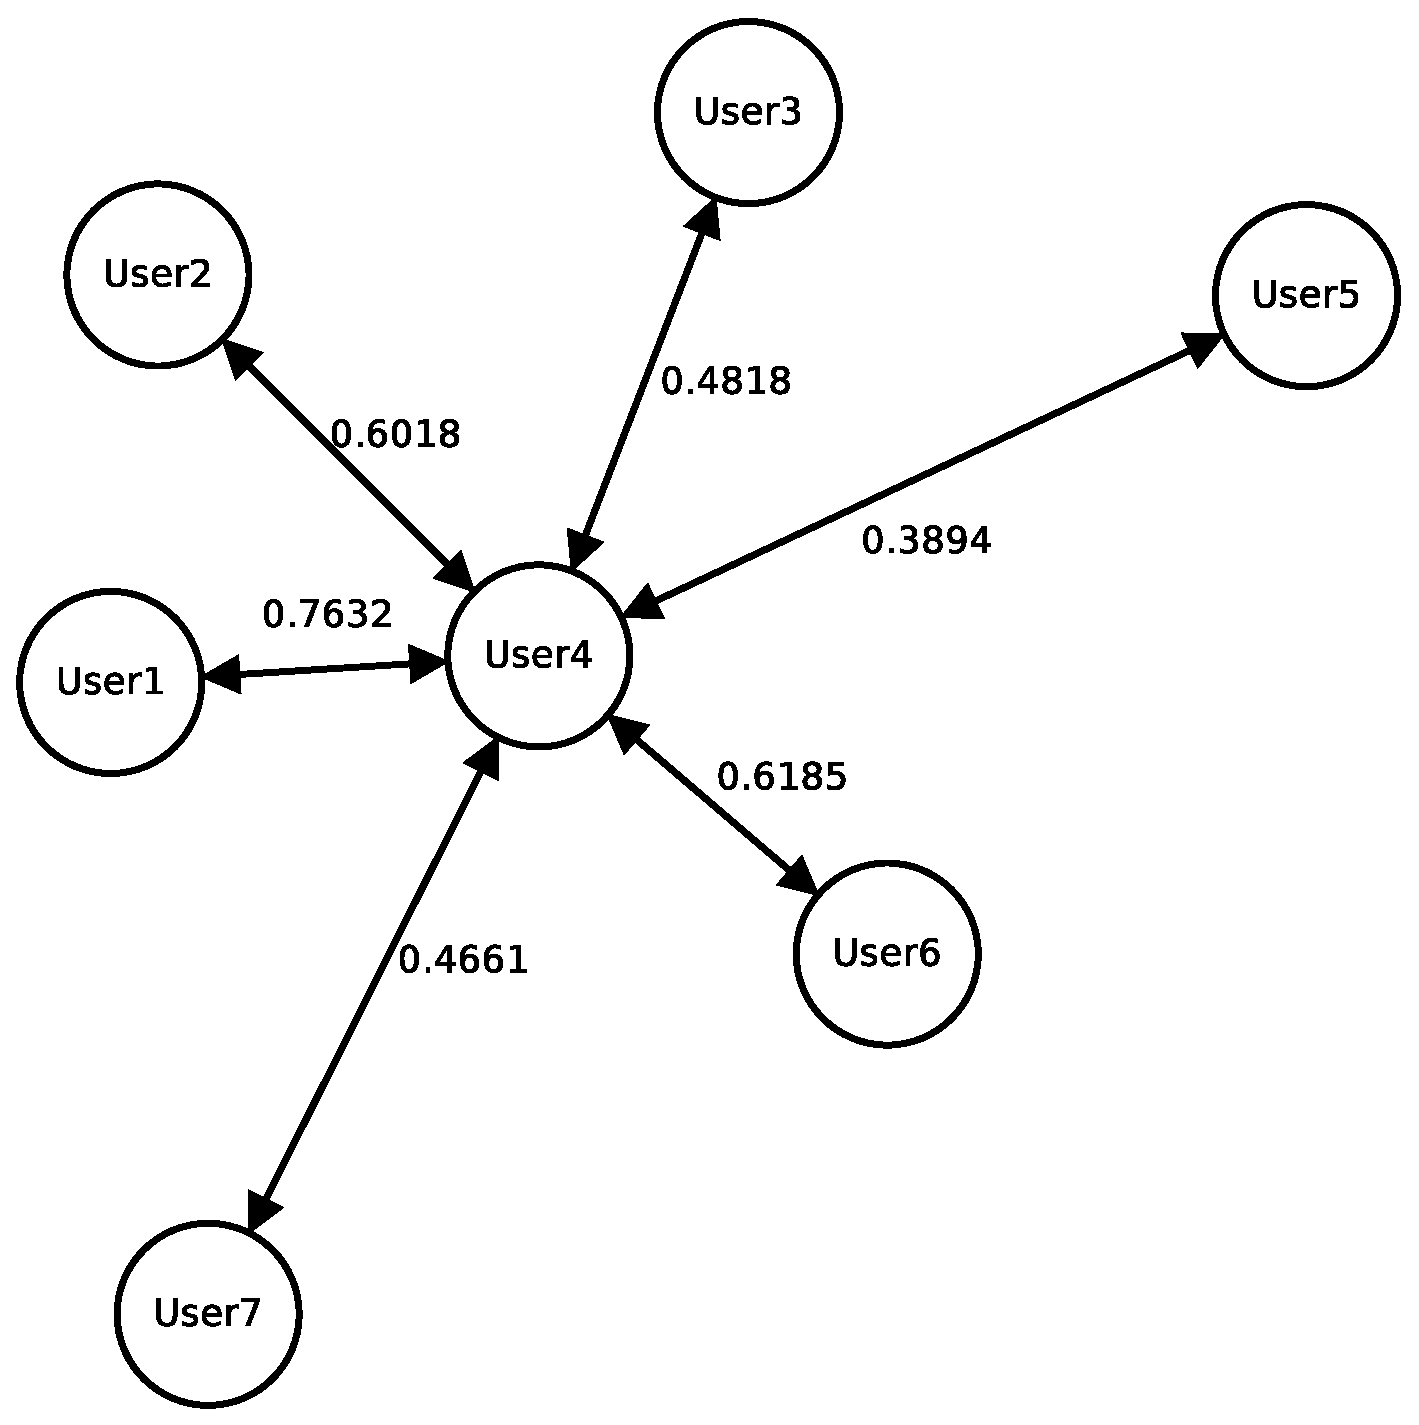
\includegraphics[width=0.5\textwidth]{chapter_2/KNN_example.eps}
	\caption{Cosine Similarities for $User_4$}
	\label{figure:KNN_example}
	\end{figure}
	\item[] \textbf{Step 3:}  Sort that similarities in descending order.
	\begin{align*}
		\begin{split}
			&cos(User_1, User_4) = 0.7632\\
			&cos(User_4, User_6) = 0.6185\\
			&cos(User_2, User_4) = 0.6018\\
			&cos(User_3, User_4) = 0.4818\\
			&cos(User_4, User_7) = 0.4661\\
			&cos(User_4, User_5) = 0.3894\\
		\end{split}
	\end{align*}
	\item[] \textbf{Step 4:}  Choose how many neighbors will contribute in the rating
	prediction in this case we choose for example, $\mathcal{K}=3$.
	\begin{align*}
		\begin{split}
			&cos(User_1, User_4) = 0.7632\\
			&cos(User_4, User_6) = 0.6185\\
			&cos(User_2, User_4) = 0.6018\\
		\end{split}
	\end{align*}
	\begin{figure}[H]
	\centering
	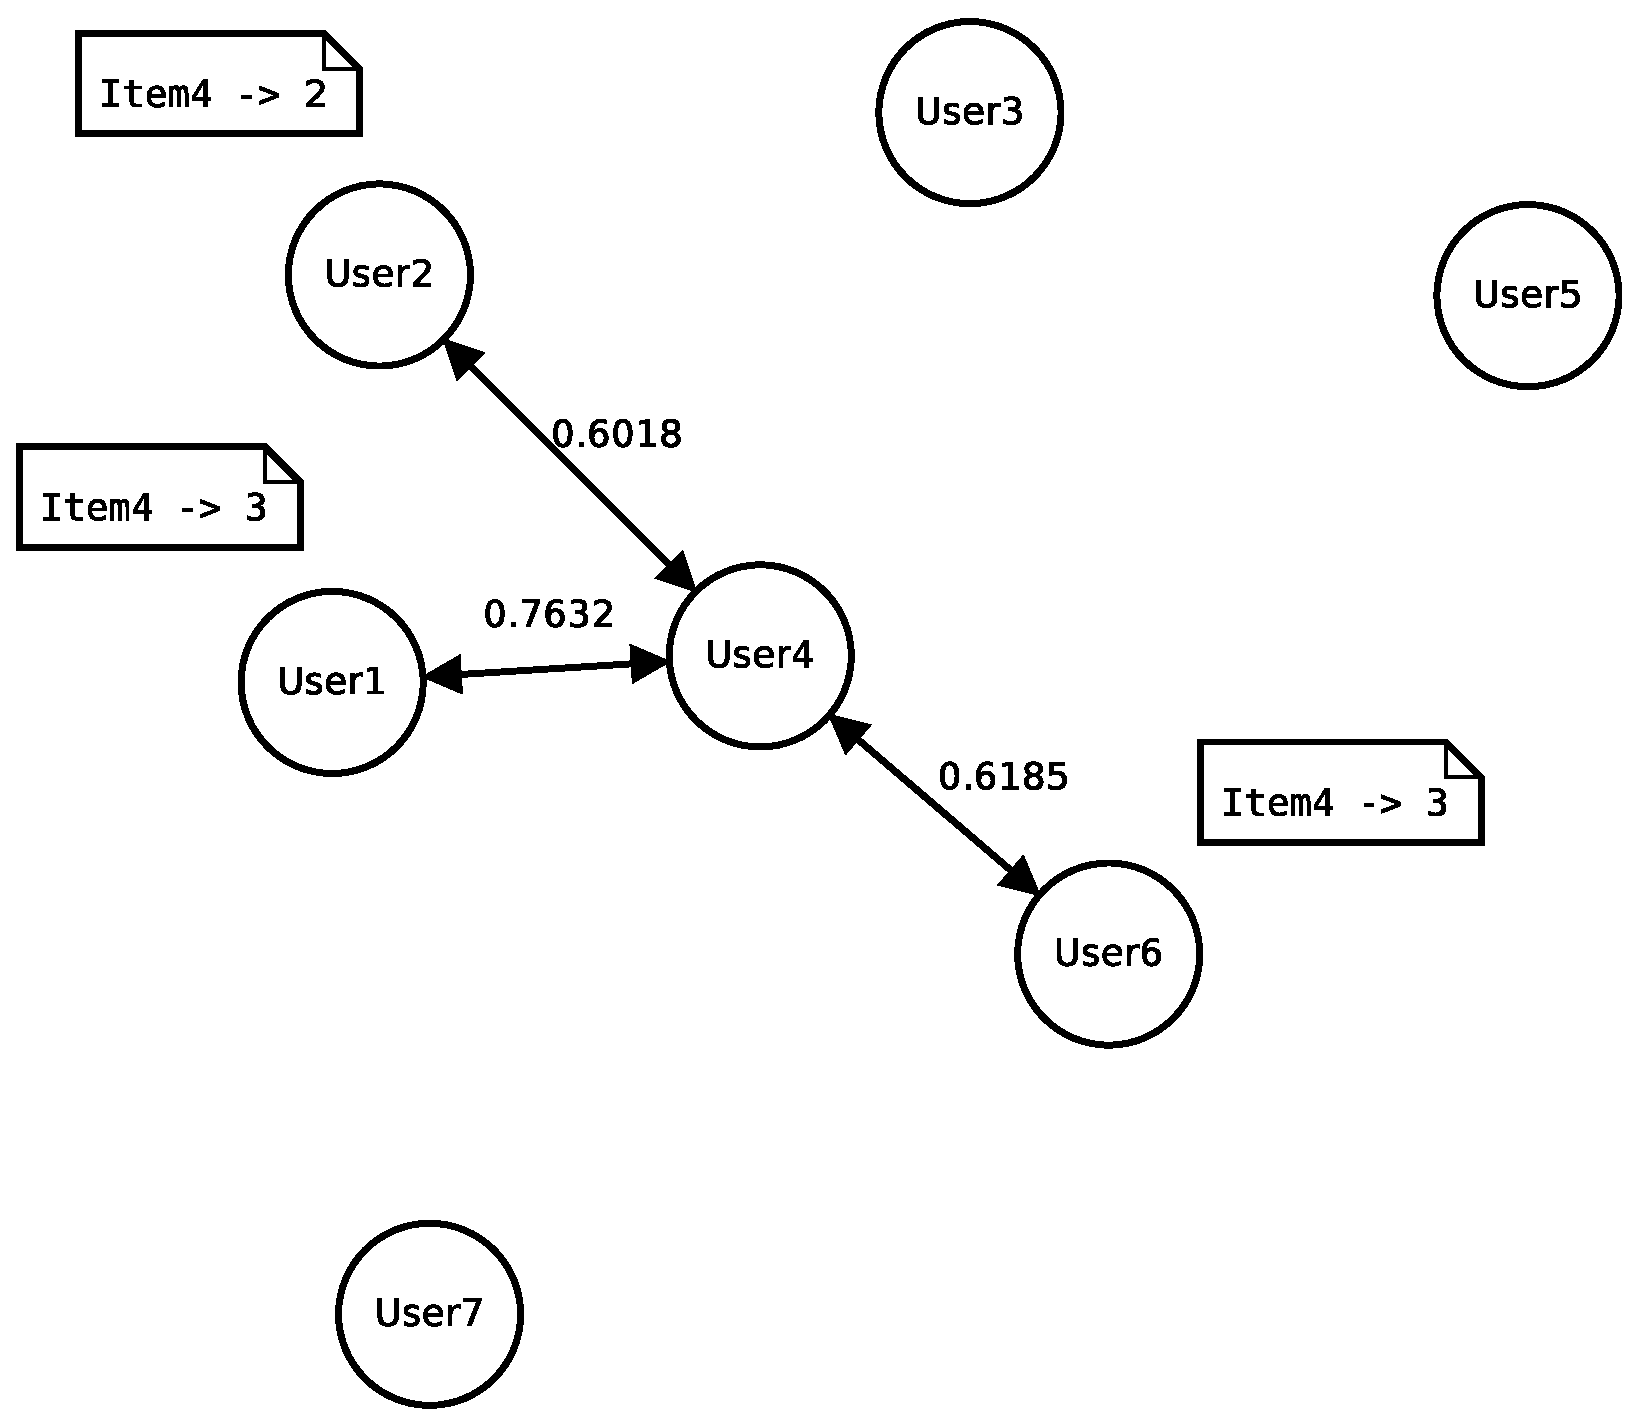
\includegraphics[width=0.5\textwidth]{chapter_2/KNN_example1.eps}
	\caption{Select top $\mathcal{K}=3$ similar users}
	\label{figure:neighbor_selection}
	\end{figure}
	\item[] \textbf{Step 5:} Predict how $User_4$ will rate $Item_4$ using the weighted sum.
	$$\hat{r}(User_4,Item_4) = \frac{0.7632*3 + 0.6018*2 + 0.6185*3}{0.7632 + 0.6018 + 0.6185} = 2.7$$
\end{itemize}


\chapter{Recursive K-Nearest Neighbors}
\label{chap:3}
% !TeX root = ../main.tex

\section{Introduction}
The idea of the recursive nearest neighbors method came up in the process of studying
recommender systems in the framework of this thesis. The method that will be presented is an
effort to overcome the limitations of neighborhood-based approach. That is, to provide more
rating predictions than the conventional K-Nearest Neighbors method, which fails when it
cannot connect users or items directly due to sparseness constraints.

\begin{table}[H]
\centering
\begin{tabular}{ |c|c|c|c|c|c|c| }
\hline
\diagbox{$User$}{$Item$} & \textbf{$Item_1$} & \textbf{$Item_2$} & \textbf{$Item_3$} & \textbf{$Item_4$}  & \textbf{$Item_5$} & \textbf{$Item_6$} \\
\hline
\textbf{$User_1$} & 5 & 2 & 3 & \textbf{?} & 1 & 5 \\
\hline
\textbf{$User_2$} & 1 & 2 & 4 & \textbf{?} & 2 & 2 \\
\hline
\textbf{$User_3$} & 4  & 3 & 5 & \textbf{?} & 4 & 3 \\
\hline
\textbf{$User_4$} & 5 & 2 & 3 &  \textbf{?} & \textbf{?} & \textbf{?} \\
\hline
\textbf{$User_5$} & \textbf{?} & \textbf{?}  & \textbf{?} & 4 & 1 & 1 \\
\hline
\textbf{$User_6$} & \textbf{?} & \textbf{?} & \textbf{?}  & 3 & 5 & 2 \\
\hline
\textbf{$User_7$} & \textbf{?} & \textbf{?} & \textbf{?}  & 5 & 1 & 2 \\
\hline
\textbf{$User_8$} & \textbf{?} & \textbf{?} & \textbf{?}  & 5 & 4 & 4 \\
\hline
\end{tabular}
\caption{Modified Ratings Matrix}
\label{table:Modified Ratings Matrix}
\end{table}

The above table is a modification/extension of \autoref{table:Ratings Matrix}. If KNN was applied to
this rating matrix with $\mathcal{K}=4$(all users do not have 4 available NN, instead
they use the largest amount of NN available to them before 4) using user cosine similarity,
it would produce the rating predictions in the table below.

\begin{table}[H]
\centering
\begin{tabular}{ |c|c|c|c|c|c|c| }
\hline
\diagbox{$User$}{$Item$} & \textbf{$Item_1$} & \textbf{$Item_2$} & \textbf{$Item_3$} & \textbf{$Item_4$}  & \textbf{$Item_5$} & \textbf{$Item_6$} \\
\hline
\textbf{$User_1$} & 5 & 2 & 3 & {\color{red}4.3} & 1 & 5 \\
\hline
\textbf{$User_2$} & 1 & 2 & 4 & {\color{red}4.15} & 2 & 2 \\
\hline
\textbf{$User_3$} & 4  & 3 & 5 & {\color{red}4.12} & 4 & 3 \\
\hline
\textbf{$User_4$} & 5 & 2 & 3 &  {\color{green}\textbf{?}} & {\color{red}2.35} & {\color{red}3.42} \\
\hline
\textbf{$User_5$} & {\color{red}3.35} & {\color{red}2.35}  & {\color{red}4.02} & 4 & 1 & 1 \\
\hline
\textbf{$User_6$} & {\color{red}3.21} & {\color{red}2.4} & {\color{red}4.15}  & 3 & 5 & 2 \\
\hline
\textbf{$User_7$} & {\color{red}3.46} & {\color{red}2.32} & {\color{red}3.94}  & 5 & 1 & 2 \\
\hline
\textbf{$User_8$} & {\color{red}3.36} & {\color{red}2.35} & {\color{red}4.03}  & 5 & 4 & 4 \\
\hline
\end{tabular}
\caption{Modified Ratings Matrix After KNN}
\label{table:Modified Ratings Matrix after KNN}
\end{table}
\justify
It seems that KNN was unable to predict how $User_4$ would rate $Item_4$.\\
The connections from user cosine similarity that could be formed were the following:
\begin{align*}
	&cos(User_1,User_2) = 0.7659 &cos(User_1,User_3) = 0.8660 & &cos(User_1,User_4) = 0.7705\\
	&cos(User_1,User_5) = 0.1767 &cos(User_1,User_6) = 0.3041 & &cos(User_1,User_7) = 0.2510\\
	&cos(User_1,User_8) = 0.3973 &cos(User_2,User_3) = 0.9434 & &cos(User_2,User_4) = 0.6325\\
	&cos(User_2,User_5) = 0.1750 &cos(User_2,User_6) = 0.4217 & &cos(User_2,User_7) = 0.2034\\
	&cos(User_2,User_8) = 0.3935 &cos(User_3,User_4) = 0.7680 & &cos(User_3,User_5) = 0.1905\\
	&cos(User_3,User_6) = 0.4870 &cos(User_3,User_7) = 0.2108 & &cos(User_3,User_8) = 0.4282\\
	&cos(User_5,User_6) = 0.7264 &cos(User_5,User_7) = 0.9897 & &cos(User_5,User_8) = 0.8741\\
	&cos(User_6,User_7) = 0.7108 &cos(User_6,User_8) = 0.9239 & &cos(User_7,User_8) = 0.8947\\
\end{align*}
\vfill
\justify
The following figure is a graphical representation of the user connections.
\begin{figure}[H]
\centering
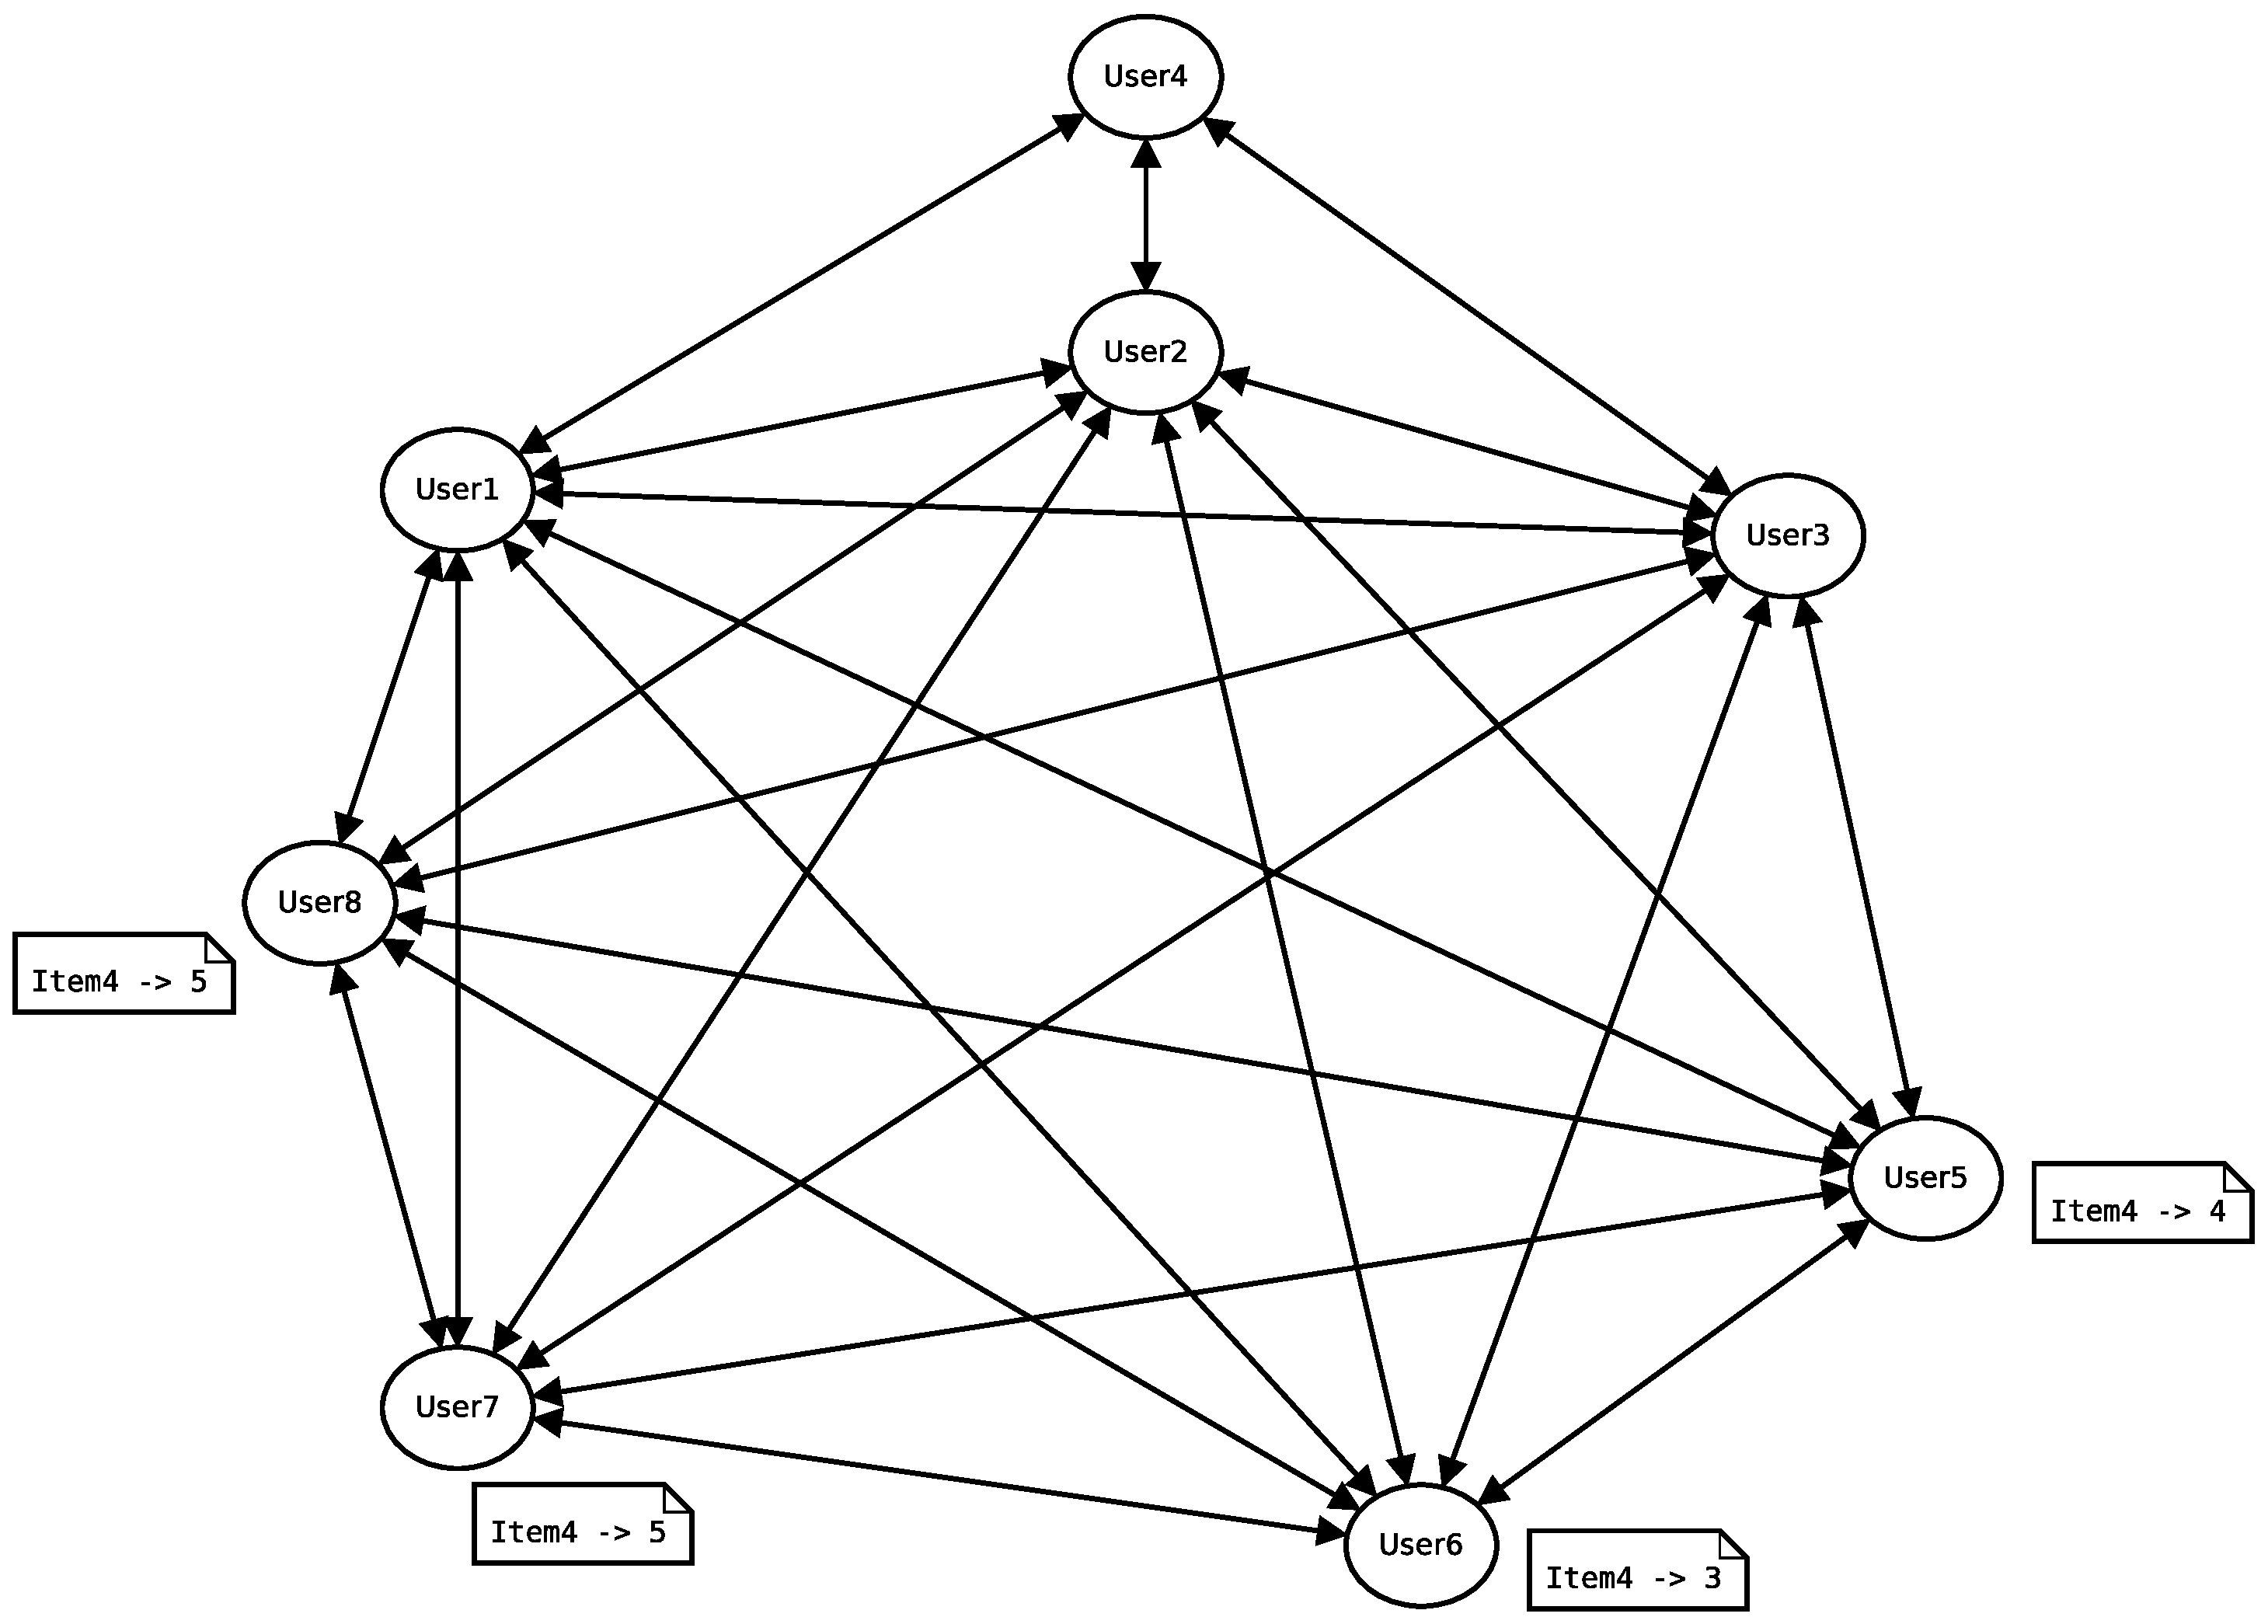
\includegraphics[width=0.8\textwidth]{chapter_3/user_connections.eps}
\caption{User Connections}
\label{figure:user_connections}
\end{figure}

It seems that from users who have rated $Item_4$, it is possible to create a connection to $User_4$, but in
order to do that they must use the intermediate connections they have in common. Graph-based
methods are known to utilize these connections efficiently to produce link similarities that
surpass the direct connection between users or items \citep{Ricci,Aggarwal}.
\section{Methodology}
The Recursive K-Nearest Neighbors algorithm utilizes the intermediate connections that two users
have in common in order to find a path to predict ratings that the conventional KNN could not find.
The concept of this algorithm, is to use the rating predictions produced by KNN, in order
to consider the users that have not rated the target item, as neighbors. As presented in
\autoref{figure:user_connections_with_KNN} below,
the KNN rating predictions related to $Item_4$ for $User_1$, $User_2$ and $User_3$ have been
added to the figure to indicate them as real rating values that these users gave to $Item_4$.
\begin{figure}[H]
\centering
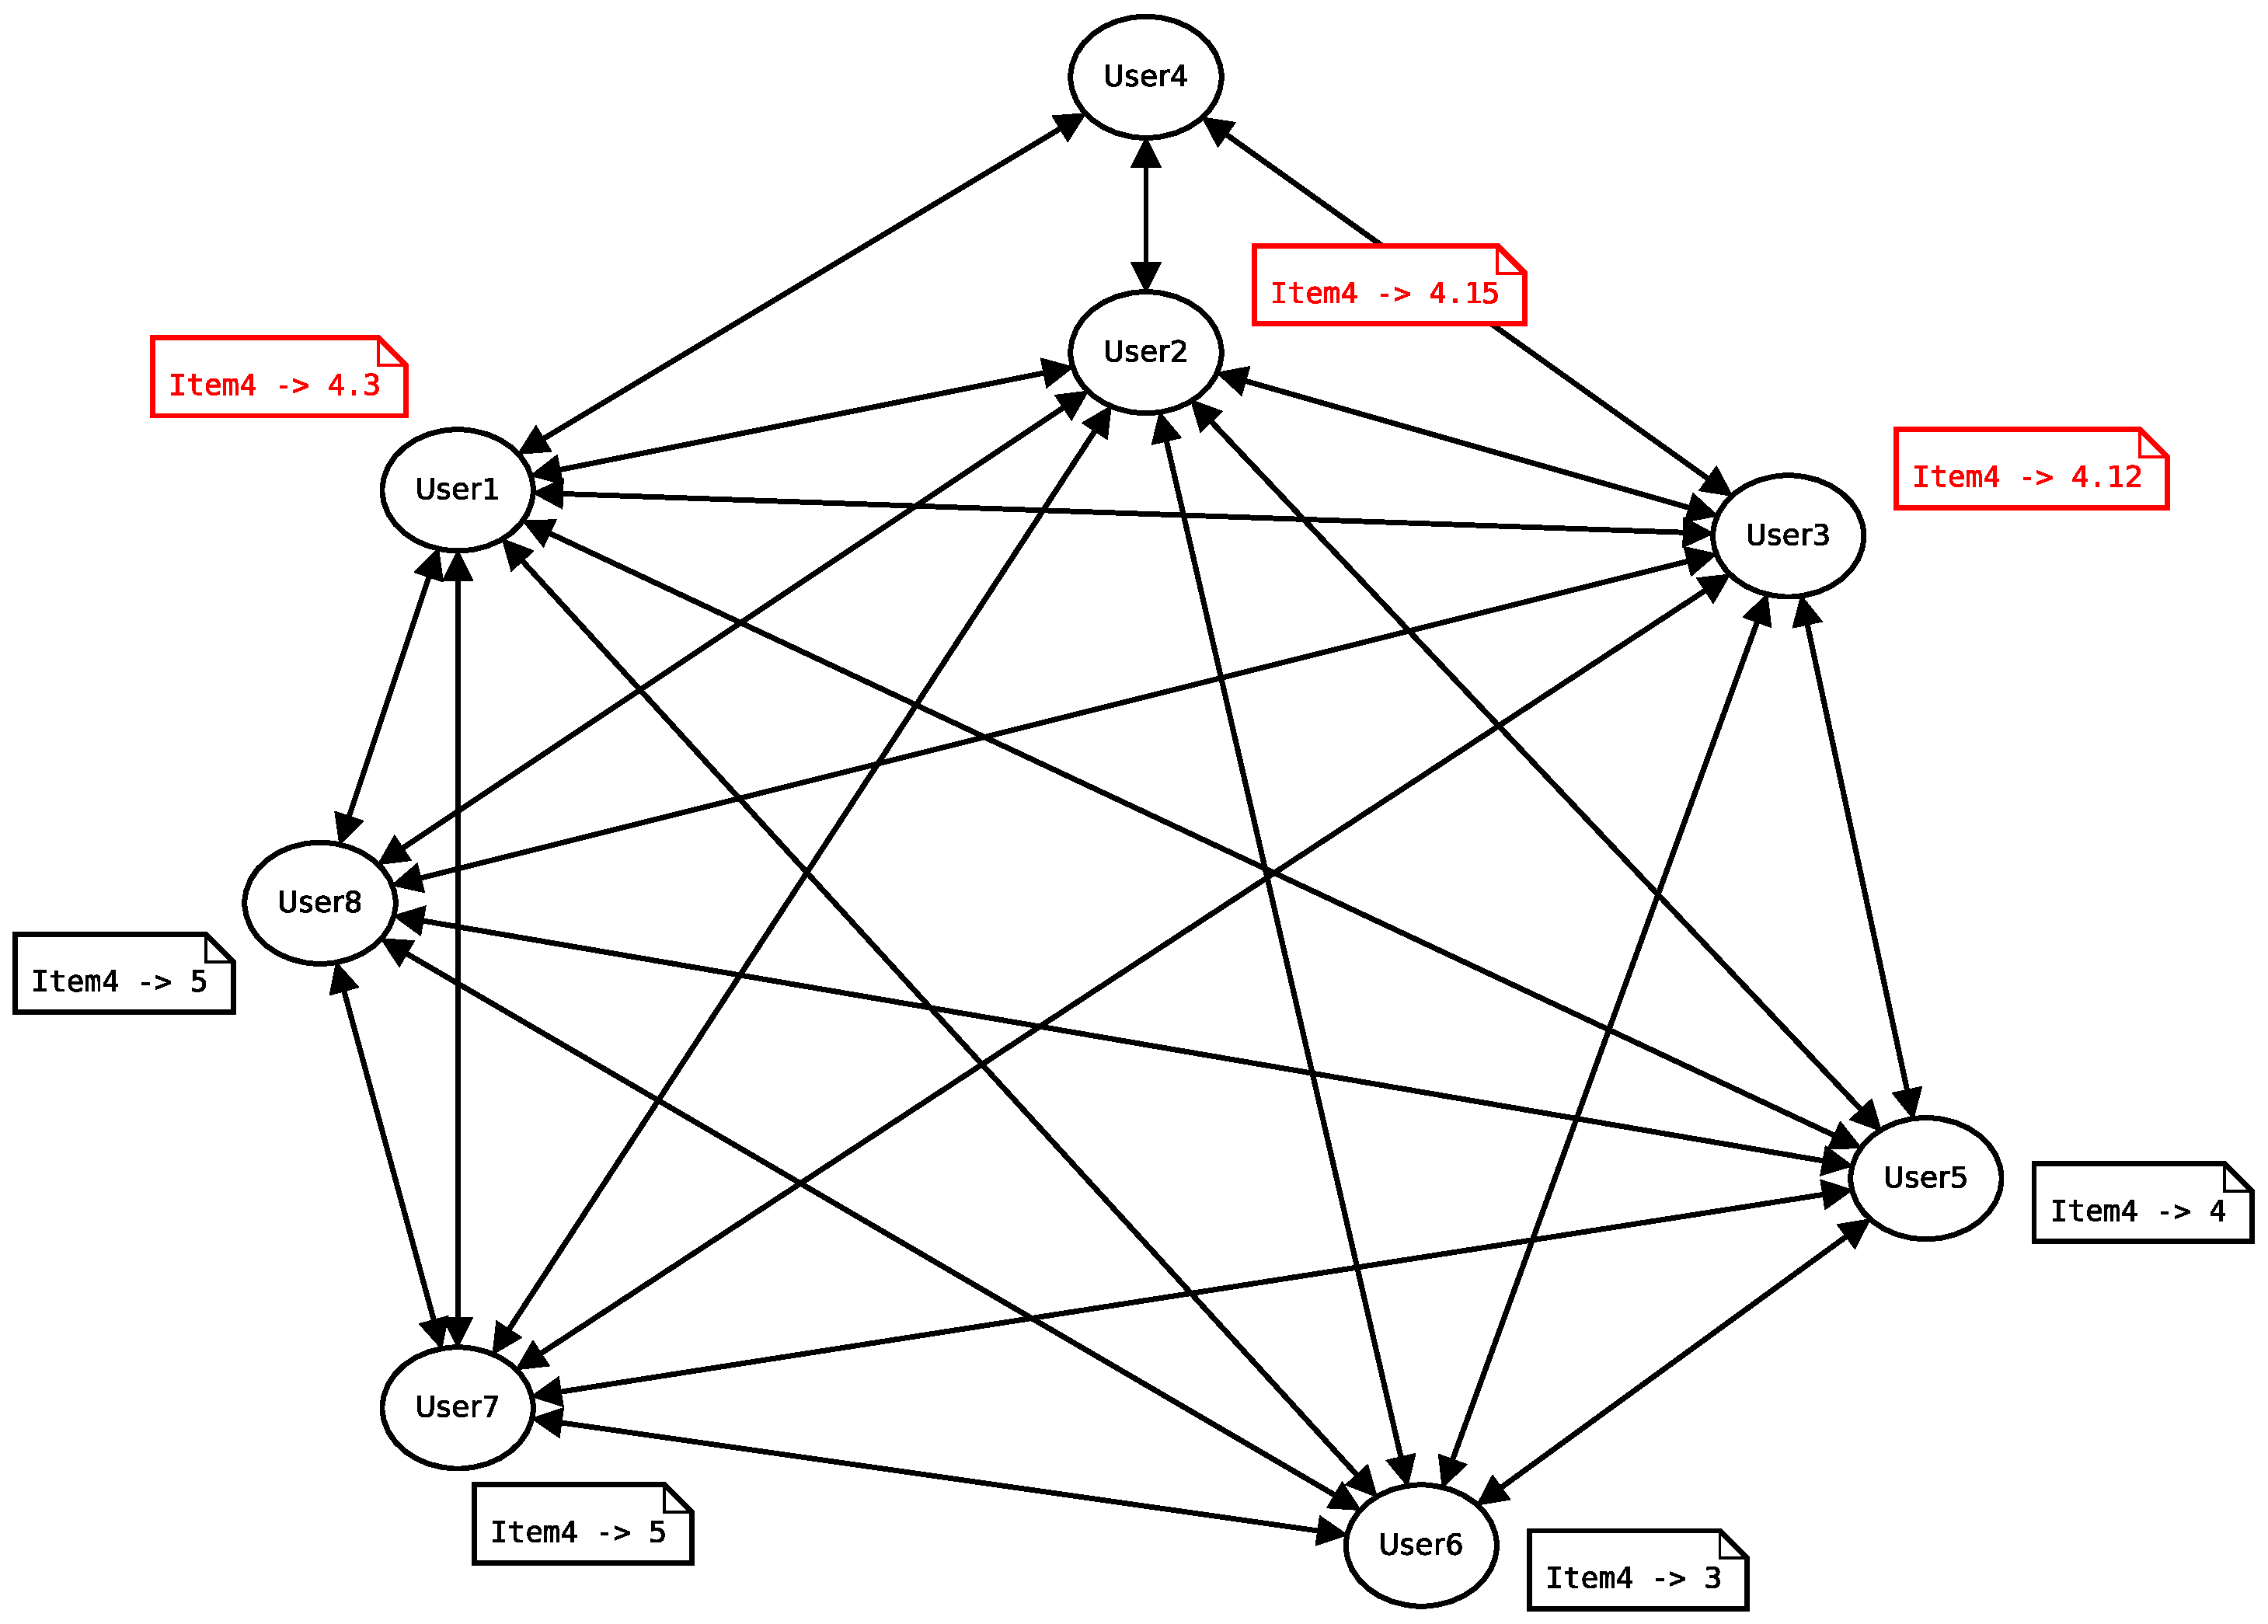
\includegraphics[width=0.8\textwidth]{chapter_3/user_connections_with_KNN.eps}
\caption{User Connections as \autoref{figure:user_connections} with KNN predictions from \autoref{table:Modified Ratings Matrix after KNN}}
\label{figure:user_connections_with_KNN}
\end{figure}
Then, as new similarities can be formed for $User_4$ with $User_1$, $User_2$ and $User_3$ for $Item_4$, the weighted sum formula used in KNN can be
again used to compute the rating prediction of $User_4$ to $Item_4$ as shown in \autoref{figure:RKNN_prediction}.\\
\begin{figure}[H]
\centering
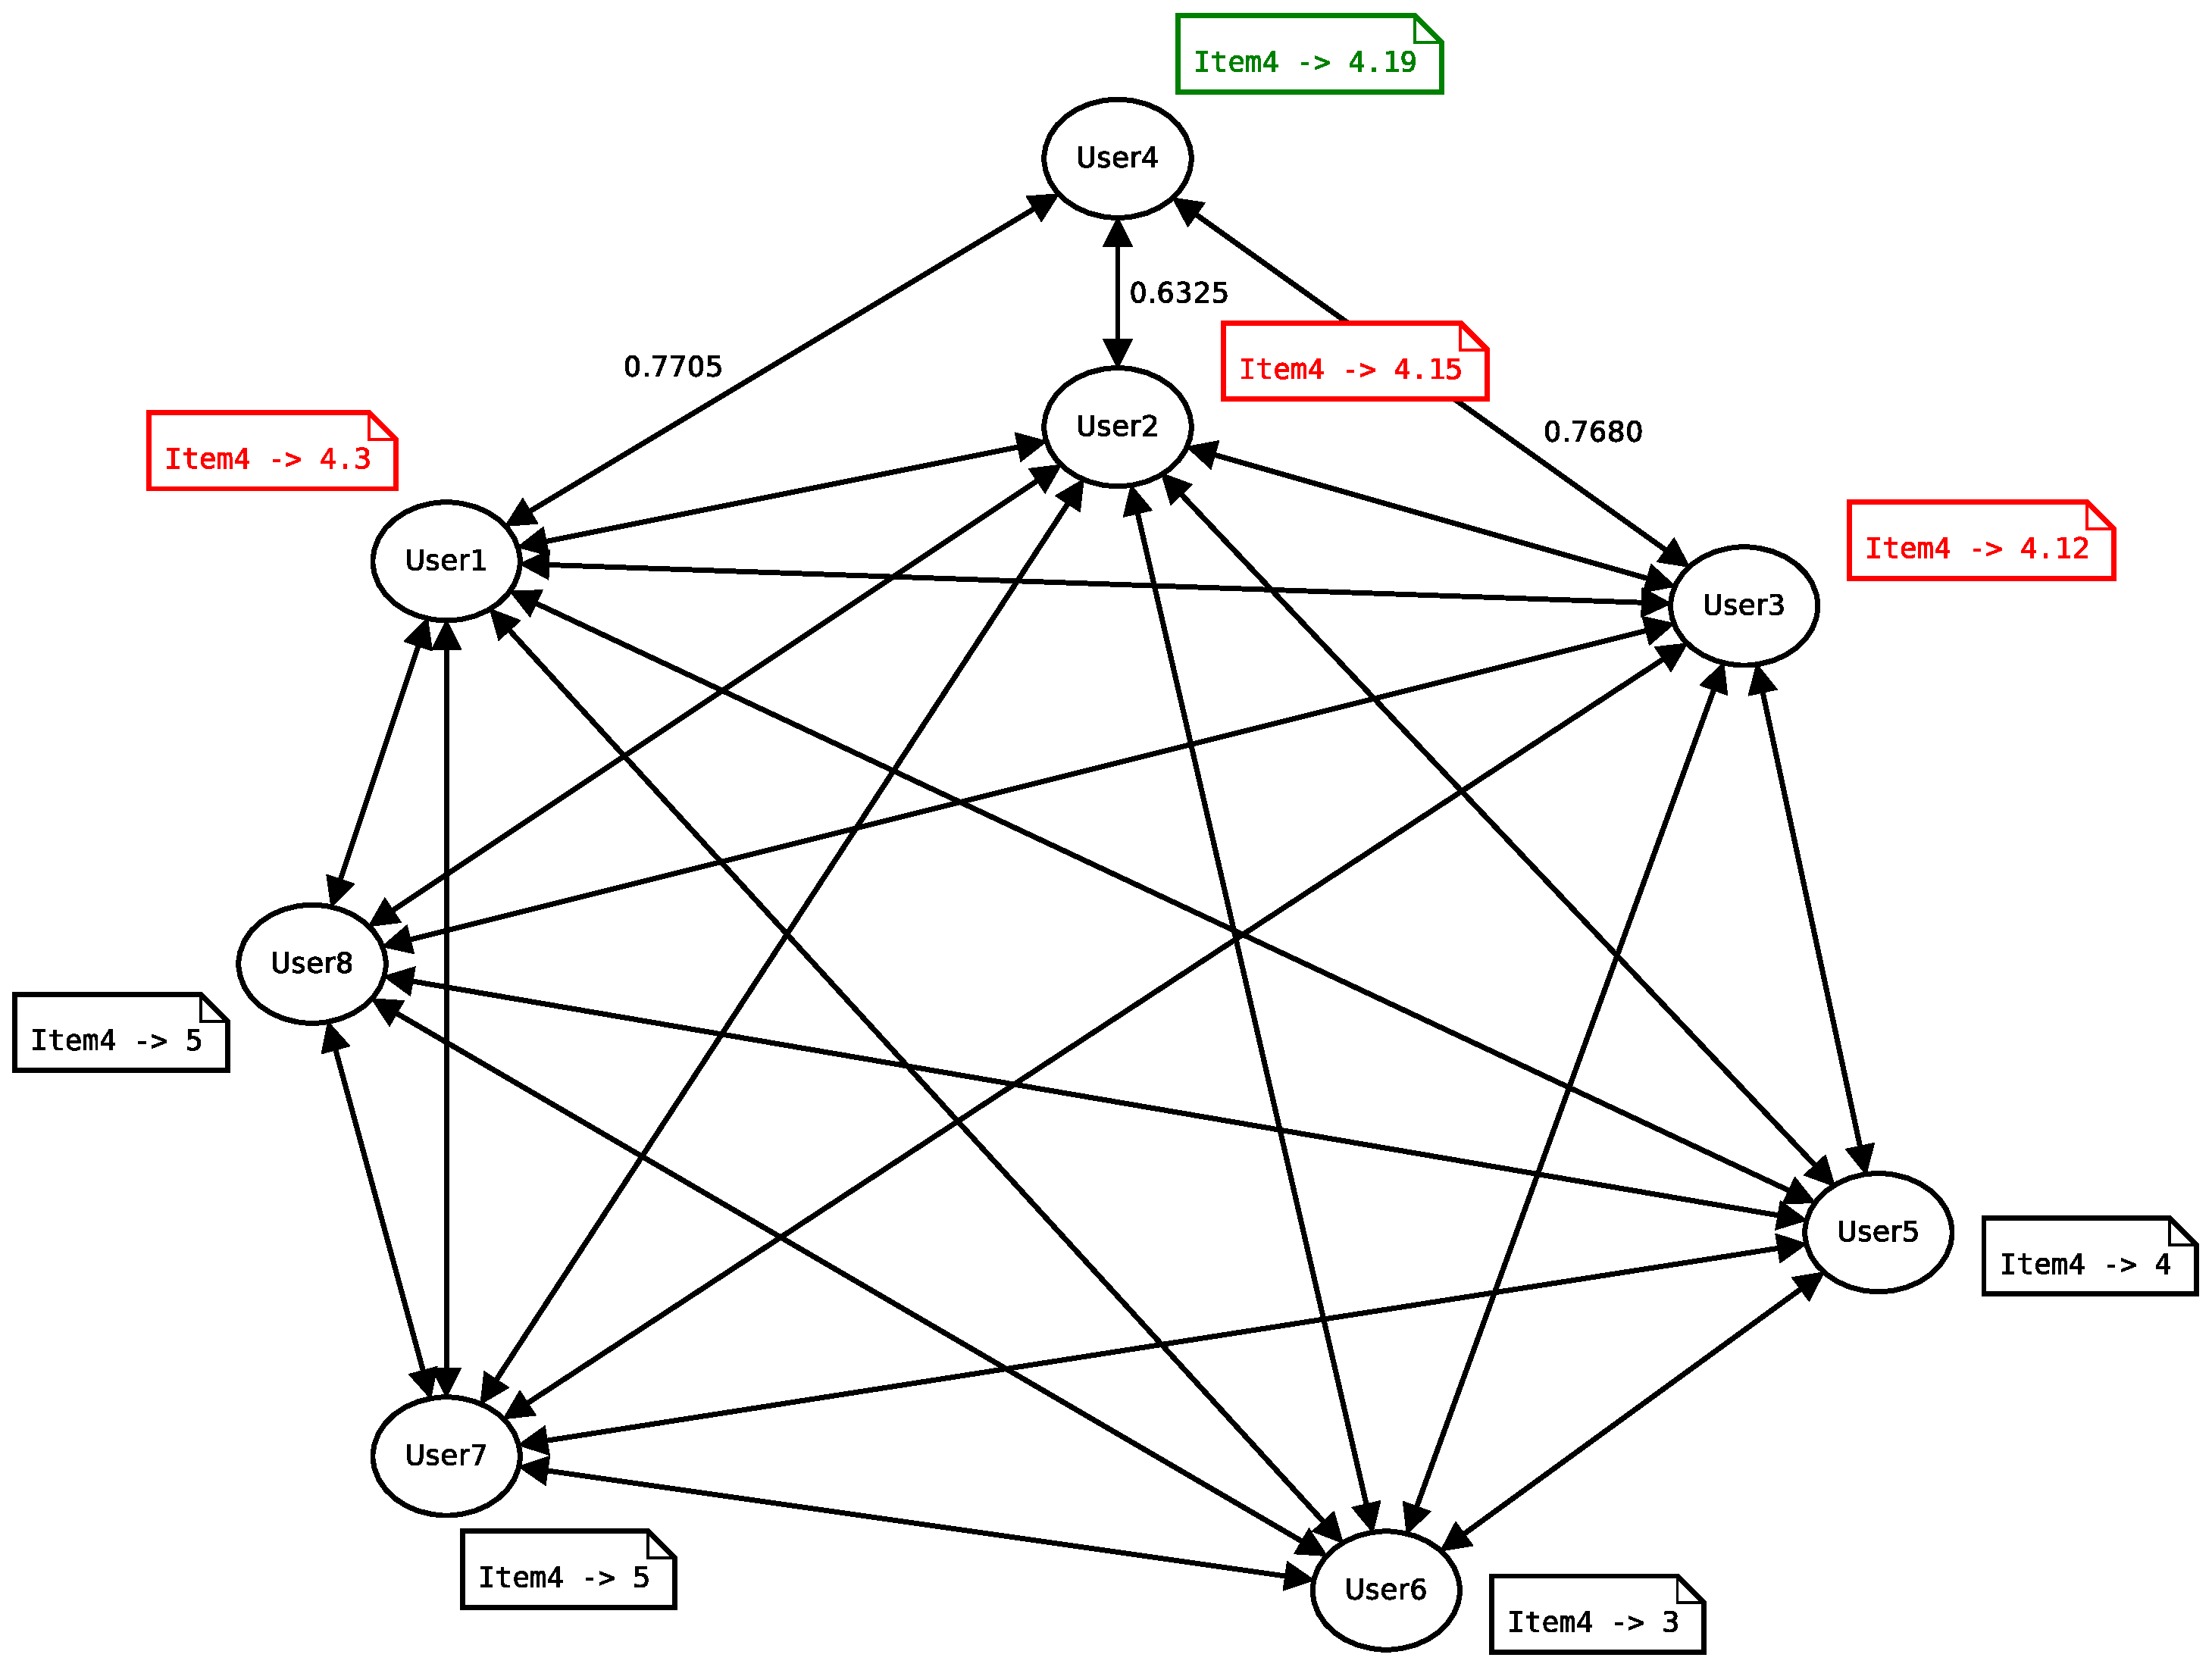
\includegraphics[width=0.8\textwidth]{chapter_3/RKNN_prediction.eps}
\caption{Recursive KNN Rating Prediction}
\label{figure:RKNN_prediction}
\end{figure}
The Recursive K-Nearest Neighbors methodology for predicting how $User_A$ would rate $Item_B$,
(with the assumption that, given a similarity metric, KNN would not be able to predict this rating)
consists of the following steps:
\begin{itemize}\label{RKNN}
	\item[] \textbf{Step 1:} Select users that are connected with $User_A$, and name it $Group_A$.
	\item[] \textbf{Step 2:} Out of $Group_A$, choose those users that have connections with
	users who have rated $Item_B$, and name it $Group_B$.
	\item[] \textbf{Step 3:}  Order $Group_B$ by descending similarity with $User_A$.
	\item[] \textbf{Step 4:}  Choose how many neighbors from $Group_B$ will contribute in the
	rating prediction by selecting the top $\mathcal{K}$ out of all the available
	neighbors in this group, and name it $Group_C$.
	\item[] \textbf{Step 5:} For each neighbor in $Group_C$, predict how this neighbor would
	rate $Item_B$ using the KNN algorithm. For convenience, we name the number of recursive
	neighbors each neighbor in $Group_C$ uses as, $\mathcal{M}$-Nearest Neighbors.
	\item[] \textbf{Step 6:} Use the rating predictions applied on $Group_C$ to perform
	the KNN algorithm on $User_A$ for $Item_B$.
\end{itemize}

Now that the steps for performing the Recursive K-Nearest Neighbors algorithm have been
introduced let us look at a general case as in the figure below:\\
\begin{figure}[H]
\centering
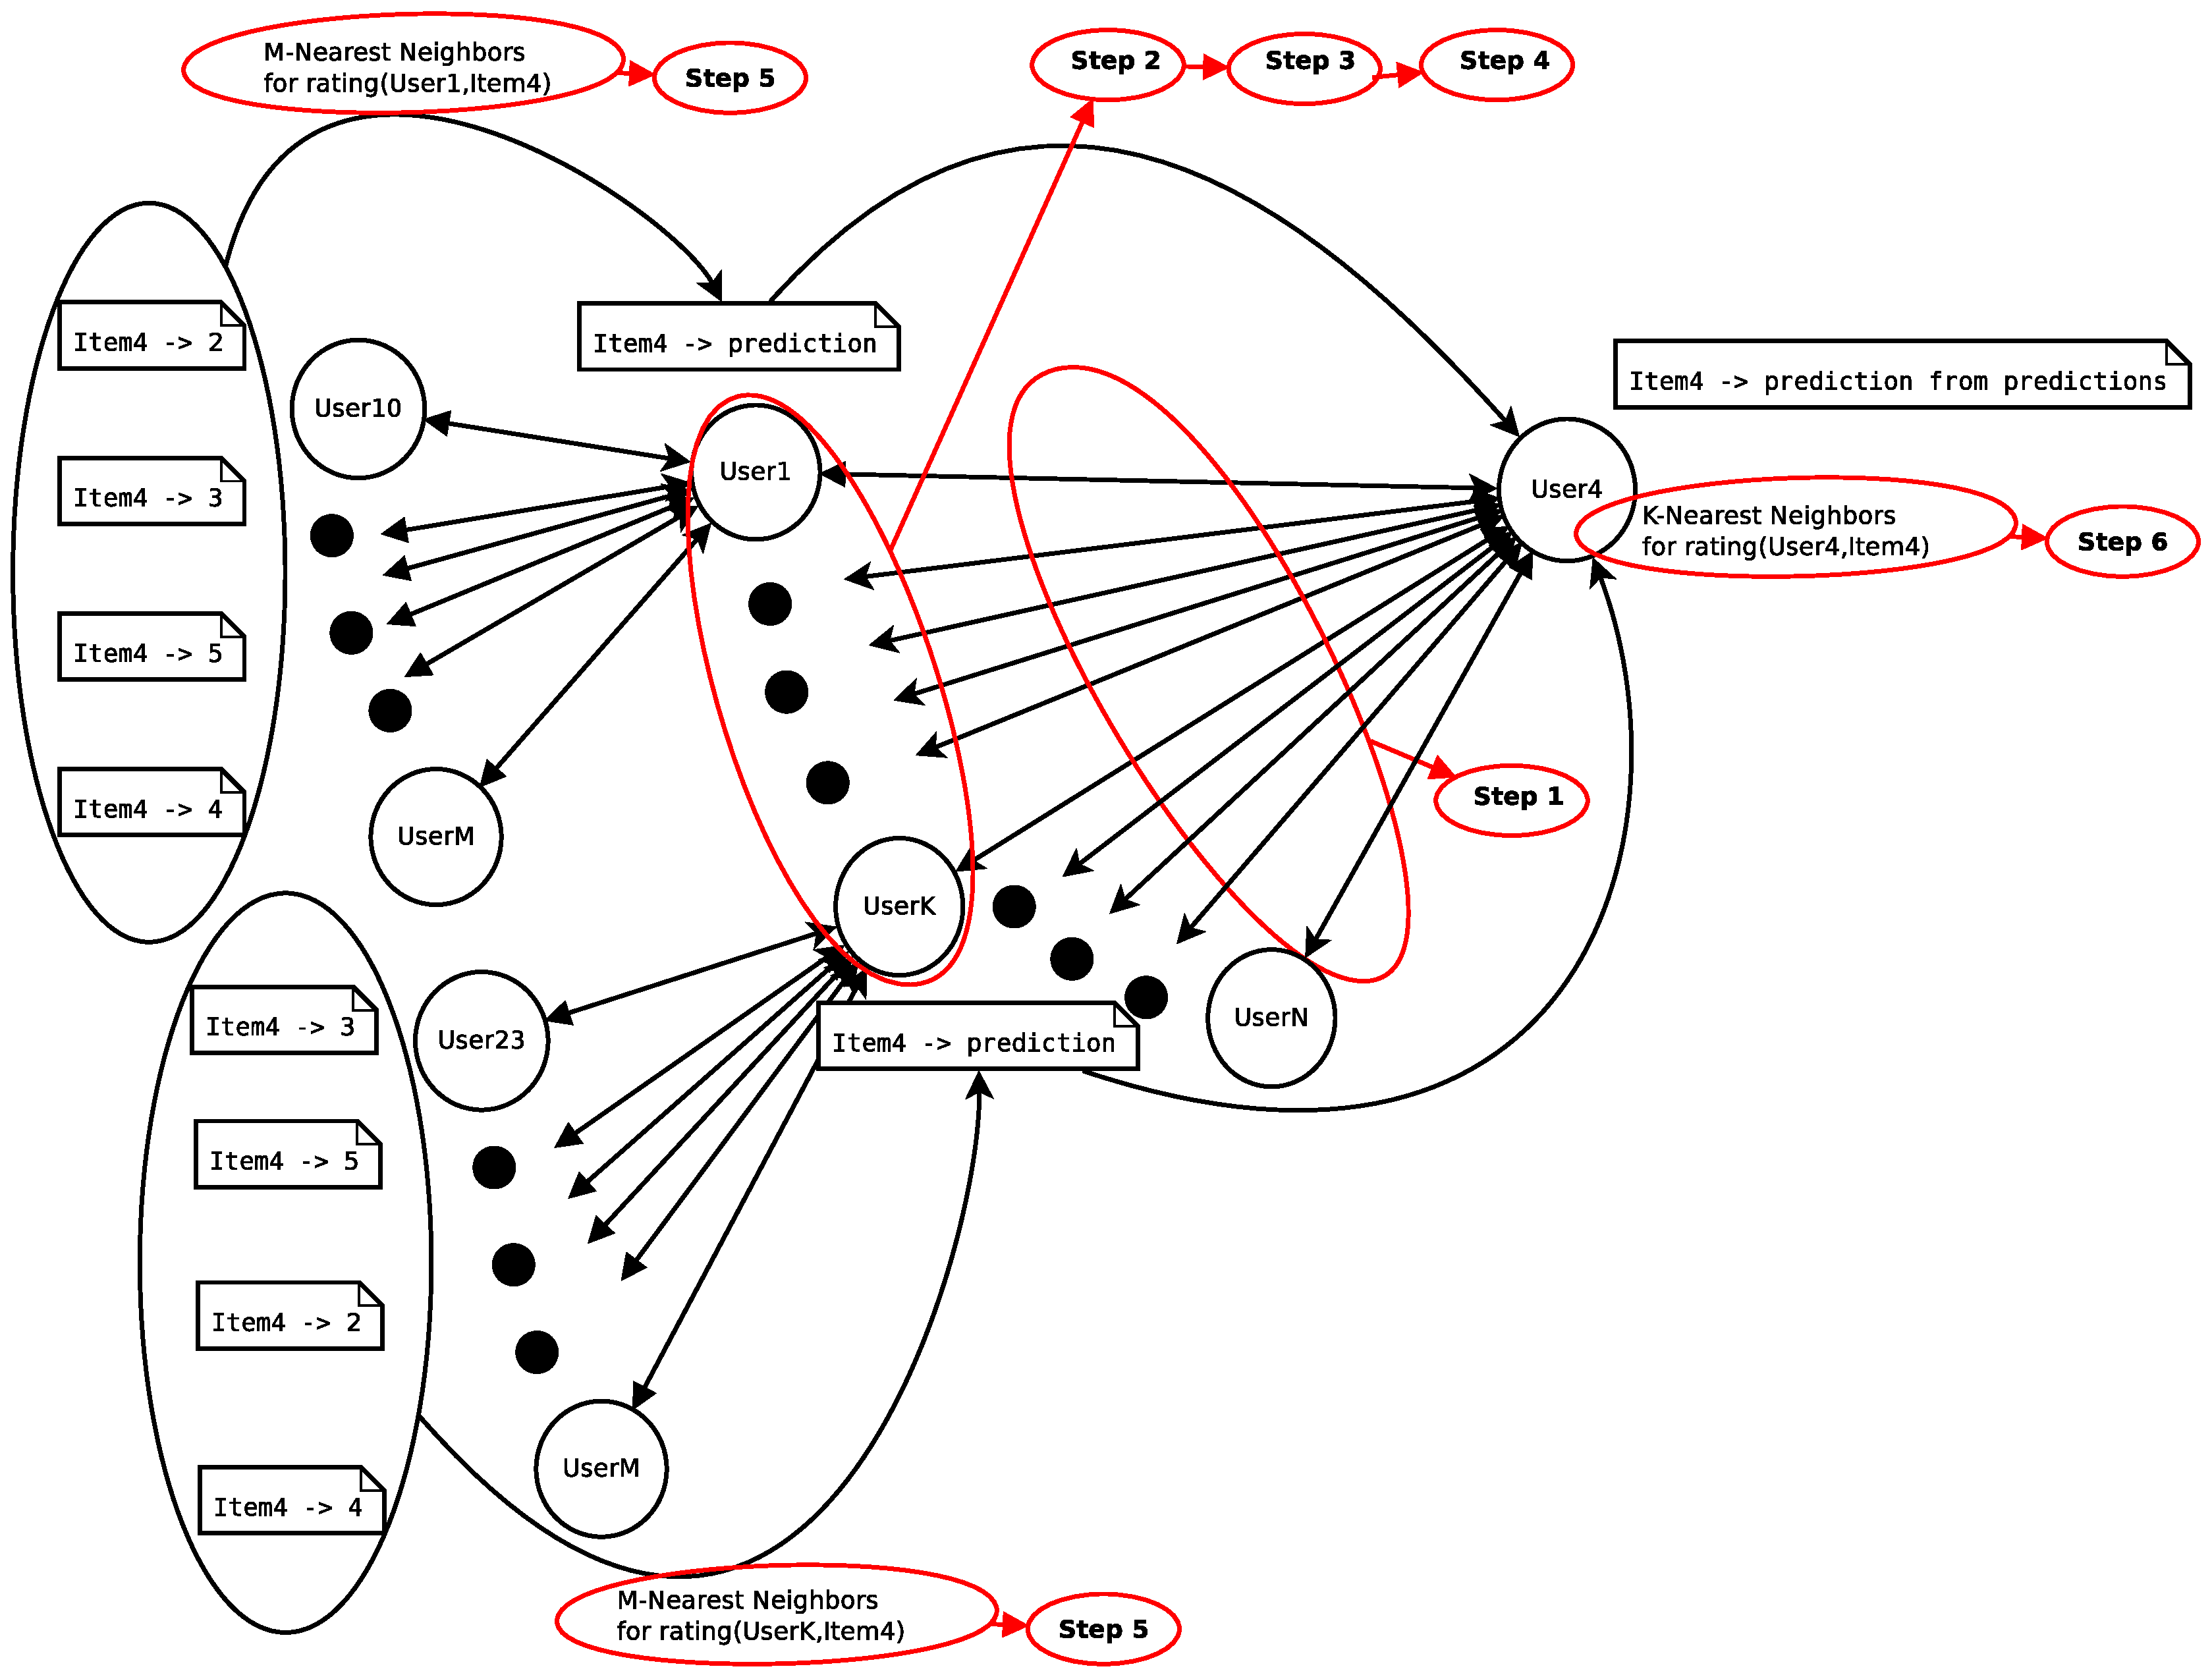
\includegraphics[width=0.8\textwidth]{chapter_3/Recursive_Nearest_Neighbors.eps}
\caption{Recursive Nearest Neighbors Algorithm}
\label{figure:recursive_algorithm}
\end{figure}
Interpretation of the figure:
\begin{enumerate}
	\item After the selection of the top $\mathcal{K}$ relevant Neighbors.
	(\textbf{Steps 1,2,3,4})
	\item For each Neighbor, name it $Neighbor_i$, out of $\mathcal{K}$'s choose $\mathcal{M}$
	Neighbors to apply KNN on $Neighbor_i$. (\textbf{Step 5})
	\item Use the rating predictions applied on $\mathcal{K}$'s to predict the requested
	User-Item rating.\\ (\textbf{Step 6})
\end{enumerate}


\chapter{Evaluation}
\label{chap:4}
% !TeX root = ../main.tex

\section{Data set}
The Epinions data set \citep{Massa} is a very good case to demonstrate the Recursive
K-Nearest Neighbors algorithm because of its sparsity. As demonstrated in \autoref{chap:3},
this algorithm manages to overcome the limitations of the conventional KNN algorithm, which
cannot make predictions for ratings with no direct associations to other users or items.
This dataset consists of 40163 users and 139738 items and 664824 ratings.
As we mentioned previously, the sparsity percentage is 0,99988154.
The structure of the dataset is shown in the table below:
\begin{table}[H]
\centering
\caption{Epinions Dataset Sample}
\label{table:Epinions_sample}
\begin{tabular}{ |c|c|c| }
\hline
\textbf{user} & \textbf{item} & \textbf{Rating} \\
\hline
36153 & 62461 & 5 \\
\hline
427 & 38005 & 5  \\
\hline
751 & 53361 & 4 \\
\hline
11001 & 118950 & 4 \\
\hline
1169 & 66176 & 5 \\
\hline
9808 & 84459 & 2 \\
\hline
85 & 7446 & 4 \\
\hline
14717 & 3397 & 2 \\
\hline
\end{tabular}
\end{table}
The user and item columns contain the ids of users and items respectively, and the rating
column contains the rating of a user to an item. To test the accuracy of
KNN and Recursive-KNN algorithms this ratings matrix was split in a
train set and a test set. The train set is used so the algorithms can learn the
patterns of the data. Either how users rate or how items are being rated.
The similarity metrics discussed in \autoref{chap:2} will be computed based on
the train set and the rating predictions will be calculated based on this set's
ratings. The rating predictions will be both user-based and item based.
The test set is used to evaluate the rating predictions produced by the trained algorithms
to this set using an aggregating error function between the predictions
and the truth values. The train set consists of 520203
ratings(78\%) and the test set consists of 144621 ratings(22\%). The train
set is stratified by users, which means that it contains a proportion of each
user's ratings. Below there are some descriptive information about the Epinions dataset and the splitting method.
\begin{table}[H]
\centering
\caption{Epinions Descriptive}
\label{table:epinions_descriptive}
\begin{tabular}{ |c|c|c|c| }
\hline
&\textbf{Ratings Matrix} & \textbf{Train} & \textbf{Test}\\
\hline
count & 664824 & 520203 & 144621\\
\hline
mean & 3.9917 & 3.99 & 3.9975\\
\hline
std & 1.2068 & 1.2072 & 1.2053\\
\hline
min & 1 & 1 & 1\\
\hline
25\% & 3 & 3 & 3\\
\hline
50\% & 4 & 4 & 4\\
\hline
75\% & 5 & 5 & 5\\
\hline
max & 5 & 5 & 5\\
\hline
\end{tabular}
\end{table}

In the subsections below we present some basic descriptive information about each of the similarity
methods and in \autoref{sec:4.3} we will present the best result from the
rating predictions.

\subsection{Cosine Similarity}

\begin{figure}[H]
\centering
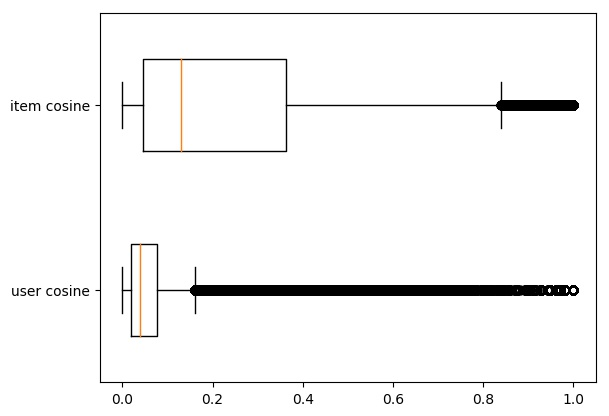
\includegraphics[width=0.7\textwidth]{chapter_4/boxplots/cosine/cosine_boxplot.jpg}
\caption{Cosine Similarity Boxplot (Whiskers= -+1.5IQR)}
\label{figure:cosine_similarity_boxplot}
\end{figure}

Both item and user similarity values have a minimum value near zero.The items' right whisker value is
around 0.8 and the users' around 0.18. Both items and users similarity outliers seem to reach the value of 1.
Also the number of outliers in item cosine appears significantly lower than that of the users.
At least 75\% of users similarities are lower than 0.1. In contrast, at least 50\% of
item similarities are larger than 0.1 and at least 25\% are larger than 0.35.

\begin{table}[H]
\centering
\caption{Cosine Similarity Descriptive}
\label{table:cosine_similarity_descriptive}
\begin{tabular}{|c|c|c|}
\hline
		  & \textbf{users} & \textbf{items} \\ \hline
count     & 14614164       & 18672616       \\ \hline
mean      & 0.063717709    & 0.2590515005   \\ \hline
std       & 0.0852396246   & 0.2948759498   \\ \hline
min       & 0.0001118907   & 0.0001876405   \\ \hline
25\%      & 0.0184512236   & 0.0467473495   \\ \hline
50\%      & 0.0389925088   & 0.1290322581   \\ \hline
75\%      & 0.0758098044   & 0.3638034376   \\ \hline
max       & 1              & 1              \\ \hline
max count & 26742          & 1519527        \\ \hline
min count & 1              & 1              \\ \hline
\end{tabular}
\end{table}

\begin{table}[H]
\centering
\caption{Cosine Similarity Count Descriptive}
\label{table:cosine_similarity_count_descriptive}
\begin{tabular}{|c|c|c|}
\hline
          & \textbf{users}  & \textbf{items} \\ \hline
count     & 39156           & 121140         \\ \hline
mean      & 746.4584737971  & 308.281591547  \\ \hline
std       & 1174.5013754664 & 666.5799806645 \\ \hline
min       & 1               & 1              \\ \hline
25\%      & 40              & 37             \\ \hline
50\%      & 246             & 120            \\ \hline
75\%      & 944             & 338            \\ \hline
max       & 13843           & 31057          \\ \hline
max count & 1               & 1              \\ \hline
min count & 793             & 545            \\ \hline
\end{tabular}
\end{table}

\subsection{Modified Cosine Similarity}

\begin{figure}[H]
\centering
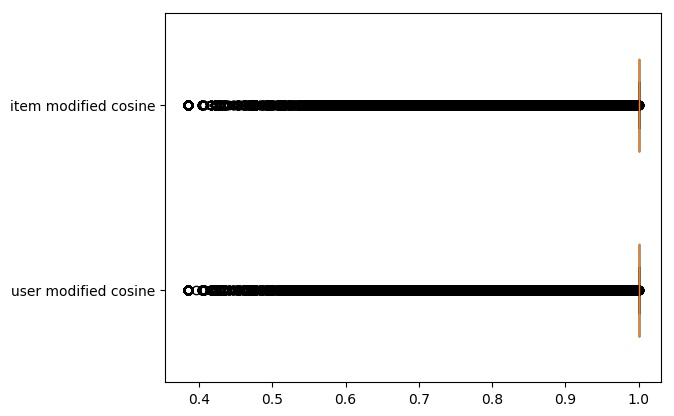
\includegraphics[width=0.9\textwidth]{chapter_4/boxplots/modified_cosine/modified_cosine_boxplot.jpg}
\caption{Modified Cosine Similarity Boxplot (Whiskers= -+1.5IQR)}
\label{figure:modified_cosine_similarity_boxplot}
\end{figure}

Modified cosine similarity seems to have the same effect in the values for both items
and users. Both these boxplots have the majority of their values at 1. Their minimum values
are a little less than 0.4. Any value other than 1 can be interpreted as an outlier.

\begin{table}[H]
\centering
\caption{Modified Cosine Similarity Descriptive}
\label{table:modified_cosine_similarity_descriptive}
\begin{tabular}{|c|c|c|}
\hline
          & \textbf{users} & \textbf{items} \\ \hline
count     & 14614164       & 18672616       \\ \hline
mean      & 0.9923727737   & 0.9970178776   \\ \hline
std       & 0.0345699768   & 0.0205710501   \\ \hline
min       & 0.3846153846   & 0.3846153846   \\ \hline
25\%      & 1              & 1              \\ \hline
50\%      & 1              & 1              \\ \hline
75\%      & 1              & 1              \\ \hline
max       & 1              & 1              \\ \hline
max count & 12887451       & 17728374       \\ \hline
min count & 1170           & 263            \\ \hline
\end{tabular}
\end{table}

\begin{table}[H]
\centering
\caption{Modified Cosine Similarity Count Descriptive}
\label{table:modified_cosine_similarity_count_descriptive}
\begin{tabular}{|c|c|c|}
\hline
          & \textbf{users}  & \textbf{items} \\ \hline
count     & 39156           & 121140         \\ \hline
mean      & 746.4584737971  & 308.281591547  \\ \hline
std       & 1174.5013754664 & 666.5799806645 \\ \hline
min       & 1               & 1              \\ \hline
25\%      & 40              & 37             \\ \hline
50\%      & 246             & 120            \\ \hline
75\%      & 944             & 338            \\ \hline
max       & 13843           & 31057          \\ \hline
max count & 1               & 1              \\ \hline
min count & 793             & 545            \\ \hline
\end{tabular}
\end{table}

\subsection{Adjusted Cosine Similarity}

\begin{figure}[H]
\centering
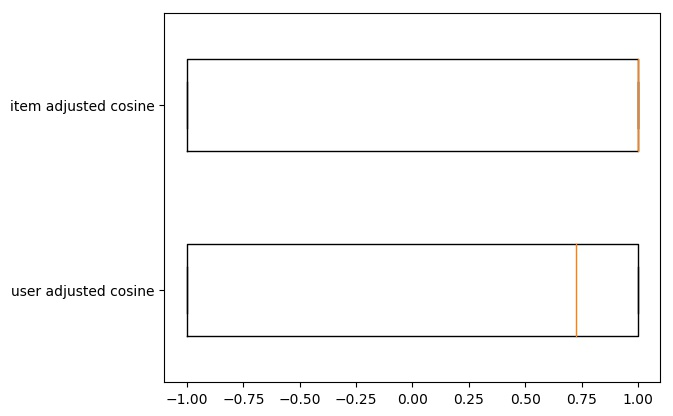
\includegraphics[width=0.8\textwidth]{chapter_4/boxplots/adjusted_cosine/adjusted_cosine_boxplot.jpg}
\caption{Adjusted Cosine Similarity Boxplot (Whiskers= -+1.5IQR)}
\label{figure:adjusted_cosine_similarity_boxplot}
\end{figure}

Adjusted cosine similarity seems to have distributed the values both for users and items very well.
There are no outliers for either of these boxplots. Although, items have at least 50\% of their
values at 1, users have at least 50\% of their values over 0.7. They both have their minimum
value at -1.

\begin{table}[H]
\centering
\caption{Adjusted Cosine Similarity Descriptive}
\label{table:adjusted_cosine_similarity_descriptive}
\begin{tabular}{|c|c|c|}
\hline
          & \textbf{users} & \textbf{items} \\ \hline
count     & 14547343       & 18578462       \\ \hline
mean      & 0.073856558    & 0.09784622     \\ \hline
std       & 0.9611564664   & 0.9793750112   \\ \hline
min       & -1             & -1             \\ \hline
25\%      & -1             & -1             \\ \hline
50\%      & 0.7255719661   & 1              \\ \hline
75\%      & 1              & 1              \\ \hline
max       & 1              & 1              \\ \hline
max count & 6998746        & 9729527        \\ \hline
min count & 5753489        & 7845237        \\ \hline
\end{tabular}
\end{table}

\begin{table}[H]
\centering
\caption{Adjusted Cosine Similarity Count Descriptive}
\label{adjusted_cosine_similarity_count_descriptive}
\begin{tabular}{|c|c|c|}
\hline
          & \textbf{users}  & \textbf{items} \\ \hline
count     & 38302           & 119634         \\ \hline
mean      & 759.6127095191  & 310.5883277329 \\ \hline
std       & 1179.0168839062 & 666.8475091836 \\ \hline
min       & 1               & 1              \\ \hline
25\%      & 45              & 39             \\ \hline
50\%      & 260             & 123            \\ \hline
75\%      & 968             & 340            \\ \hline
max       & 13798           & 30920          \\ \hline
max count & 1               & 1              \\ \hline
min count & 569             & 398            \\ \hline
\end{tabular}
\end{table}

\subsection{Modified Adjusted Cosine Similarity}

\begin{figure}[H]
\centering
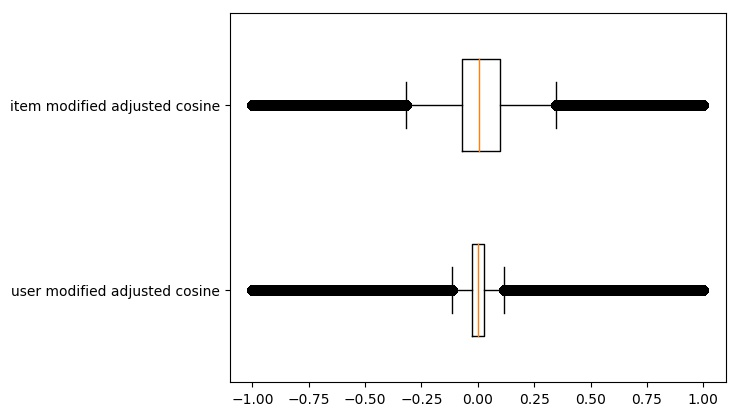
\includegraphics[width=0.8\textwidth]{chapter_4/boxplots/modified_adjusted_cosine/modified_adjusted_cosine_boxplot.jpg}
\caption{Modified Adjusted Cosine Similarity Boxplot (Whiskers= -+1.5IQR)}
\label{figure:modified_adjusted_cosine_similarity_boxplot}
\end{figure}

The modification used in adjusted cosine similarity seems to have enclosed the values near zero.
Their median is aligned very close to zero. The whiskers for items are around -0.4 and 0.4
for left and right respectively. For users, the whiskers are around -0.12 and 0.12 for left and right
respectively. Items similarities behave like a wider version of users similarities, probably
because items are more than twice the size of users which allows them to form a wider range of
different similarities.

\begin{table}[H]
\centering
\caption{Modified Adjusted Cosine Similarity Descriptive}
\label{table:modified_adjusted_cosine_similarity_descriptive}
\begin{tabular}{|c|c|c|}
\hline
          & \textbf{users} & \textbf{items} \\ \hline
count     & 14547343       & 18578462       \\ \hline
mean      & 0.0004873924   & 0.0165982167   \\ \hline
std       & 0.1313835099   & 0.398039276    \\ \hline
min       & -1             & -1             \\ \hline
25\%      & -0.0280684821  & -0.0701974943  \\ \hline
50\%      & 0.0012377237   & 0.0033406502   \\ \hline
75\%      & 0.029188451    & 0.096874534    \\ \hline
max       & 1              & 1              \\ \hline
max count & 17005          & 863028         \\ \hline
min count & 11891          & 679602         \\ \hline
\end{tabular}
\end{table}

\begin{table}[H]
\centering
\caption{Modified Adjusted Cosine Similarity Count Descriptive}
\label{table:modified_adjusted_cosine_similarity_count_descriptive}
\begin{tabular}{|c|c|c|}
\hline
          & \textbf{users}  & \textbf{items} \\ \hline
count     & 38302           & 119634         \\ \hline
mean      & 759.6127095191  & 310.5883277329 \\ \hline
std       & 1179.0168839062 & 666.8475091836 \\ \hline
min       & 1               & 1              \\ \hline
25\%      & 45              & 39             \\ \hline
50\%      & 260             & 123            \\ \hline
75\%      & 968             & 340            \\ \hline
max       & 13798           & 30920          \\ \hline
max count & 1               & 1              \\ \hline
min count & 569             & 398            \\ \hline
\end{tabular}
\end{table}

\subsection{Pearson Correlation Coefficient}

\begin{figure}[H]
\centering
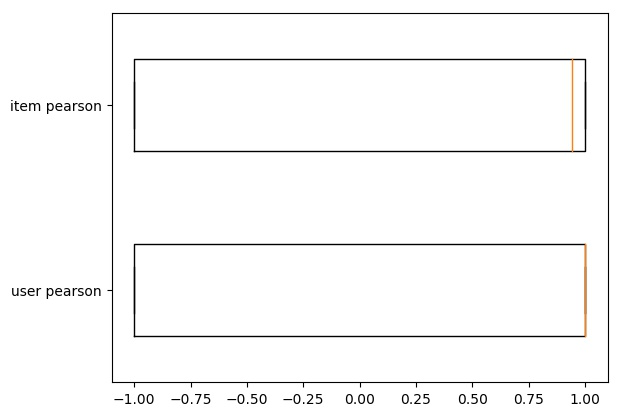
\includegraphics[width=0.8\textwidth]{chapter_4/boxplots/pearson/pearson_boxplot.jpg}
\caption{Pearson Correlation Coefficient Boxplot (Whiskers= -+1.5IQR)}
\label{figure:pearson_corr_coef_boxplot}
\end{figure}

The similarities formed using the Pearson correlation coefficient seem well distributed across
the range -1 to 1. No outliers exist in both users and items. In the users' boxplot at least 50\% of the
values appear to be near 1. In the items' boxplot at least 50\% of the values are over 0.8. The
minimum value for both of the similarities is at -1.

\begin{table}[H]
\centering
\caption{Pearson Correlation Coefficient Descriptive}
\label{table:pearson_corr_coef_descriptive}
\begin{tabular}{|c|c|c|}
\hline
          & \textbf{users} & \textbf{items} \\ \hline
count     & 12801832       & 9114131        \\ \hline
mean      & 0.2437009881   & 0.0973284577   \\ \hline
std       & 0.9285318435   & 0.9625193963   \\ \hline
min       & -1             & -1             \\ \hline
25\%      & -1             & -1             \\ \hline
50\%      & 1              & 0.940706152    \\ \hline
75\%      & 1              & 1              \\ \hline
max       & 1              & 1              \\ \hline
max count & 6825146        & 4489219        \\ \hline
min count & 4163467        & 3678485        \\ \hline
\end{tabular}
\end{table}

\begin{table}[H]
\centering
\caption{Pearson Correlation Coefficient Count Descriptive}
\label{table:pearson_corr_coef_boxplot}
\begin{tabular}{|c|c|c|}
\hline
          & \textbf{users}  & \textbf{items} \\ \hline
count     & 26166           & 40409          \\ \hline
mean      & 978.5089046855  & 451.0941126977 \\ \hline
std       & 1227.2905909627 & 753.2523780236 \\ \hline
min       & 1               & 1              \\ \hline
25\%      & 148             & 90             \\ \hline
50\%      & 507             & 222            \\ \hline
75\%      & 1353            & 500            \\ \hline
max       & 12486           & 17515          \\ \hline
max count & 1               & 1              \\ \hline
min count & 89              & 16             \\ \hline
\end{tabular}
\end{table}

\subsection{Pearson Modification 1}

\begin{figure}[H]
\centering
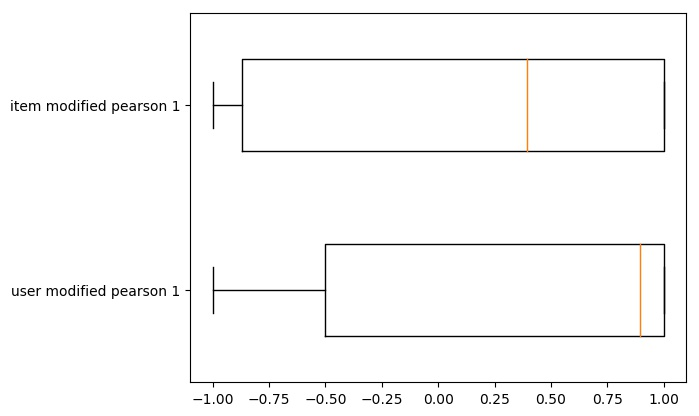
\includegraphics[width=0.8\textwidth]{chapter_4/boxplots/modified_pearson_1/modified_pearson_1_boxplot.jpg}
\caption{Modified Pearson 1 Boxplot (Whiskers= -+1.5IQR)}
\label{figure:modified_pearson_1_boxplot}
\end{figure}

The minimum value for both users and items similarities is at -1. Users have at least 50\% of their
values over 0.8 and at least 25\% at 1. Items' median is around 0.4. Items also seem to have
a 25\% of their value at 1. Both have their minimum at -1. At least 25\% of the similarities
for both users and items are negative.

\begin{table}[H]
\centering
\caption{Modified Pearson 1 Descriptive}
\label{table:modified_pearson_1_descriptive}
\begin{tabular}{|c|c|c|}
\hline
          & \textbf{users} & \textbf{items} \\ \hline
count     & 1161526        & 560066         \\ \hline
mean      & 0.3619158933   & 0.1343440987   \\ \hline
std       & 0.8153387654   & 0.8305601334   \\ \hline
min       & -1             & -1             \\ \hline
25\%      & -0.5           & -0.8703882798  \\ \hline
50\%      & 0.8947368421   & 0.3942210015   \\ \hline
75\%      & 1              & 1              \\ \hline
max       & 1              & 1              \\ \hline
max count & 529709         & 184408         \\ \hline
min count & 227880         & 133046         \\ \hline
\end{tabular}
\end{table}

\begin{table}[H]
\centering
\caption{Modified Pearson 1 Count Descriptive}
\label{modified_pearson_1_count_descriptive}
\begin{tabular}{|c|c|c|}
\hline
          & \textbf{users} & \textbf{items} \\ \hline
count     & 19566          & 25208          \\ \hline
mean      & 118.7290197281 & 44.4355760076  \\ \hline
std       & 266.6999446542 & 153.5700823656 \\ \hline
min       & 1              & 1              \\ \hline
25\%      & 5              & 2              \\ \hline
50\%      & 23             & 6              \\ \hline
75\%      & 105            & 24             \\ \hline
max       & 5003           & 5401           \\ \hline
max count & 1              & 1              \\ \hline
min count & 2066           & 5234           \\ \hline
\end{tabular}
\end{table}


\subsection{Pearson Modification 2}
\begin{figure}[H]
\centering
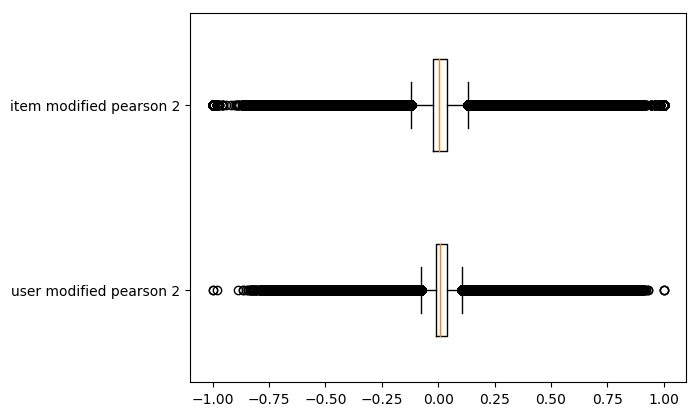
\includegraphics[width=0.8\textwidth]{chapter_4/boxplots/modified_pearson_2/modified_pearson_2_boxplot.jpg}
\caption{Modified Pearson 2 Boxplot (Whiskers= -+1.5IQR)}
\label{figure:modified_pearson_2_boxplot}
\end{figure}

At a first glance, these boxplots look very similar to \autoref{figure:modified_adjusted_cosine_similarity_boxplot}.
This is probably because the modification in both cases was to include the entire vectors in the
denominator (see \autoref{eq:modified_adjusted_cosine} and \autoref{eq:pearson_2}). Both boxplots have
their median near zero. They both have many outliers that spread both left and right of the boxes with
minimum value at -1 and maximum at 1. The whiskers are around -0.2 to -0.15 from the left
side and 0.15 to 0.2 from the right side.

\begin{table}[H]
\centering
\caption{Modified Pearson 2 Descriptive}
\label{table:modified_pearson_2_descriptive}
\begin{tabular}{|c|c|c|}
\hline
          & \textbf{users} & \textbf{items} \\ \hline
count     & 12801832       & 9114131        \\ \hline
mean      & 0.0218434042   & 0.0101521404   \\ \hline
std       & 0.089326644    & 0.1385987076   \\ \hline
min       & -1             & -1             \\ \hline
25\%      & -0.0093795851  & -0.0251329949  \\ \hline
50\%      & 0.0076098072   & 0.0037092894   \\ \hline
75\%      & 0.0367446145   & 0.0372677996   \\ \hline
max       & 1              & 1              \\ \hline
max count & 3              & 710            \\ \hline
min count & 2              & 412            \\ \hline
\end{tabular}
\end{table}

\begin{table}[H]
\centering
\caption{Modified Pearson 2 Count Descriptive}
\label{table:modified_pearson_2_count_descriptive}
\begin{tabular}{|c|c|c|}
\hline
          & \textbf{users}  & \textbf{items} \\ \hline
count     & 26166           & 40409          \\ \hline
mean      & 978.5089046855  & 451.0941126977 \\ \hline
std       & 1227.2905909627 & 753.2523780236 \\ \hline
min       & 1               & 1              \\ \hline
25\%      & 148             & 90             \\ \hline
50\%      & 507             & 222            \\ \hline
75\%      & 1353            & 500            \\ \hline
max       & 12486           & 17515          \\ \hline
max count & 1               & 1              \\ \hline
min count & 89              & 16             \\ \hline
\end{tabular}
\end{table}

\subsection{MSD}
\begin{figure}[H]
\centering
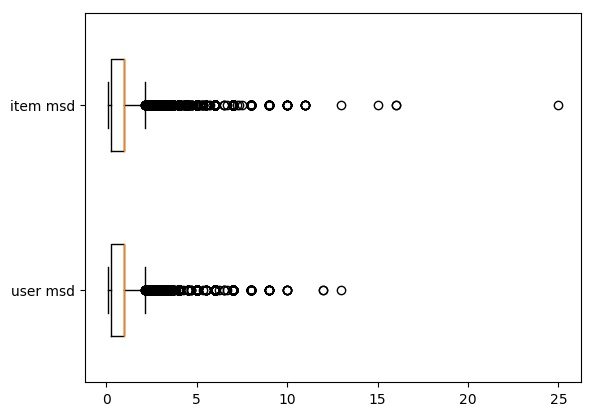
\includegraphics[width=0.8\textwidth]{chapter_4/boxplots/msd/msd_boxplot.jpg}
\caption{MSD Boxplot (Whiskers= -+1.5IQR)}
\label{figure:msd_boxplot}
\end{figure}

The minimum similarity value for both users and items is very close to zero. Their median
is around 1 and 75\% of the similarities are below 2. They both have a lot of outliers that
reach a score around 15. Item similarity has some more extreme outliers that are very close to 25.

\begin{table}[H]
\centering
\caption{MSD Descriptive}
\label{table:msd_descriptive}
\begin{tabular}{|c|c|c|}
\hline
          & \textbf{users} & \textbf{items} \\ \hline
count     & 9805108        & 12434536       \\ \hline
mean      & 0.6661864961   & 0.6544694584   \\ \hline
std       & 0.5256923021   & 0.4628208708   \\ \hline
min       & 0.0625         & 0.0625         \\ \hline
25\%      & 0.25           & 0.25           \\ \hline
50\%      & 1              & 1              \\ \hline
75\%      & 1              & 1              \\ \hline
max       & 13             & 25             \\ \hline
max count & 1              & 1              \\ \hline
min count & 598720         & 800571         \\ \hline
\end{tabular}
\end{table}

\begin{table}[H]
\centering
\caption{MSD Count Descriptive}
\label{msd_count_descriptive}
\begin{tabular}{|c|c|c|}
\hline
          & \textbf{users} & \textbf{items} \\ \hline
count     & 38442          & 120382         \\ \hline
mean      & 510.1247593778 & 206.5846388995 \\ \hline
std       & 850.5223750077 & 484.7004513454 \\ \hline
min       & 1              & 1              \\ \hline
25\%      & 25             & 22             \\ \hline
50\%      & 156            & 72             \\ \hline
75\%      & 613            & 213            \\ \hline
max       & 11014          & 23589          \\ \hline
max count & 1              & 1              \\ \hline
min count & 1182           & 1563           \\ \hline
\end{tabular}
\end{table}

\subsection{MAD}

\begin{figure}[H]
\centering
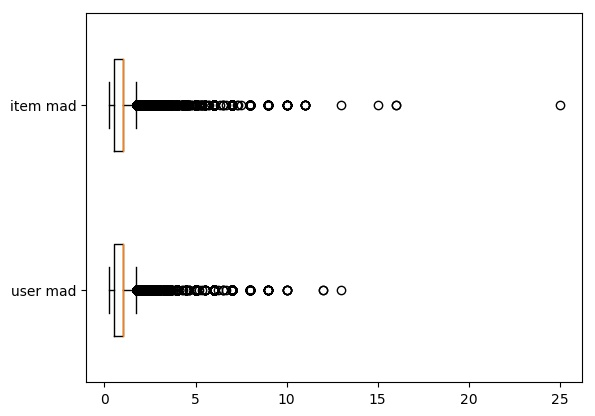
\includegraphics[width=0.8\textwidth]{chapter_4/boxplots/mad/mad_boxplot.jpg}
\caption{MAD Boxplot (Whiskers= -+1.5IQR)}
\label{figure:mad_boxplot}
\end{figure}

As expected, mean absolute difference boxplots are very similar to that of mean squared difference
\autoref{figure:msd_boxplot}. It is clear that the boxes have shrunk, due to the
fact that MAD uses the absolute values instead of the squared ones and this modification
lowers the standard deviation between the similarities.

\begin{table}[H]
\centering
\caption{MAD Descriptive}
\label{table:mad_descriptive}
\begin{tabular}{|c|c|c|}
\hline
          & \textbf{users} & \textbf{items} \\ \hline
count     & 9805108        & 12434536       \\ \hline
mean      & 0.7962500349   & 0.7668765592   \\ \hline
std       & 0.4338056858   & 0.3639417506   \\ \hline
min       & 0.25           & 0.25           \\ \hline
25\%      & 0.5            & 0.5            \\ \hline
50\%      & 1              & 1              \\ \hline
75\%      & 1              & 1              \\ \hline
max       & 13             & 25             \\ \hline
max count & 1              & 1              \\ \hline
min count & 598720         & 800571         \\ \hline
\end{tabular}
\end{table}

\begin{table}[H]
\centering
\caption{MAD Count Descriptive}
\label{table:mad_count_descriptive}
\begin{tabular}{|c|c|c|}
\hline
          & users          & items          \\ \hline
count     & 38442          & 120382         \\ \hline
mean      & 510.1247593778 & 206.5846388995 \\ \hline
std       & 850.5223750077 & 484.7004513454 \\ \hline
min       & 1              & 1              \\ \hline
25\%      & 25             & 22             \\ \hline
50\%      & 156            & 72             \\ \hline
75\%      & 613            & 213            \\ \hline
max       & 11014          & 23589          \\ \hline
max count & 1              & 1              \\ \hline
min count & 1182           & 1563			\\ \hline
\end{tabular}
\end{table}

\subsection{Jaccard Coefficient}
\begin{figure}[H]
\centering
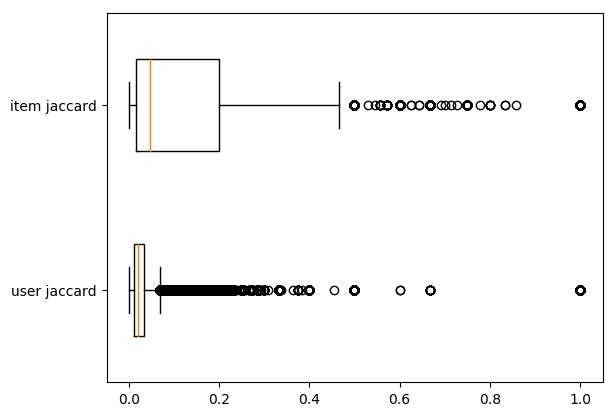
\includegraphics[width=0.8\textwidth]{chapter_4/boxplots/jaccard/jaccard_boxplot.jpg}
\caption{Jaccard Boxplot (Whiskers= -+1.5IQR)}
\label{figure:jaccard_boxplot}
\end{figure}

Both item and user similarity values have a minimum value near zero. The items' right whisker value is
around 0.45 and for the users around 0.04. Both items and users similarity outliers appear to reach the value
1. Also the number of outliers in item cosine seems significantly lower than users. At least 75\% of
users similarities are lower than 0.1. In contrast, at least 25\% of item similarities are larger than 0.2.
Users' boxplot is very narrow which indicates that 50\% of the values are very close to each other. It
covers a range of merely 0.02. On the other hand, the items' boxplot is relatively wider. It covers a range of about 0.19,
which confirms the wider spread of the values.

\begin{table}[H]
\centering
\caption{Jaccard Descriptive}
\label{table:jaccard_descriptive}
\begin{tabular}{|c|c|c|}
\hline
          & \textbf{users} & \textbf{items} \\ \hline
count     & 14614164       & 18672616       \\ \hline
mean      & 0.0307346429   & 0.1733928584   \\ \hline
std       & 0.0544456926   & 0.2779653358   \\ \hline
min       & 0.0006485084   & 0.0006060606   \\ \hline
25\%      & 0.0112359551   & 0.0153846154   \\ \hline
50\%      & 0.0196078431   & 0.0476190476   \\ \hline
75\%      & 0.0344827586   & 0.2            \\ \hline
max       & 1              & 1              \\ \hline
max count & 26746          & 1522328        \\ \hline
min count & 1              & 1              \\ \hline
\end{tabular}
\end{table}

\begin{table}[H]
\centering
\caption{Jaccard Count Descriptive}
\label{table:jaccard_count_descriptive}
\begin{tabular}{|c|c|c|}
\hline
          & \textbf{users}  & \textbf{items} \\ \hline
count     & 39156           & 121140         \\ \hline
mean      & 746.4584737971  & 308.281591547  \\ \hline
std       & 1174.5013754664 & 666.5799806645 \\ \hline
min       & 1               & 1              \\ \hline
25\%      & 40              & 37             \\ \hline
50\%      & 246             & 120            \\ \hline
75\%      & 944             & 338            \\ \hline
max       & 13843           & 31057          \\ \hline
max count & 1               & 1              \\ \hline
min count & 793             & 545            \\ \hline
\end{tabular}
\end{table}


\section{Evaluation Metrics}
The accuracy of the predictions is one of the most important goals in recommender
systems as it gives more chances that the prediction will be relevant to the
user. As discussed in \autoref{chap:1} other goals include the novelty of the
recommendations, serendipity and diversity. In this thesis the focus is
on the accuracy of the predictions. Four metrics will be discussed to evaluate the
Recursive Nearest Neighbors algorithm on the Epinions dataset.
\subsection{Root Mean Squared Error (RMSE)}
RMSE is one of the most popular accuracy estimators.
It sums the squared error between the true and estimated value divided by the
number of the predictions the model was able to extract. Finally it is square
rooted so that the error corresponds to units of ratings instead of square
units. \citep{Ricci}
$$RMSE = \sqrt{\frac{\sum_{(u,i) \in \mathcal{T}(r_{u,i} - \hat{r}_{u,i})^2}}{n}}$$
where,
\begin{itemize}
	\item[] $\mathcal{T}$ is the test set
	\item[] $r_{u,i}$ is the true rating of user $u$ to item $i$ in $\mathcal{T}$
	\item[] $\hat{r}_{u,i}$ is the rating prediction for user $u$ to item $i$
	\item[] $n$ is the number of predictions
\end{itemize}

\subsection{Mean Absolute Error (MAE)}
MAE is another popular metric for accuracy estimation. It sums the absolute
value between the difference between the true and estimated ratings
divided by the number of predictions. \citep{Ricci}
$$MAE = \frac{\sum_{(u,i) \in \mathcal{T}\left|r_{u,i} - \hat{r}_{u,i}\right|}}{n}$$
where,
\begin{itemize}
	\item[] $\mathcal{T}$ is the test set
	\item[] $r_{u,i}$ is the true rating of user $u$ to item $i$ in $\mathcal{T}$
	\item[] $\hat{r}_{u,i}$ is the rating prediction for user $u$ to item $i$
	\item[] $n$ is the number of predictions
\end{itemize}

\subsection{Mean Absolute User Error (MAUE)}
While RMSE and MAE estimate the global error to the system MAUE first
calculates the MAE score for each user then averages all user errors to find
how much the system diverges on average from each user \citep{Massa}.
$$MAUE = \frac{1}{n}\sum_{u \in \mathcal{T}}\frac{\sum_{i \in \mathcal{I}_u\mathopen|r_{u,i} - \hat{r}_{u,i}\mathclose|}}{n_u}$$
where,
\begin{itemize}
	\item[] $\mathcal{T}$ is the test set
	\item[] $r_{u,i}$ is the true rating of user $u$ to item $i$ in $\mathcal{T}$
	\item[] $\hat{r}_{u,i}$ is the rating prediction for user $u$ to item $i$
	\item[] $n_u$ is the number of predictions for user $u$
	\item[] $n$ is the number of users for whom predictions were made for
\end{itemize}
\subsection{Root Mean Squared User Error (RMSUE)}
Like in MAUE, the equation for RMSE can be used to produce a per user rmse estimate.
In this metric first the RMSE for every user is computed. Then the RMSEs of
the users are averaged to form the RMSUE score with is an estimate in the
error of the model per user of the dataset.
$$RMSUE = \frac{1}{n}\sum_{u \in \mathcal{T}}\sqrt{\frac{\sum_{i \in \mathcal{I}_u(y_{u,i} - \hat{y}_{u,i})^2}}{n_u}}$$
where,
\begin{itemize}
	\item[] $\mathcal{T}$ is the test set
	\item[] $r_{u,i}$ is the true rating of user $u$ to item $i$ in $\mathcal{T}$
	\item[] $\hat{r}_{u,i}$ is the rating prediction for user $u$ to item $i$
	\item[] $n_u$ is the number of predictions for user $u$
	\item[] $n$ is the number of users for whom predictions were made for
\end{itemize}

\section{Evaluation Results and Benchmarks}\label{sec:4.3}
For this experiment item-based and user-based similarities discussed in \autoref{chap:2} where used.
Any similarity metrics that could contain
negative similarities, had those negative similarities excluded from the
computations.
For the K-Nearest Neighbors, the following 22 different values
of $\mathcal{K}$ were used:
$$\mathcal{K} = [1, 3, 5, 10, 15, 20, 25, 30, 35, 40, 45, 50, 55, 60, 65, 70, 75, 80, 85, 90, 95, 100]$$
For the Recursive K-Nearest Neighbors, as defined in the
algorithmic steps of \autoref{chap:3}, 22 different values of $\mathcal{M}$
were also used:
$$\mathcal{M} = [1, 3, 5, 10, 15, 20, 25, 30, 35, 40, 45, 50, 55, 60, 65, 70, 75, 80, 85, 90, 95, 100]$$

Below, the best outcome based on each evaluation metric for user-based and
item-based CF will be presented. The combined errors for KNN and Recursive-KNN
for RMSE and MAE below are computed using these formulas:
\begin{itemize}
	\item[] \textbf{Total RMSE:}
	$$RMSE_{Total} = \sqrt{\frac{n_{KNN}*RMSE_{KNN}^2 + n_{R-KNN}*RMSE_{R-KNN}^2}{n_{KNN} + n_{R-KNN}}}$$
	where,
	\begin{itemize}
		\item[] $n_{KNN}$ is the number of predictions made using the KNN algorithm
		\item[] $RMSE_{KNN}$ is the RMSE score using the KNN algorithm
		\item[] $n_{R-KNN}$ is the number of predictions made using the Recursive KNN algorithm
		\item[] $RMSE_{R-KNN}$ is the RMSE score using the Recursive KNN algorithm
	\end{itemize}
	\item[] \textbf{Total MAE:}
	$$MAE_{Total} = \frac{n_{KNN}*MAE_{KNN} + n_{R-KNN}*MAE_{R-KNN}}{n_{KNN} + n_{R-KNN}}$$
	where,
	\begin{itemize}
		\item[] $n_{KNN}$ is the number of predictions made using the KNN algorithm
		\item[] $MAE_{KNN}$ is the MAE score using the KNN algorithm
		\item[] $n_{R-KNN}$ is the number of predictions made using the Recursive KNN algorithm
		\item[] $MAE_{R-KNN}$ is the MAE score using the Recursive KNN algorithm
	\end{itemize}
\end{itemize}

\autoref{chap:appendix_src} has a link to
the code written in Python(version 3.6) using the Anaconda distribution \citep{anaconda}
that calculated the similarities, rating predictions
and the errors. It also contains the train and test data, the \LaTeX{} structure
that this thesis was build on and the numerical results.
\autoref{chap:appendix_results} contains all the plots produced by the
numerical results. All plots in this thesis were produced using the Matplotlib library
\citep{Hunter:2007}.

\subsection{User-Based}
\begin{figure}[H]
\centering
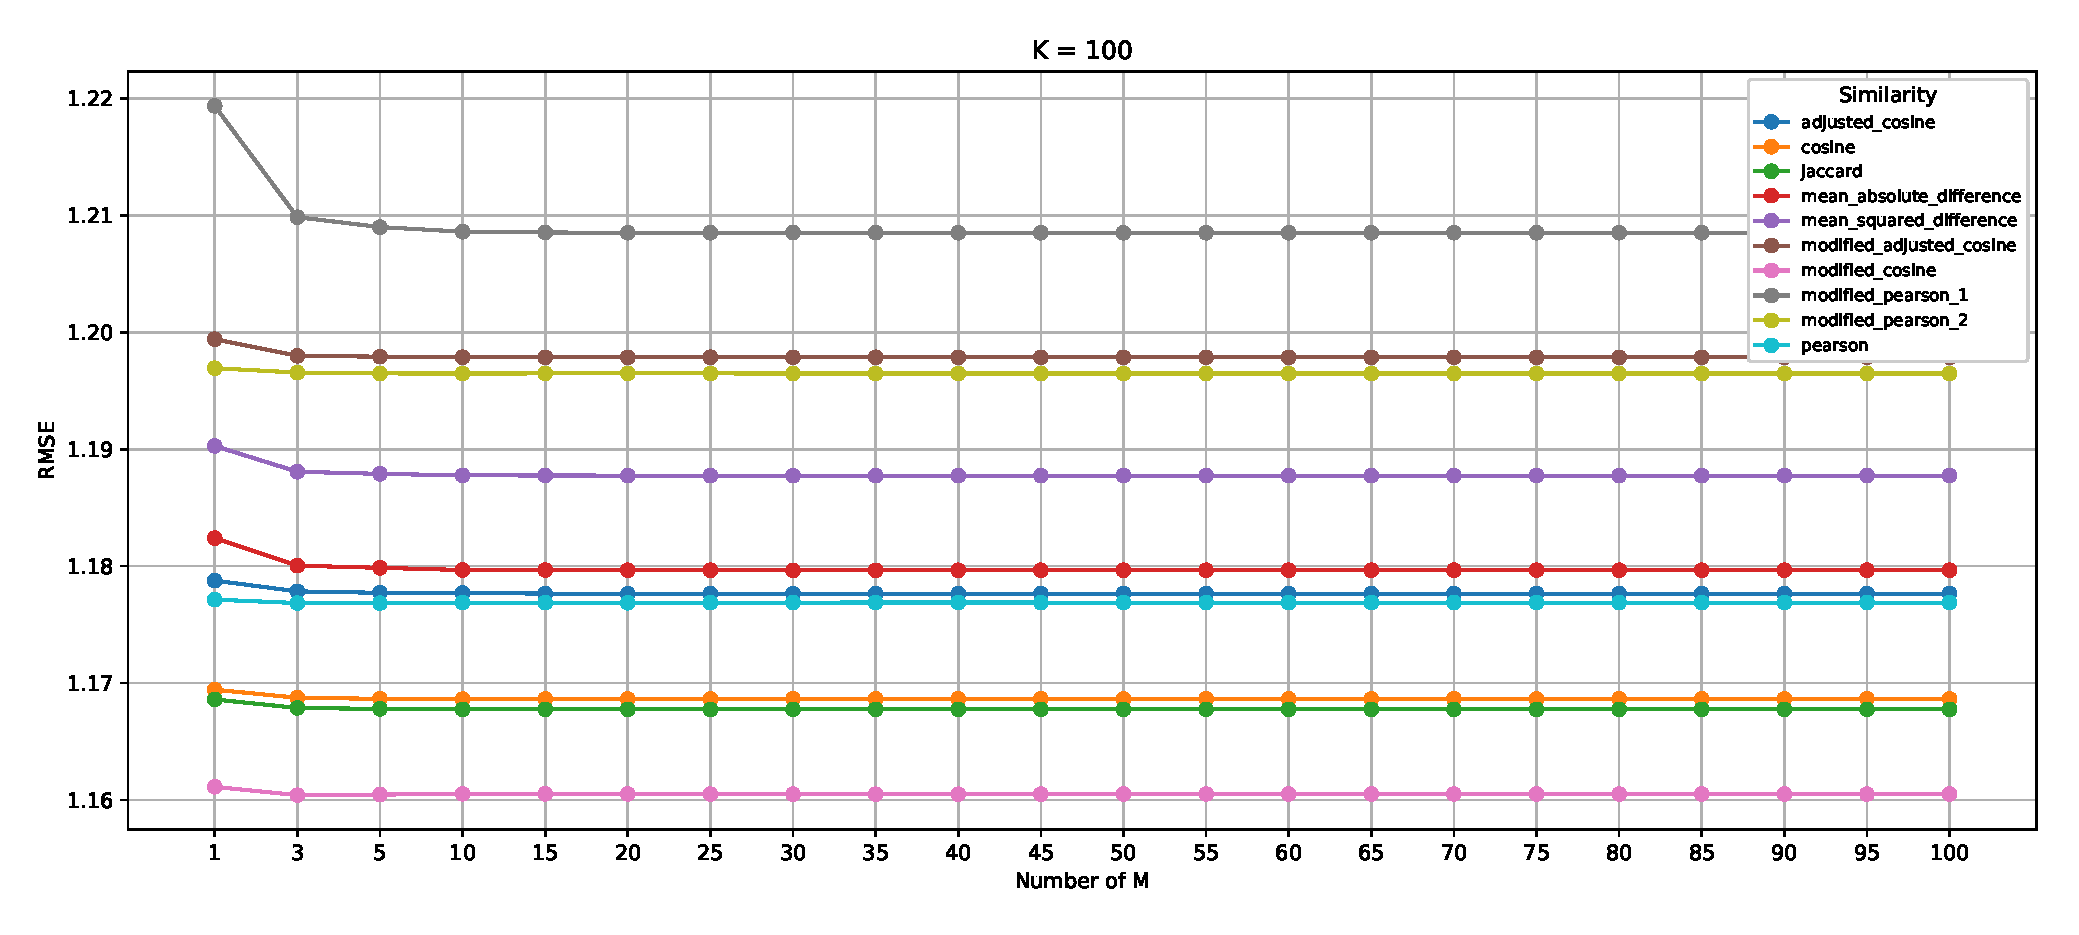
\includegraphics[width=1\textwidth]{chapter_4/evaluation/evaluation_user_rmse.eps}
\caption{User-based Total RMSE Best Score}
\label{figure:user_best_total_rmse}
\end{figure}
The best RMSE score for user-based CF was produced using $\mathcal{K}=100$ and $\mathcal{M}=3$.
The exact RMSE score is 1.1604146071 and it was calculated based on 124433 rating predictions(\autoref{table:prediction_counters_by_sim})
using the modified cosine similarity(\autoref{eq:modified_cosine})
for the 144621 ratings in the test set(\autoref{table:epinions_descriptive}).

\begin{figure}[H]
\centering
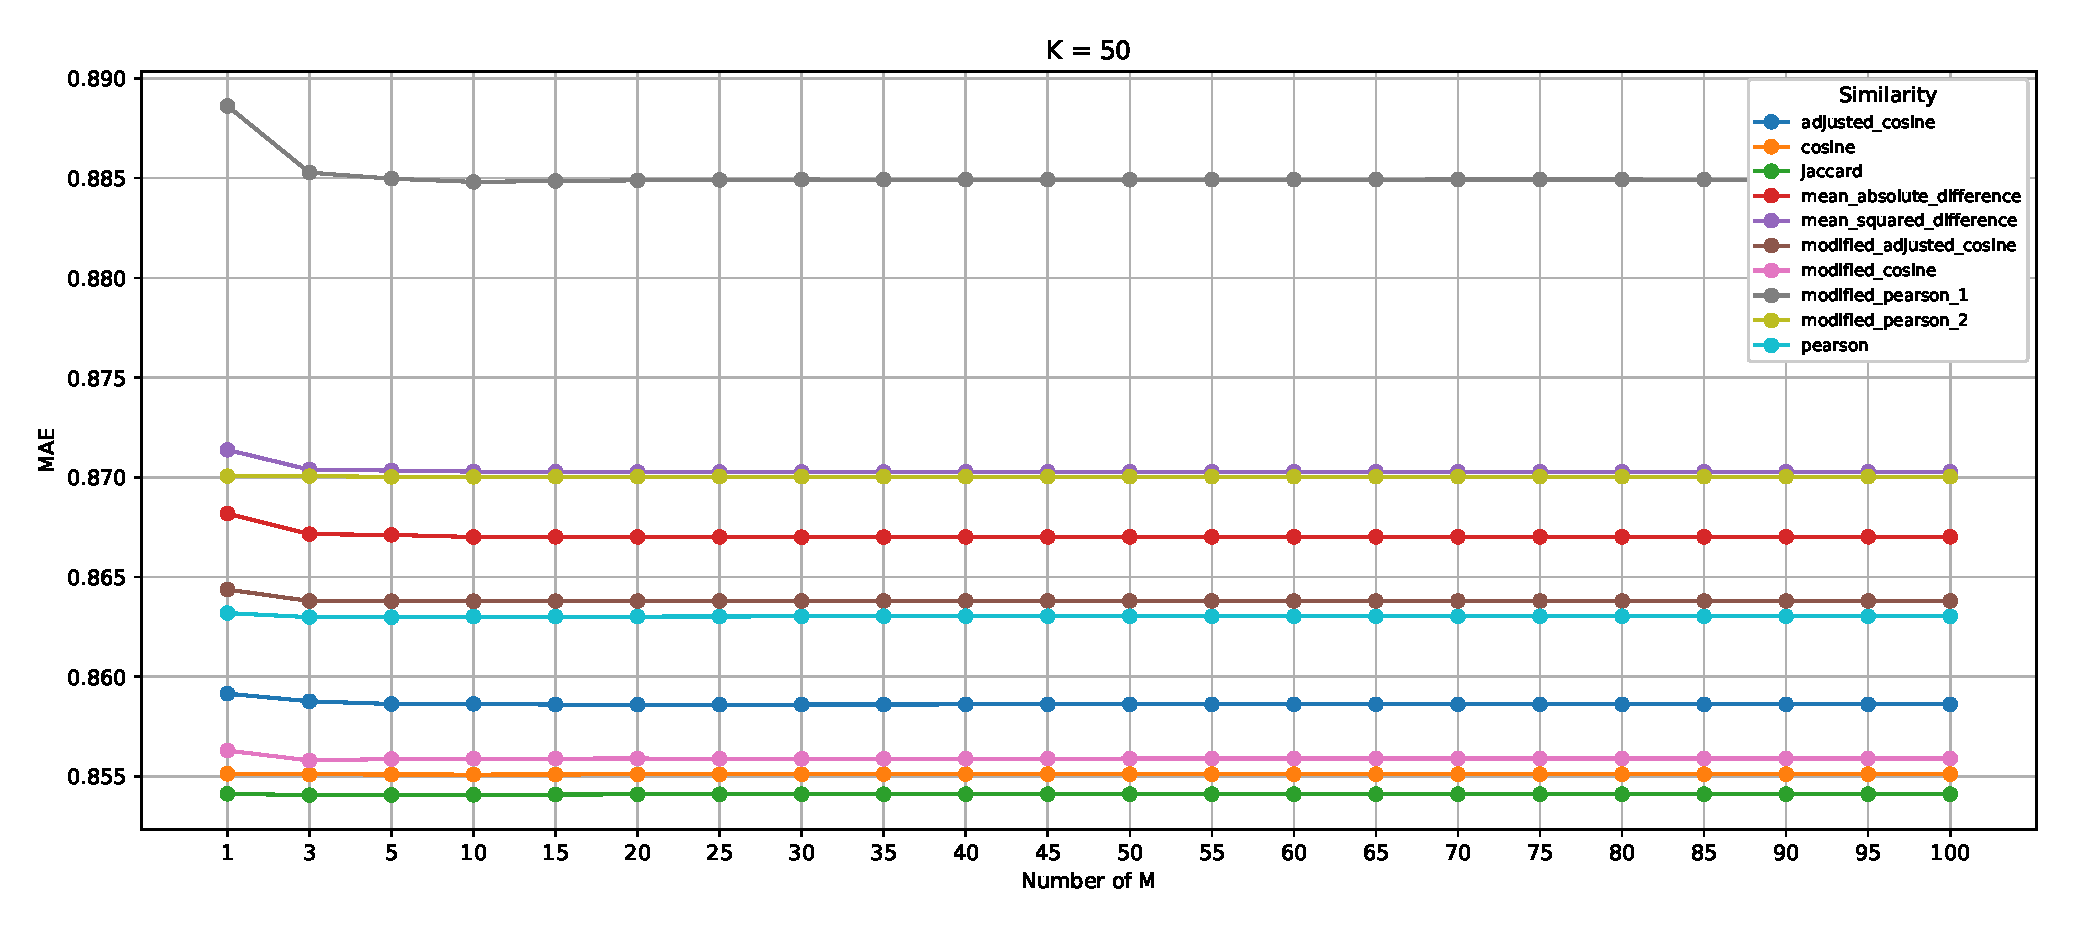
\includegraphics[width=1\textwidth]{chapter_4/evaluation/evaluation_user_mae.eps}
\caption{User-based Total MAE Best Score}
\label{figure:user_total_mae}
\end{figure}

The best MAE score for user-based CF was produced using $\mathcal{K}=50$ and $\mathcal{M}=3$.
The exact MAE score is 0.854066176 and it was calculated based on 124433 rating predictions(\autoref{table:prediction_counters_by_sim})
using the jaccard coefficient(\autoref{eq:jaccard})
for the 144621 ratings in the test set(\autoref{table:epinions_descriptive}).

\begin{figure}[H]
\centering
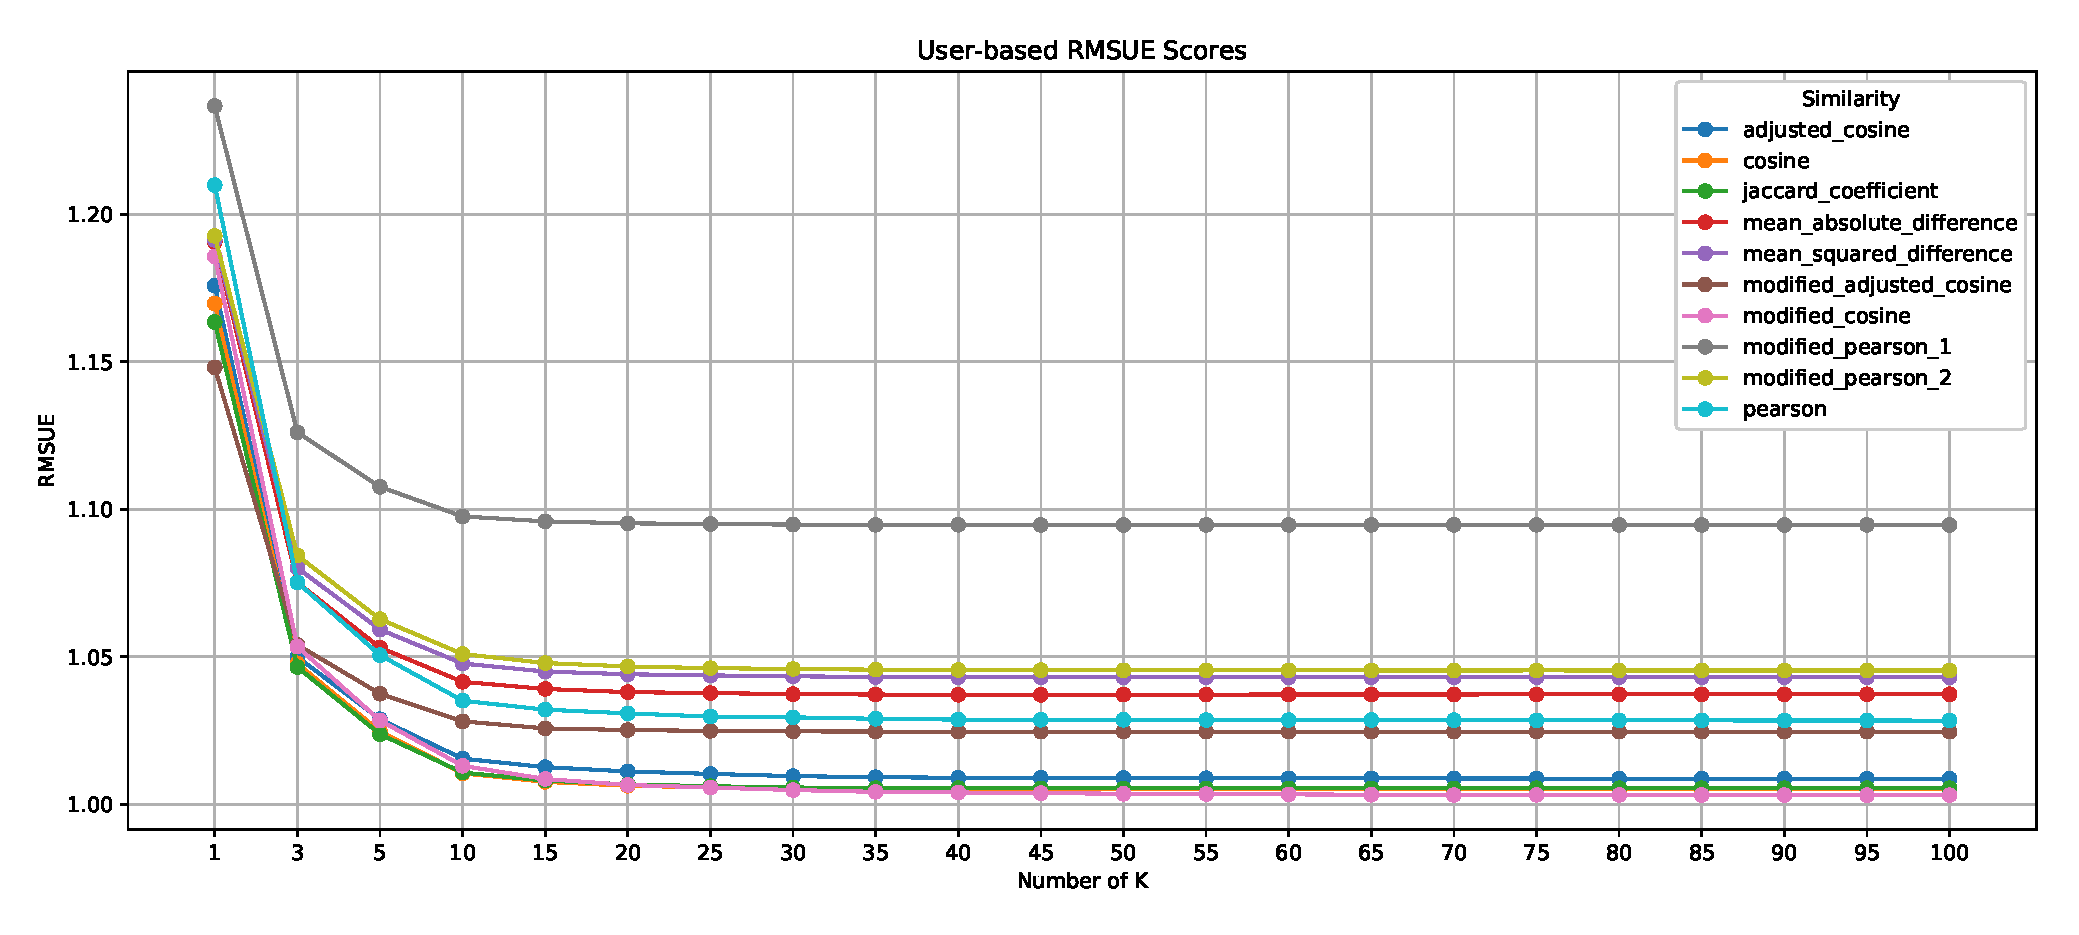
\includegraphics[width=1\textwidth]{chapter_4/knn/User_RMSUE_KNN.eps}
\caption{User-based KNN RMSUE Scores}
\label{figure:User_knn_rmsue}
\end{figure}

The best KNN RMSUE score for user-based CF was produced using $\mathcal{K}=100$.
The exact KNN RMSUE score is 1.0031145695 and it was calculated based on 100311 rating
predictions(\autoref{table:prediction_counters_by_sim})
using the modified cosine similarity(\autoref{eq:modified_cosine})
for the 144621 ratings in the test set(\autoref{table:epinions_descriptive}).

\begin{figure}[H]
\centering
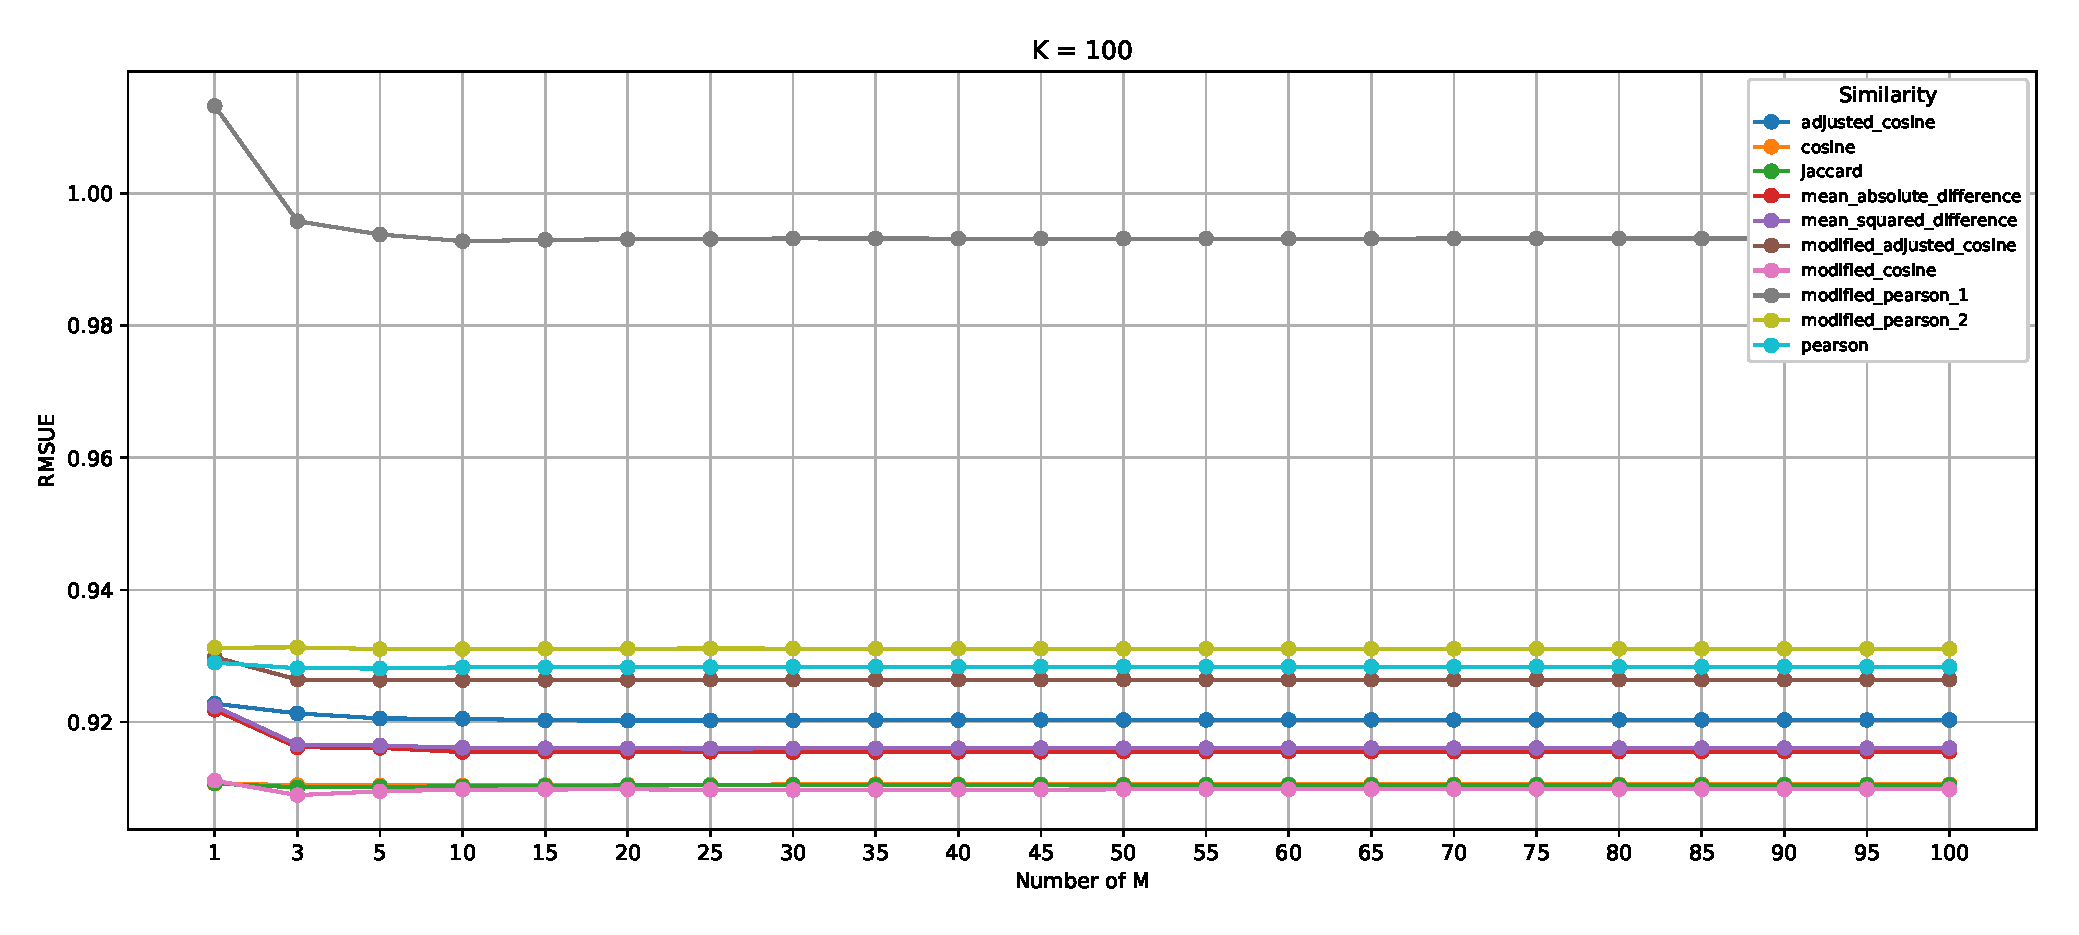
\includegraphics[width=1\textwidth]{chapter_4/evaluation/evaluation_user_rmsue.eps}
\caption{User-based Recursive-KNN RMSUE Best Score}
\label{figure:User_rknn_rmsue}
\end{figure}

The best Recursive-KNN RMSUE score for user-based CF was produced using $\mathcal{K}=100$ and $\mathcal{M}=3$.
The exact Recursive-KNN RMSUE score is 0.9089525549 and it was calculated based on 24122 rating
predictions(\autoref{table:prediction_counters_by_sim})
using the modified cosine similarity(\autoref{eq:modified_cosine})
out of the 25061 pairs for which KNN was unable to find neighbors(\autoref{table:users_log}).

\begin{figure}[H]
\centering
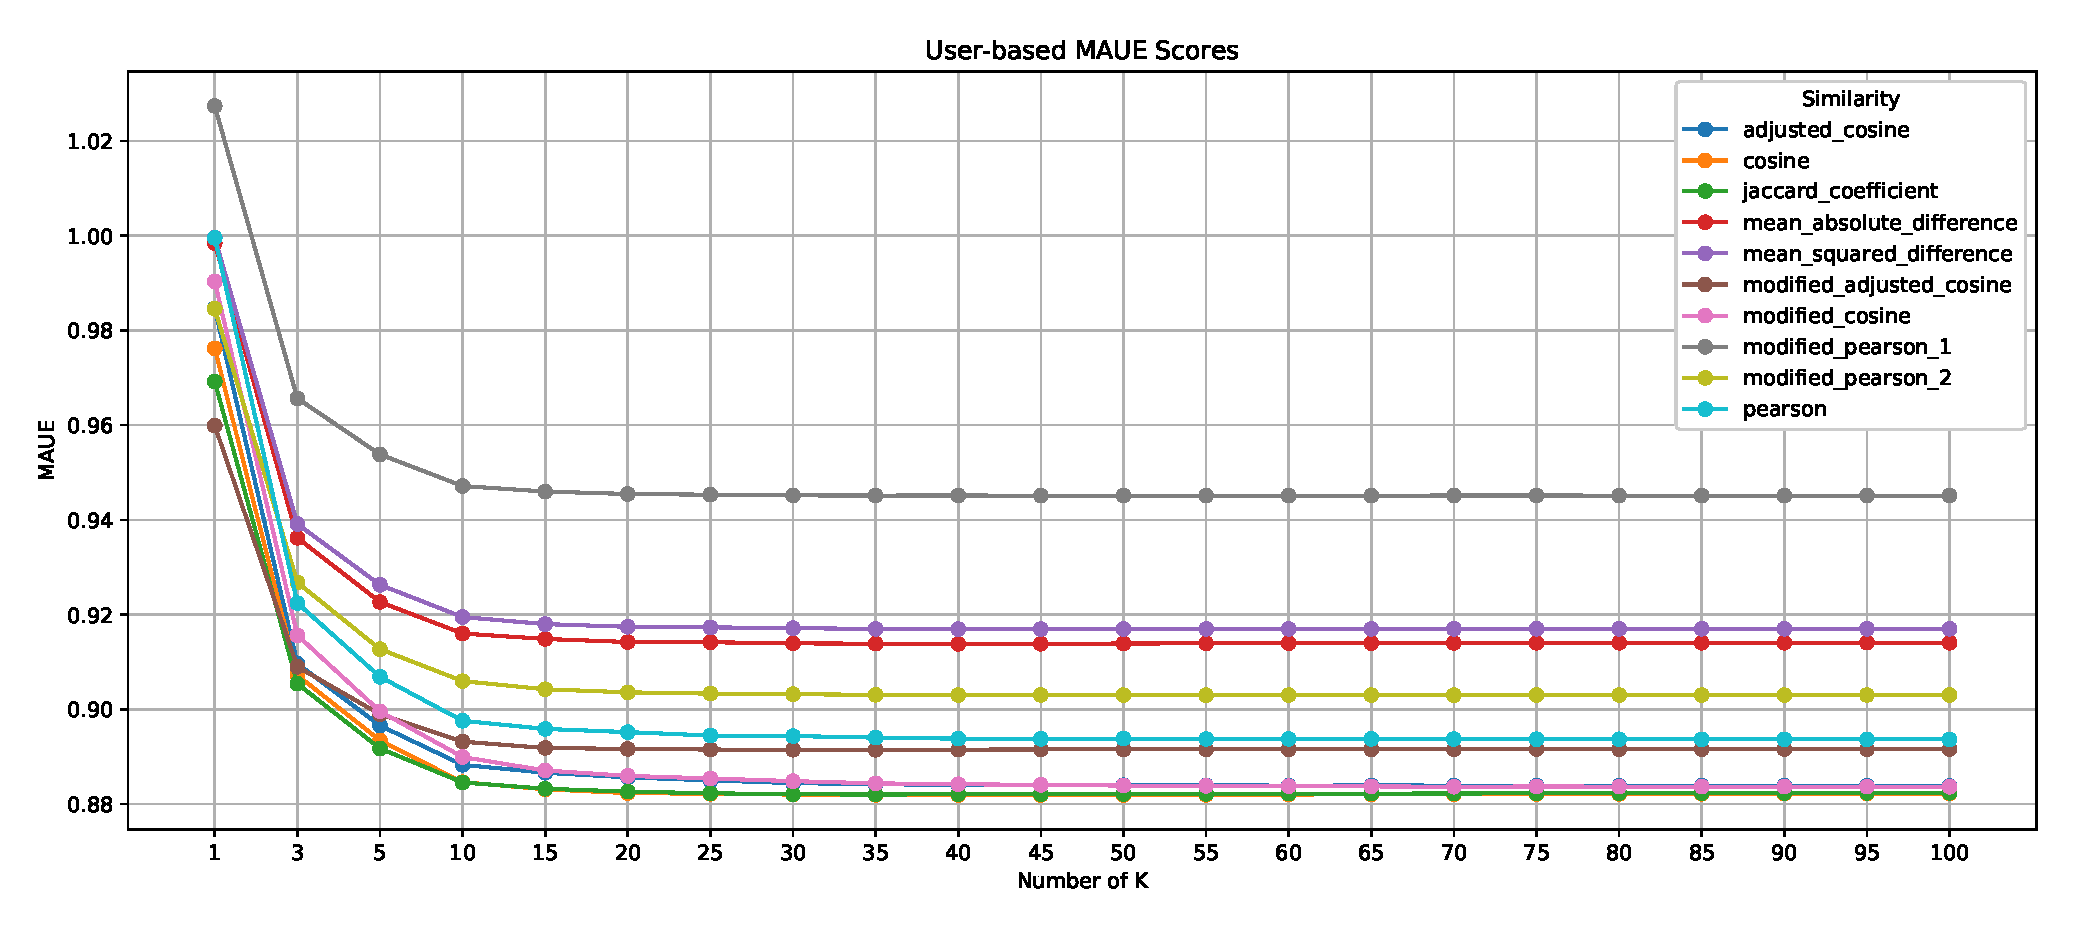
\includegraphics[width=1\textwidth]{chapter_4/knn/User_MAUE_KNN.eps}
\caption{User-based KNN MAUE Scores}
\label{figure:User_knn_maue}
\end{figure}

The best KNN MAUE score for user-based CF was produced using $\mathcal{K}=50$.
The exact KNN MAUE score is 0.8819077974 and it was calculated based on 100311 rating predictions(\autoref{table:prediction_counters_by_sim})
using the cosine similarity(\autoref{eq:cosine})
for the 144621 ratings in the test set(\autoref{table:epinions_descriptive}).

\begin{figure}[H]
\centering
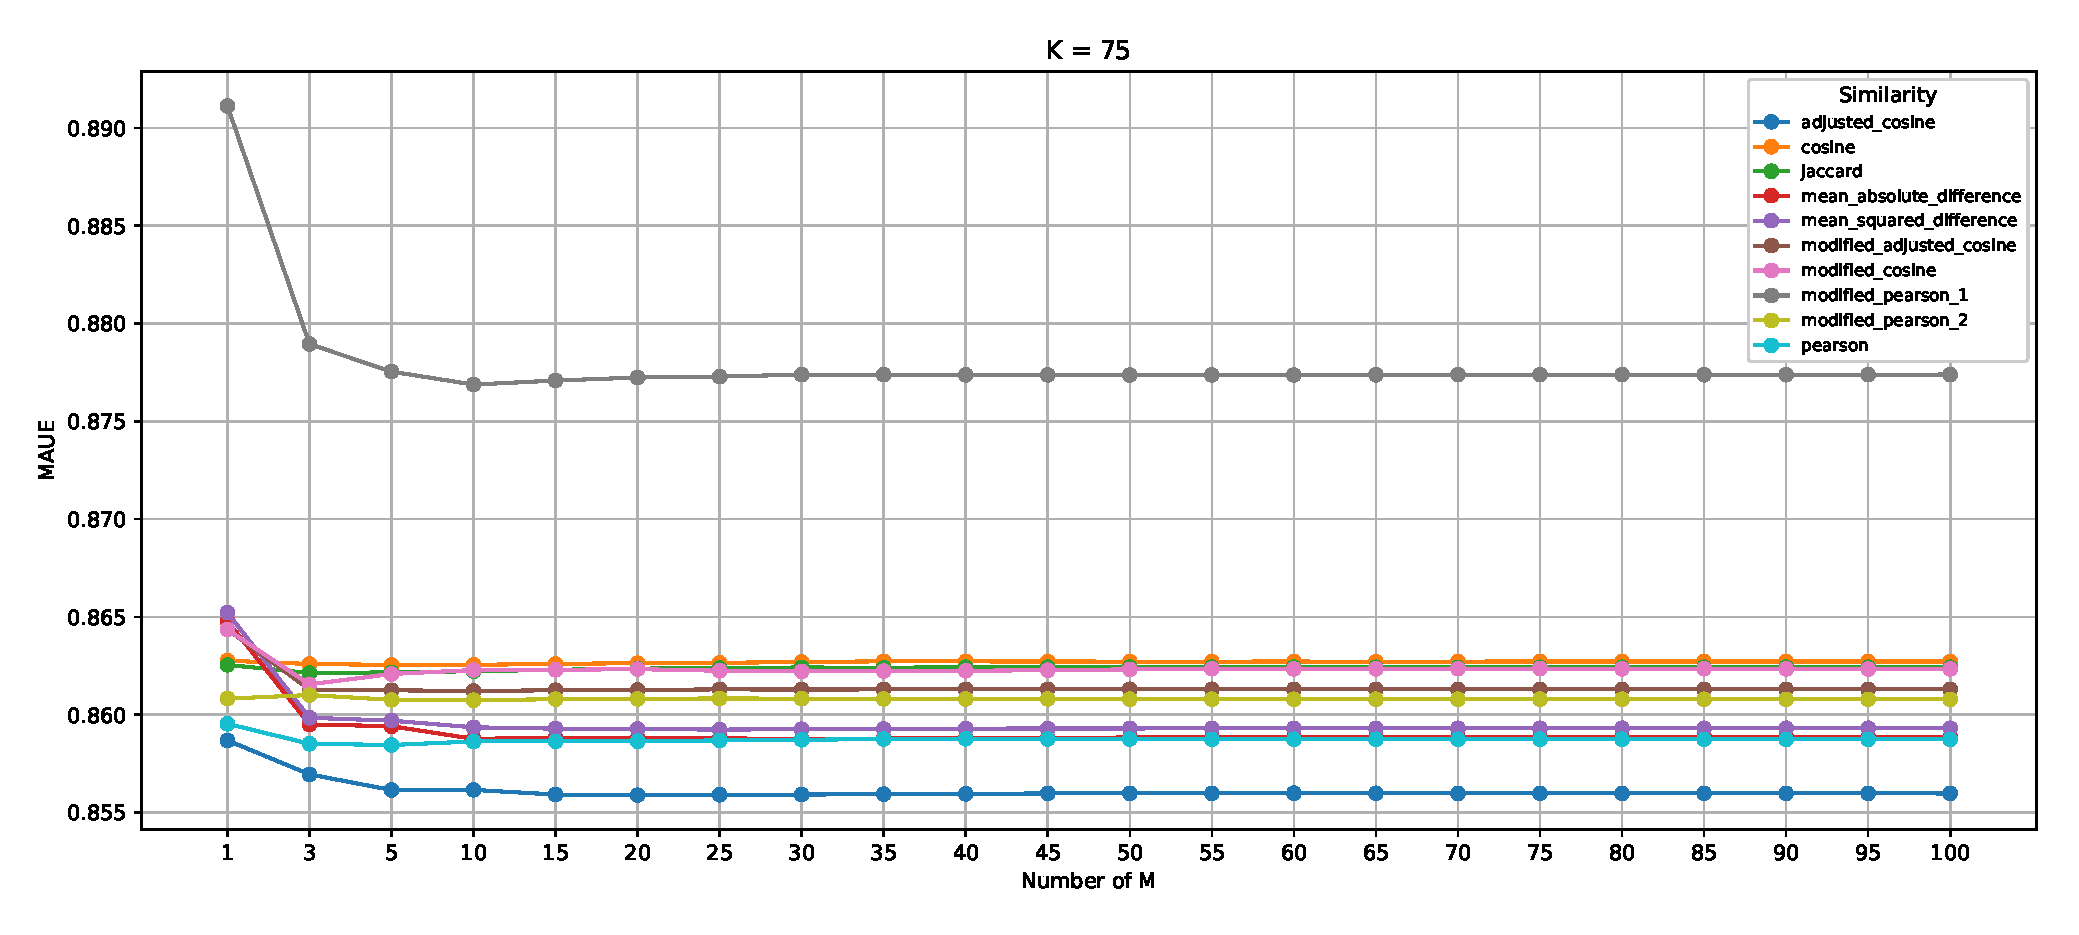
\includegraphics[width=1\textwidth]{chapter_4/evaluation/evaluation_user_maue.eps}
\caption{User-based Recursive-KNN MAUE Best Score}
\label{figure:User_rknn_maue}
\end{figure}

The best Recursive-KNN MAUE score for user-based CF was produced using $\mathcal{K}=75$ and \\$\mathcal{M}=20$.
The exact Recursive-KNN MAUE score is 0.8558869566 and it was calculated based on 34392 rating predictions(\autoref{table:prediction_counters_by_sim})
using the adjusted cosine similarity(\autoref{eq:adjusted_cosine})
out of the 36278 pairs for which KNN was unable to find neighbors(\autoref{table:users_log}).

\subsection{Item-based}
\begin{figure}[H]
\centering
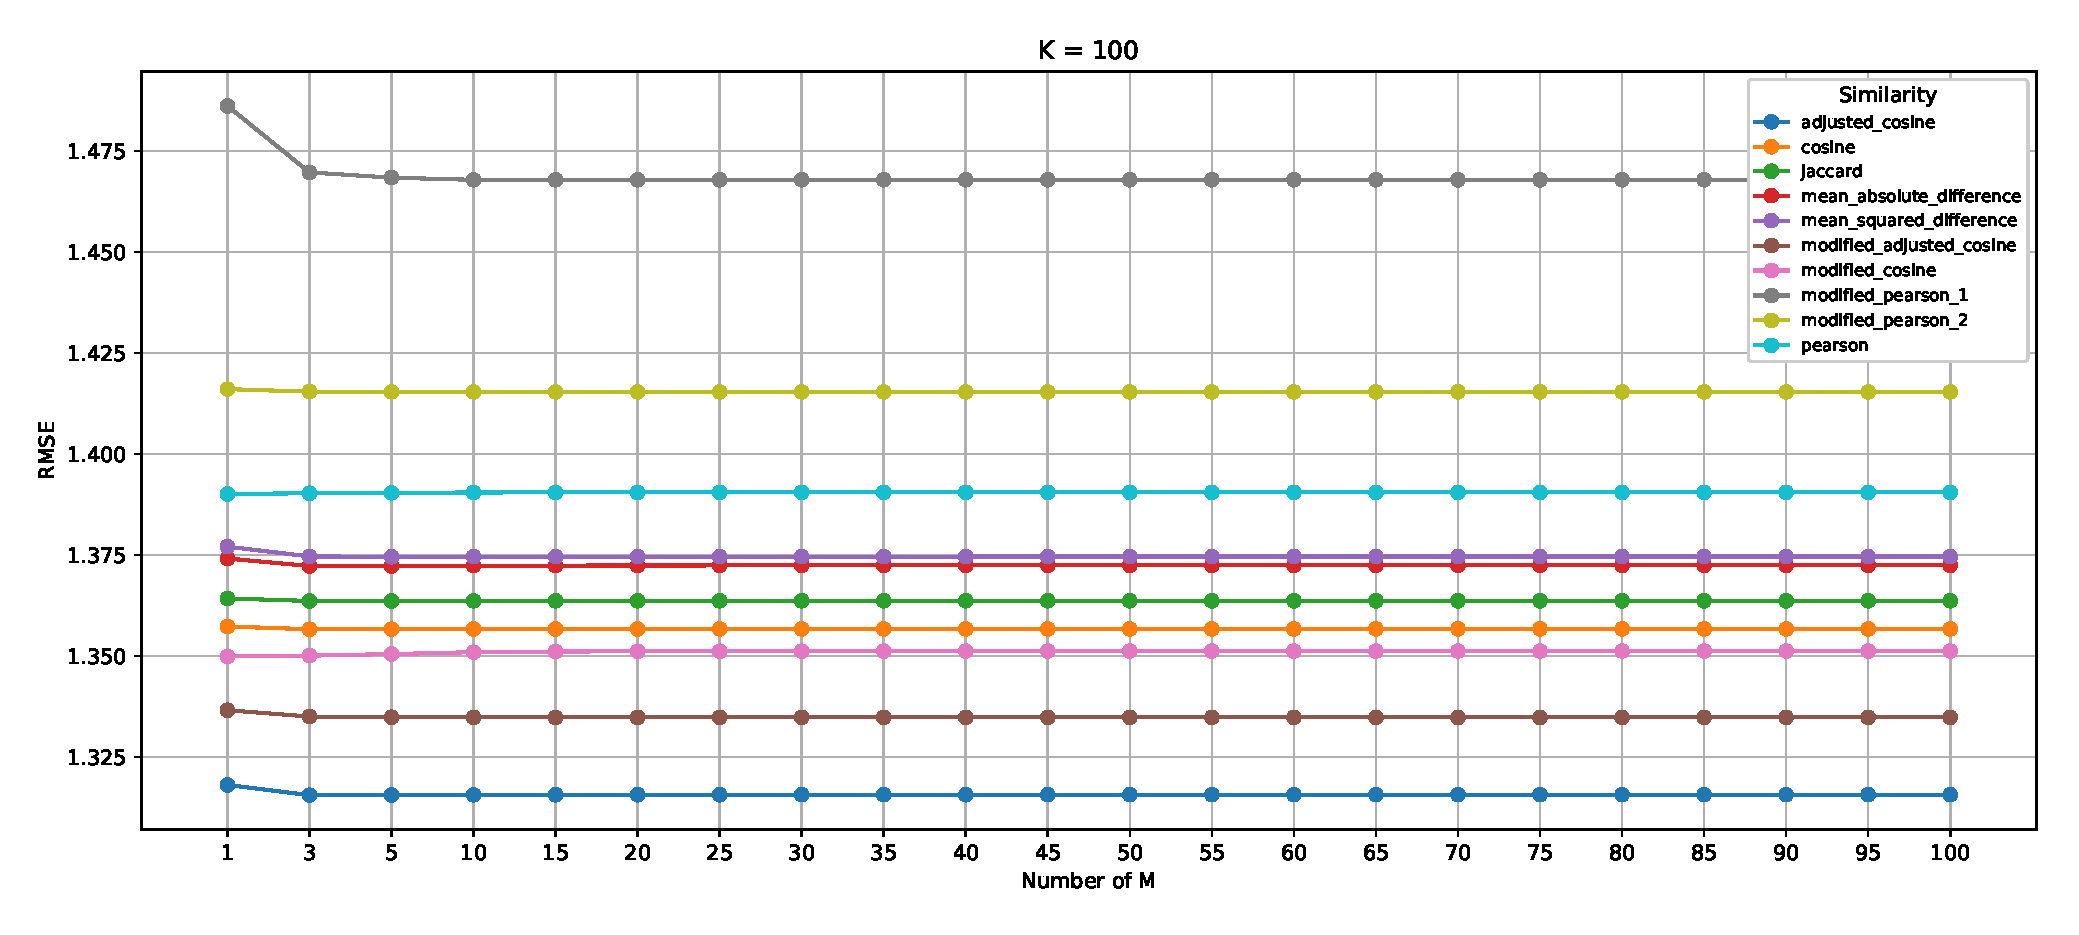
\includegraphics[width=1\textwidth]{chapter_4/evaluation/evaluation_item_rmse.eps}
\caption{Item-based Total RMSE Best Score}
\label{figure:Item_knn_rmse}
\end{figure}

The best RMSE score for item-based CF was produced using $\mathcal{K}=100$ and $\mathcal{M}=3$.
The exact RMSE score is 1.3155259043 and it was calculated based on 123115 rating predictions(\autoref{table:prediction_counters_by_sim})
using the adjusted cosine similarity(\autoref{eq:adjusted_cosine})
for the 144621 ratings in the test set(\autoref{table:epinions_descriptive}).

\begin{figure}[H]
\centering
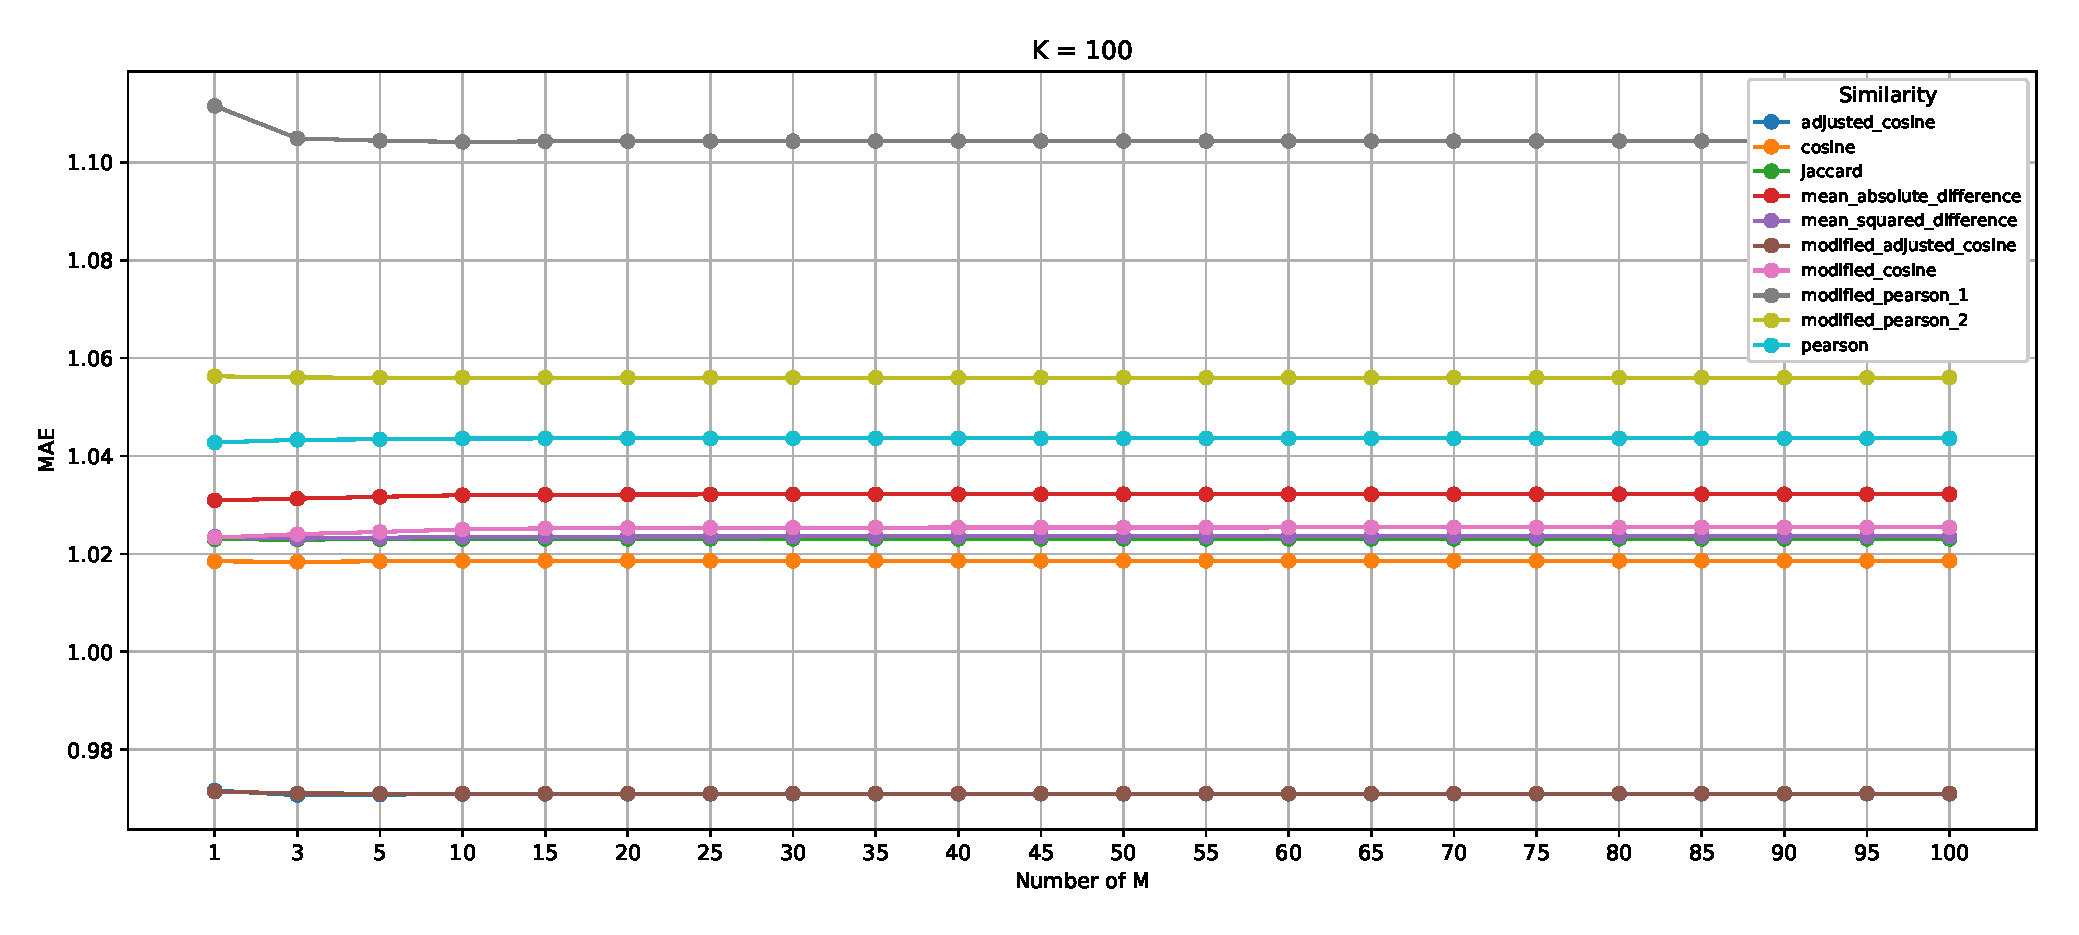
\includegraphics[width=1\textwidth]{chapter_4/evaluation/evaluation_item_mae.eps}
\caption{Item-based Total MAE Best Score}
\label{figure:Item_knn_mae}
\end{figure}

The best MAE score for item-based CF was produced using $\mathcal{K}=100$ and $\mathcal{M}=3$.
The exact MAE score is 0.9707211649 and it was calculated based on 123115 rating predictions(\autoref{table:prediction_counters_by_sim})
using the adjusted cosine similarity(\autoref{eq:adjusted_cosine})
for the 144621 ratings in the test set(\autoref{table:epinions_descriptive}).

\begin{figure}[H]
\centering
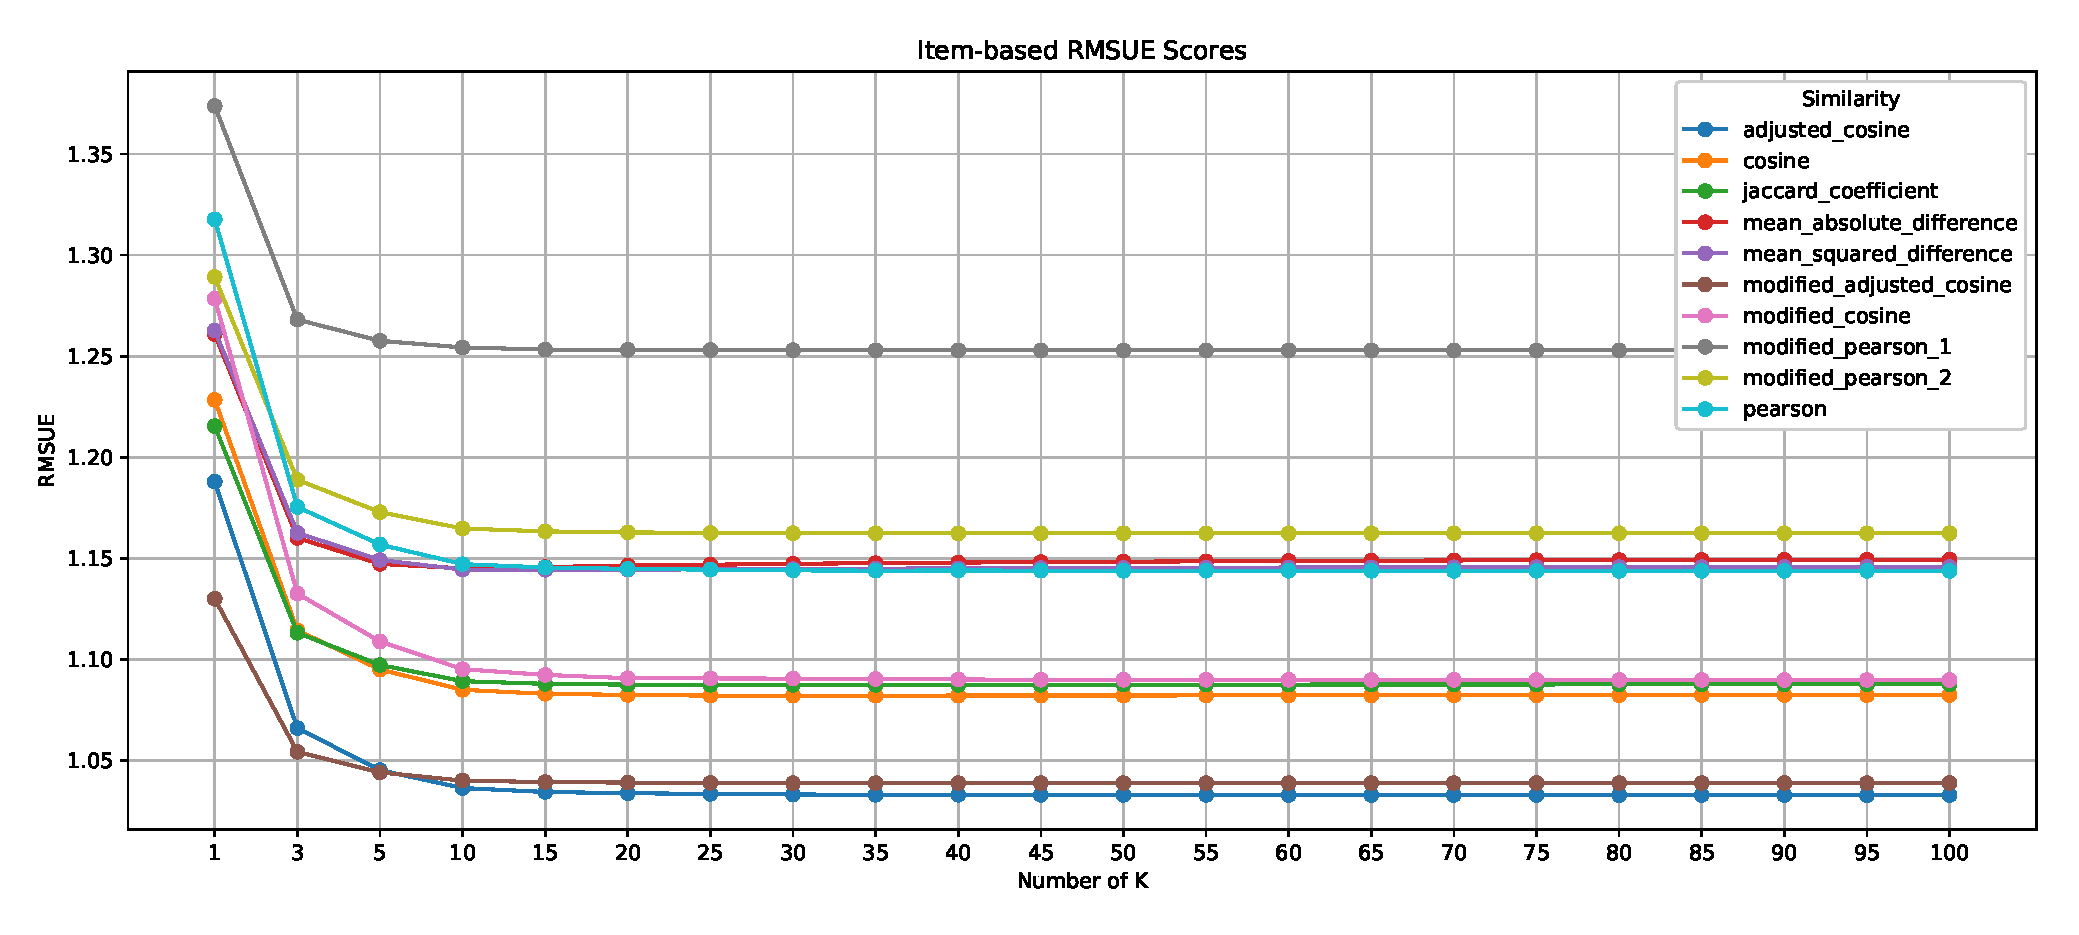
\includegraphics[width=1\textwidth]{chapter_4/knn/Item_RMSUE_KNN.eps}
\caption{Item-based KNN RMSUE Scores}
\label{figure:Item_knn_rmsue}
\end{figure}

The best KNN RMSUE score for item-based CF was produced using $\mathcal{K}=100$.
The exact KNN RMSUE score is 1.0328968801 and it was calculated based on 89800 rating predictions(\autoref{table:prediction_counters_by_sim})
using the adjusted cosine similarity(\autoref{eq:adjusted_cosine})
for the 144621 ratings in the test set(\autoref{table:epinions_descriptive}).

\begin{figure}[H]
\centering
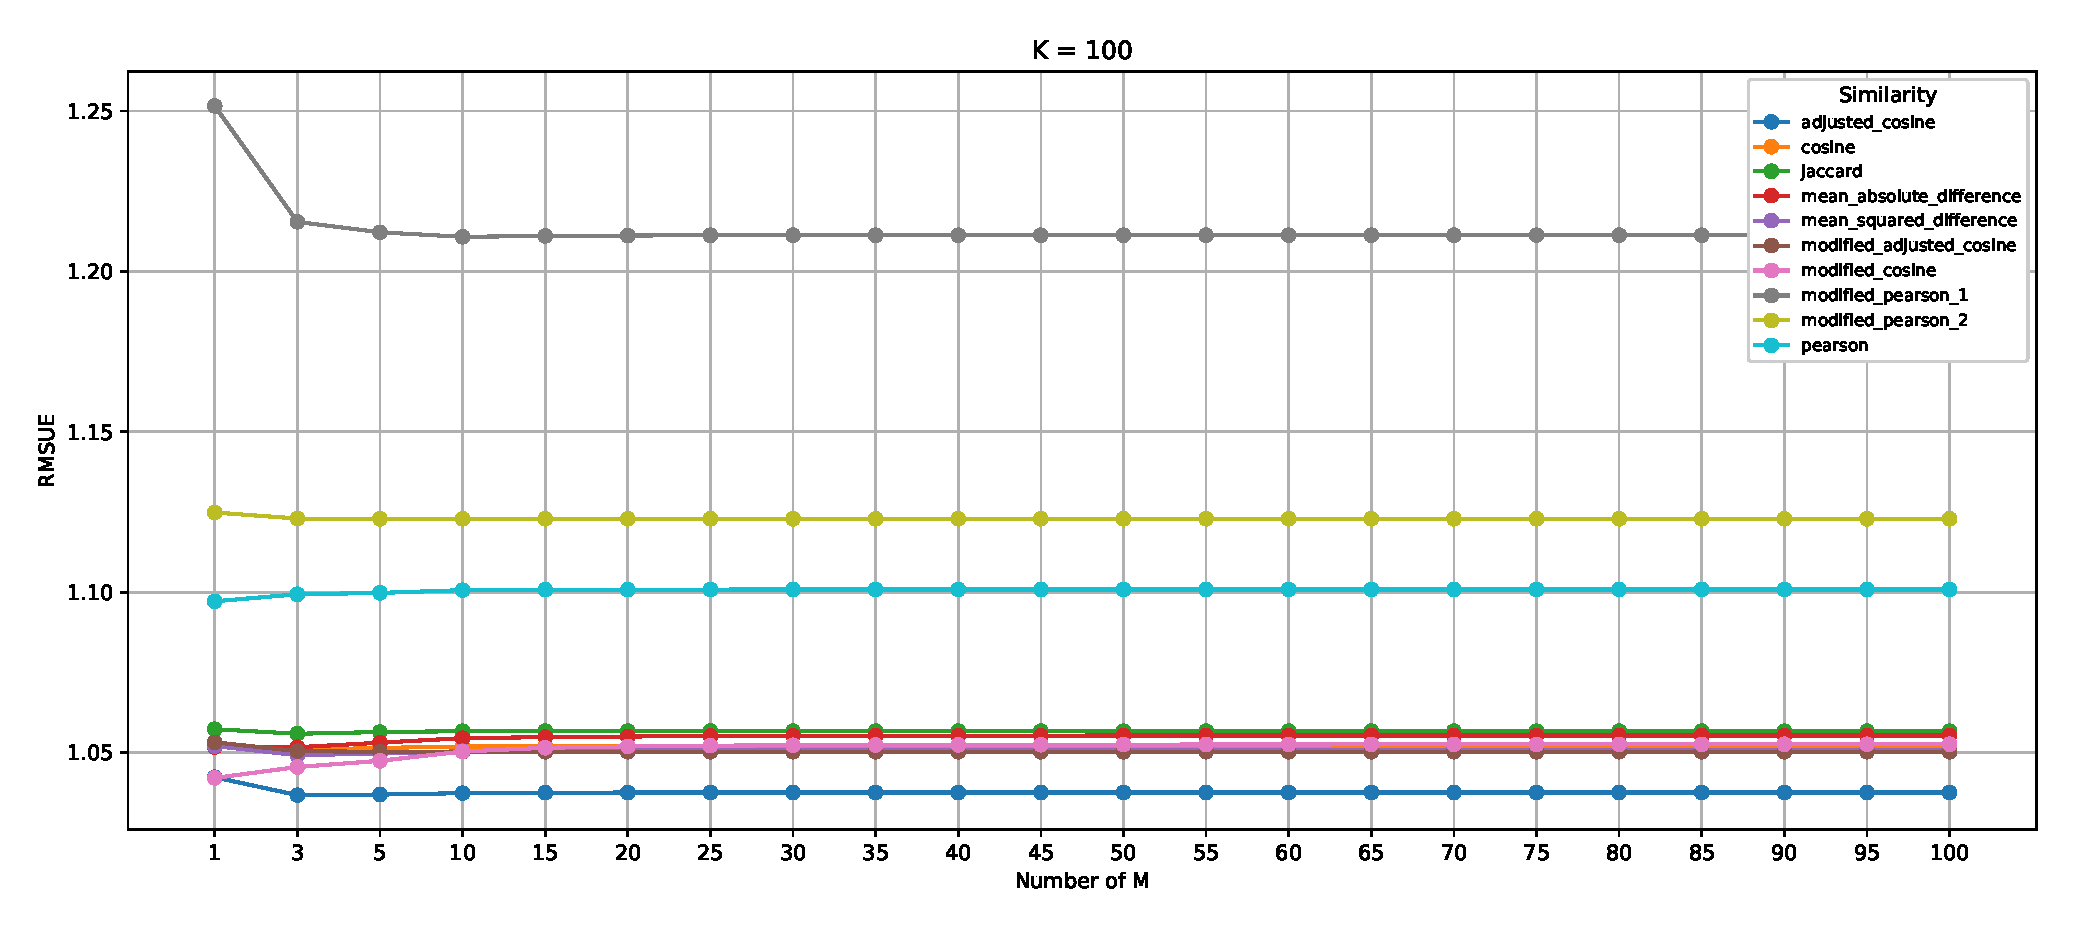
\includegraphics[width=1\textwidth]{chapter_4/evaluation/evaluation_item_rmsue.eps}
\caption{Item-based Recursive-KNN RMSUE Best Score}
\label{figure:Item_rknn_rmsue}
\end{figure}

The best Recursive-KNN RMSUE score for item-based CF was produced using $\mathcal{K}=100$ and $\mathcal{M}=3$.
The exact Recursive-KNN RMSUE score is 1.0367245756 and it was calculated based on 33315 rating predictions(\autoref{table:prediction_counters_by_sim})
using the adjusted cosine similarity(\autoref{eq:adjusted_cosine})
out of the 35280 pairs for which KNN was unable to find neighbors(\autoref{table:items_log}).

\begin{figure}[H]
\centering
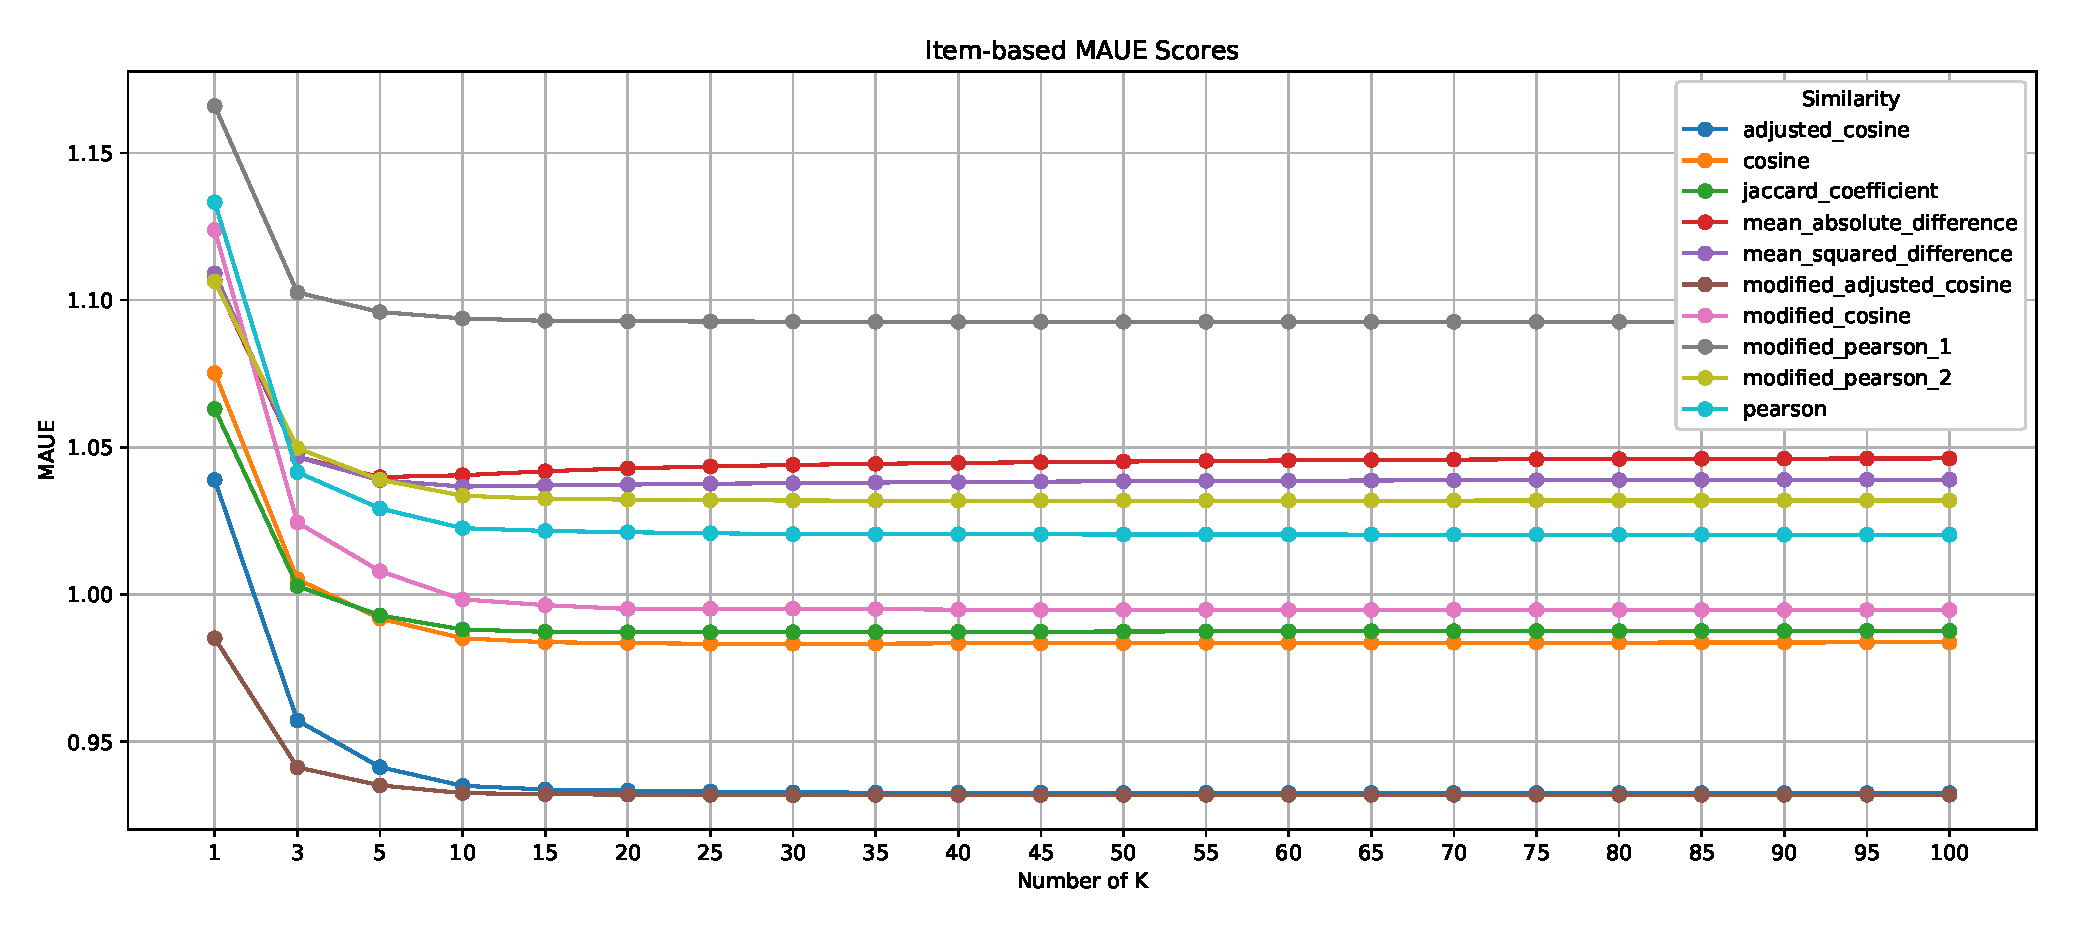
\includegraphics[width=1\textwidth]{chapter_4/knn/Item_MAUE_KNN.eps}
\caption{Item-based KNN MAUE Scores}
\label{figure:Item_knn_maue}
\end{figure}

The best KNN MAUE score for item-based CF was produced using $\mathcal{K}=30$.
The exact KNN MAUE score is 0.9318609947 and it was calculated based on 89800 rating predictions(\autoref{table:prediction_counters_by_sim})
using the modified adjusted cosine similarity(\autoref{eq:modified_adjusted_cosine})
for the 144621 ratings in the test set(\autoref{table:epinions_descriptive}).

\begin{figure}[H]
\centering
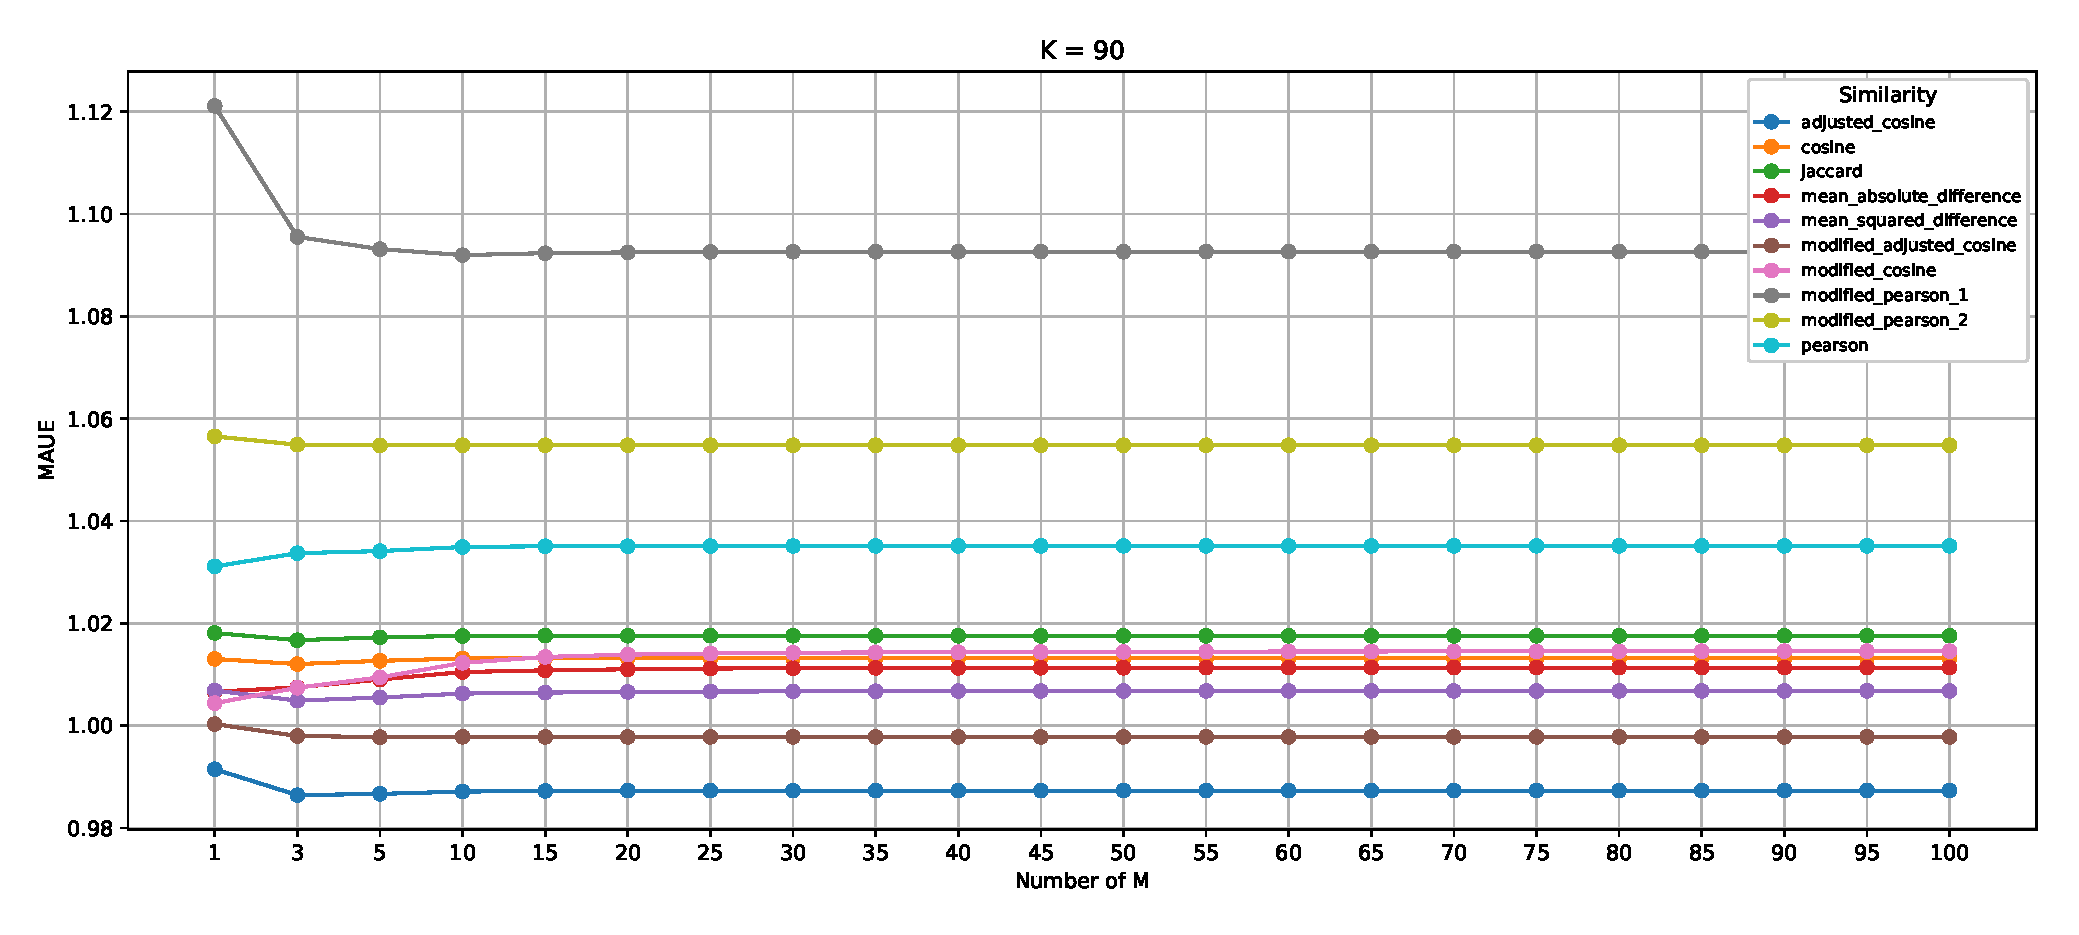
\includegraphics[width=1\textwidth]{chapter_4/evaluation/evaluation_item_maue.eps}
\caption{Item-based KNN MAUE Best Score}
\label{figure:Item_rknn_maue}
\end{figure}

The best Recursive-KNN MAUE score for item-based CF was produced using $\mathcal{K}=90$ and $\mathcal{M}=3$.
The exact Recursive-KNN MAUE score is 0.9864005988 and it was calculated based on 33315 rating predictions(\autoref{table:prediction_counters_by_sim})
using the adjusted cosine similarity(\autoref{eq:adjusted_cosine})
out of the 35280 pairs for which KNN was unable to find neighbors(\autoref{table:items_log}).

\subsection{Benchmarks}
\begin{table}[H]
\centering
\caption{Rating Predicted with KNN and Recursive-KNN}
\label{table:prediction_counters_by_sim}
\begin{tabular}{ccc|ccc|c}
\multicolumn{3}{c|}{\textbf{USERS}}            & \multicolumn{3}{c|}{\textbf{ITEMS}}            &                          \\ \cline{1-6}
\textbf{KNN} & \textbf{R-KNN} & \textbf{TOTAL} & \textbf{KNN} & \textbf{R-KNN} & \textbf{TOTAL} & \textbf{SIMILARITY}      \\ \hline
88379        & 34392          & 122771         & 89800        & 33315          & 123115         & Adjusted Cosine          \\
\textbf{100311}       & 24122          & \textbf{124433}         & \textbf{100311}       & 24122          & \textbf{124433}         & Cosine                   \\
\textbf{100311}       & 24122          & \textbf{124433}         & \textbf{100311}       & 24122          & \textbf{124433}         & Jaccard                  \\
93924        & 29747          & 123671         & 94528        & 29203          & 123731         & MAD                      \\
93924        & 29747          & 123671         & 94528        & 29203          & 123731         & MSD                      \\
88379        & 34392          & 122771         & 89800        & 33315          & 123115         & Modified Adjusted Cosine \\
\textbf{100311}       & 24122          & \textbf{124433}         & \textbf{100311}       & 24122          & \textbf{124433}         & Modified Cosine          \\
59017        & \textbf{40470}          & 99487          & 54644        & \textbf{34096}          & 88740          & Modified Pearson 1       \\
89936        & 28183          & 118119         & 84511        & 24357          & 108868         & Modified Pearson 2       \\
89936        & 28183          & 118119         & 84511        & 24357          & 108868         & Pearson
\end{tabular}
\end{table}

Cosine, Jaccard and Modified Cosine were able to produce the most rating predictions, 124433 in total,
both for user-based and item-based. Modified Pearson 1 was the one with the least similarities
(\autoref{table:modified_pearson_1_descriptive}) and therefore the one with the least rating
predictions, even though, it managed to predict a total of 99487 ratings user-based
and 88740 item-based. The outcome however was very poor for this similarity formula for any
evaluation metric. The average boost in rating predictions using the Recursive-KNN method was
about 25\% for user-based CF and 24\% for item-based CF.
\newpage
The two tables below are the logs produced for user-based(\autoref{table:users_log})
and item-based(\autoref{table:items_log}) KNN and Recursive-KNN algorithms.
The first three columns refer to the KNN algorithm and present the number of pairs that KNN
algorithm was unable to predict. The first column indicates the number of pairs
(user, item) for which relevant nearest neighbors did not exist. The second column
indicates the number of pairs that either the item in user-based or user in
item-based did not exist in the train set. The third column indicates the number
of pairs that either the user in user-based or item in
item-based did not exist in the train set and therefore KNN could not find similarities.
The test was for 22 different values of $\mathcal{K}$. The total compute time for each similarity
metric for all $\mathcal{K}$'s is indicated in the fourth column.
The next two columns refer to Recursive-KNN algorithm. The fifth column indicates
the number of pairs that could not be predicted due to no further neighbors
after the completion of the Recursive-KNN algorithm.
The sixth column is the time the Recursive-KNN took for completing all the available combinations
484 in count between $\mathcal{K}$'s and $\mathcal{M}$'s (i.e. ($\mathcal{M}$=1, $\mathcal{K}$=1),
($\mathcal{M}$=1, $\mathcal{K}$=3), ($\mathcal{M}$=3, $\mathcal{K}$=1) e.t.c.).

The computations were run on a cloud computing platform.
The specifications of the machine were the following:
\begin{itemize}
	\item[] \textbf{OS:} Ubuntu Server 16.04.3
	\item[] \textbf{CPU:} Intel Xeon E5-2697A v4 @ 2.60GHz
	\item[] \textbf{RAM:} 3GB DDR4 + 1GB SWAP
\end{itemize}

\begin{table}[H]
\centering
\caption{User-based KNN and Recursive-KNN Log}
\label{table:users_log}
\begin{tabular}{|c|c|c|c|c|c|c|}
\cline{1-6}
\multicolumn{4}{|c|}{\textbf{KNN}}                                               & \multicolumn{2}{c|}{\textbf{Recursive-KNN}} & \multicolumn{1}{l}{}                          \\ \hline
\textbf{No NN} & \textbf{Not in Train} & \textbf{No Similarity} & \textbf{Time} & \textbf{R-No NN} & \textbf{R-Time}		& \multicolumn{1}{c|}{\textbf{Similarity}}      \\ \hline
36278          & 18939                 & 1025                  & 0:3:58        & 1886             & 4:3:9           		& \multicolumn{1}{c|}{adjusted cosine}          \\ \hline
25061          & 18939                 & 310                   & 0:5:17        & 939              & 4:1:57          		& \multicolumn{1}{c|}{cosine}                   \\ \hline
25061          & 18939                 & 310                   & 0:3:41        & 939              & 2:57:58         		& \multicolumn{1}{c|}{jaccard}                  \\ \hline
31200          & 18939                 & 558                   & 0:4:16        & 1453             & 3:2:29          		& \multicolumn{1}{c|}{mad}                      \\ \hline
31200          & 18939                 & 558                   & 0:4:9         & 1453             & 3:9:12          		& \multicolumn{1}{c|}{msd}                      \\ \hline
36278          & 18939                 & 1025                  & 0:4:13        & 1886             & 4:3:56          		& \multicolumn{1}{c|}{modified adjusted cosine} \\ \hline
25061          & 18939                 & 310                   & 0:4:31        & 939              & 2:42:42         		& \multicolumn{1}{c|}{modified cosine}          \\ \hline
48886          & 18939                 & 17779                 & 0:3:8         & 8416             & 1:33:26         		& \multicolumn{1}{c|}{modified pearson 1}       \\ \hline
29450          & 18939                 & 6296                  & 0:3:18        & 1267             & 3:4:17          		& \multicolumn{1}{c|}{modified pearson 2}       \\ \hline
29450          & 18939                 & 6296                  & 0:3:8         & 1267             & 2:48:48         		& \multicolumn{1}{c|}{pearson}                  \\ \hline
\end{tabular}
\end{table}

\begin{table}[H]
\centering
\caption{Item-based KNN and Recursive-KNN Log}
\label{table:items_log}
\begin{tabular}{|c|c|c|c|c|c|c}
\cline{1-6}
\multicolumn{4}{|c|}{\textbf{KNN}}                                               & \multicolumn{2}{c|}{\textbf{Recursive-KNN}} & \multicolumn{1}{l}{}                          \\ \hline
\textbf{No NN} & \textbf{Not in  Train} & \textbf{No Similarity} & \textbf{Time} & \textbf{R-No NN}      & \textbf{R-Time}     & \multicolumn{1}{c|}{\textbf{Similarity}}      \\ \hline
35280          & 0                      & 19541                  & 0:3:2         & 1965                  & 2:18:35             & \multicolumn{1}{c|}{adjusted cosine}          \\ \hline
25188          & 0                      & 19122                  & 0:3:43        & 1066                  & 2:26:56             & \multicolumn{1}{c|}{cosine}                   \\ \hline
25188          & 0                      & 19122                  & 0:3:37        & 1066                  & 2:12:56             & \multicolumn{1}{c|}{jaccard}                  \\ \hline
30827          & 0                      & 19266                  & 0:3:22        & 1624                  & 1:54:18             & \multicolumn{1}{c|}{mad}                      \\ \hline
30827          & 0                      & 19266                  & 0:3:28        & 1624                  & 1:58:50             & \multicolumn{1}{c|}{msd}                      \\ \hline
35280          & 0                      & 19541                  & 0:3:10        & 1965                  & 2:32:4              & \multicolumn{1}{c|}{modified adjusted cosine} \\ \hline
25188          & 0                      & 19122                  & 0:3:37        & 1066                  & 2:11:18             & \multicolumn{1}{c|}{modified cosine}          \\ \hline
41037          & 0                      & 48940                  & 0:2:14        & 6941                  & 0:39:1              & \multicolumn{1}{c|}{modified pearson 1}       \\ \hline
25332          & 0                      & 34778                  & 0:2:58        & 975                   & 1:49:35             & \multicolumn{1}{c|}{modified pearson 2}       \\ \hline
25332          & 0                      & 34778                  & 0:2:52        & 975                   & 1:46:24             & \multicolumn{1}{c|}{pearson}                  \\ \hline
\end{tabular}
\end{table}


\chapter{Conclusion and future work}
\label{chap:5}
% !TeX root = ../main.tex

\section{Conclusion}
In this thesis a novel approach was proposed in the context of neighborhood-based
collaborative filtering. This approach managed to overcome the limitation
of sparsity that prevented the rating prediction of many user-item pairs.
In fact, it accomplished an average of 25\% increase in the amount of ratings that could be
predicted. The results showed that for Recursive-KNN to be efficient,
the value of $\mathcal{K}$ that indicates the users that will be used to make the final prediction
for the user-item pair should be a large number. Another indication we got from the
results of the Recursive-KNN is that the $\mathcal{M}$ parameter should be low, as
$\mathcal{M}=3$ yielded the best score in the most cases. The user-based approach was more
efficient with this particular data set. Cosine similarity, Modified cosine
similarity and Jaccard coefficient created the most efficient similarities for
the trained model.
\section{Future Work}
To consider Recursive-KNN as a good option for rating predictions, more tests
should be done in order to optimize its accuracy.
\begin{itemize}
    \item[] \textbf{Similarity information:} For these experiments only the
    positive similarities were kept in order to provide predictions. As a
    further study we will properly use all the available information given
    by each similarity, including the negative similarities, and how to
    properly utilize them.
    \item[] \textbf{Similarity re-computation:} After the computations of the KNN algorithm
    we can try to include the predictions in the ratings matrix in order to re-calculate the similarities
    between users or items and test how much more predictions we can further
    find and how much this will affect the accuracy.
    \item[] \textbf{Prediction formula:} For these experiments we only used
    the weighted sum formula to calculate the predictions. We should see
    if we can get any better results by using different formulas.
\end{itemize}


\bibliography{references}

\appendix
\chapter{Source Code}
\label{chap:appendix_src}
% !TeX root = ../main.tex

The source code for this thesis can be found at
\href{https://github.com/tseste/Recursive-K-Nearest-Neighbors}{\color{blue}Github}


\chapter{Experimental Results}
\label{chap:appendix_results}
% !TeX root = ../main.tex

\section{KNN Scores}

\subsection{MAE}

\begin{figure}[H]
\centering
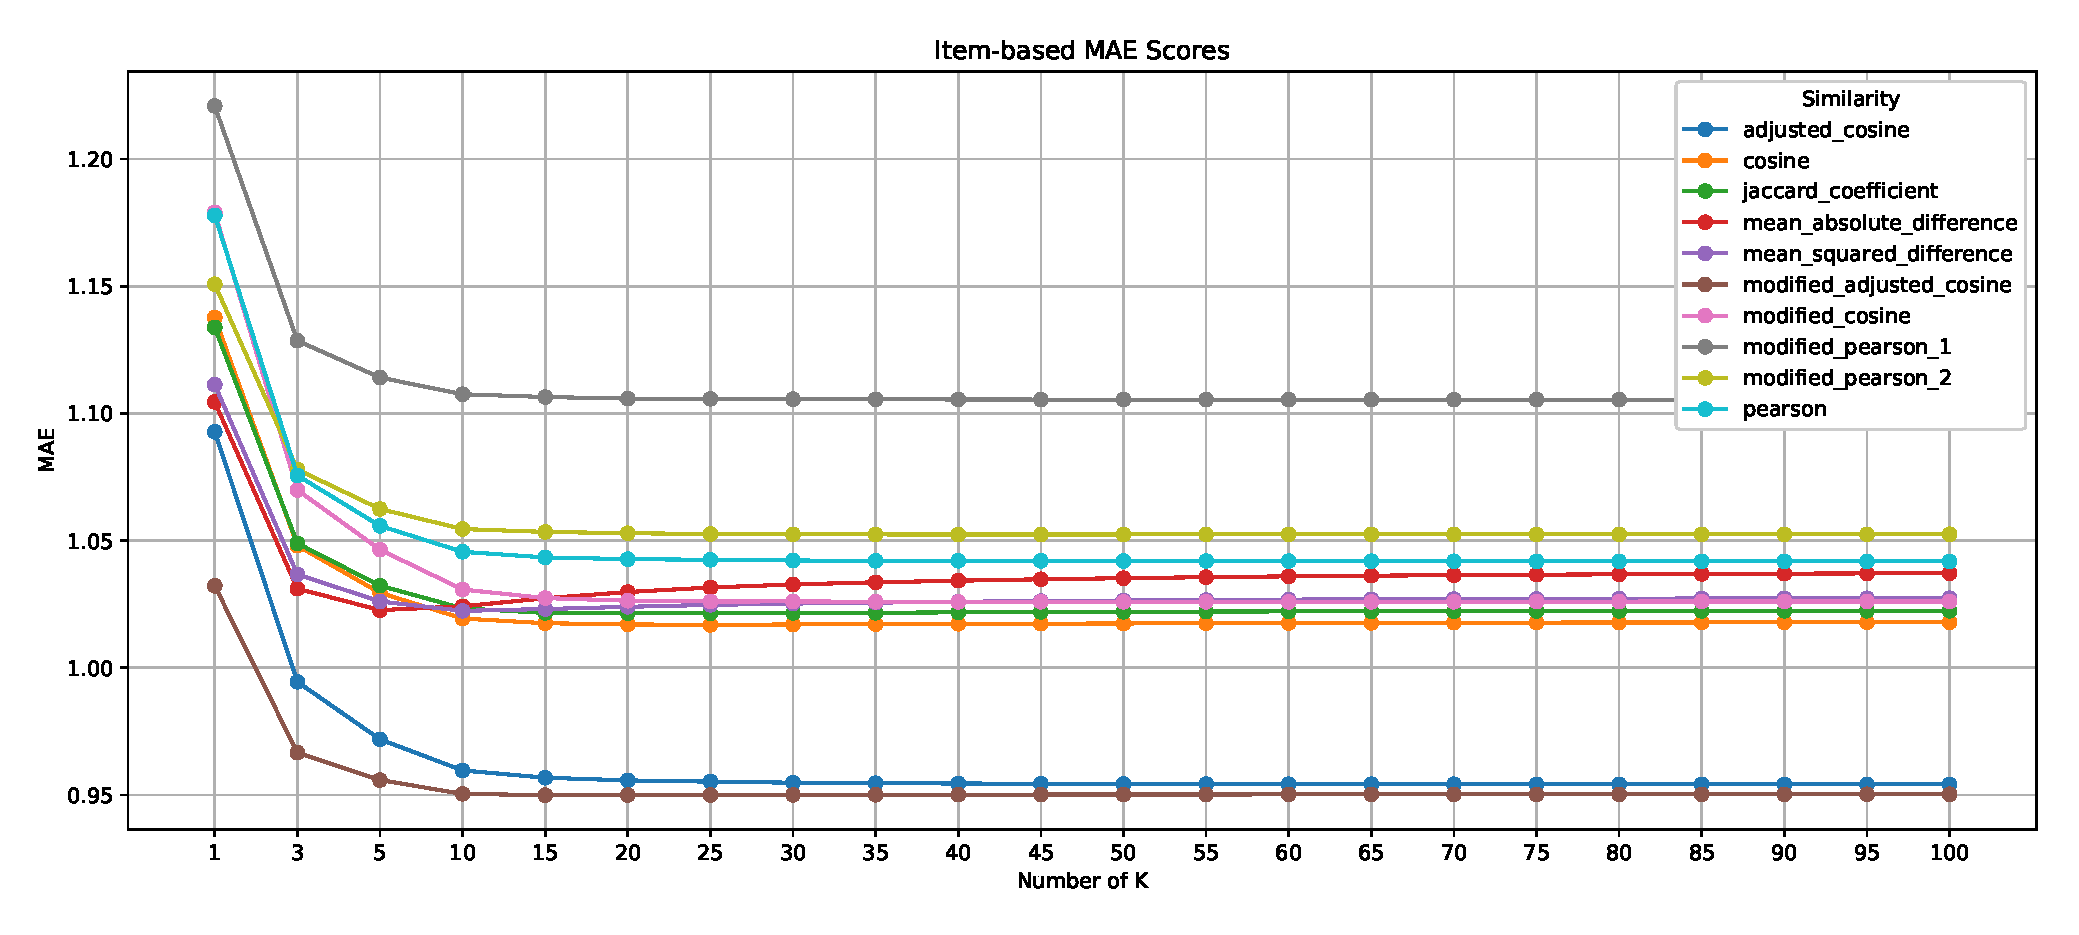
\includegraphics[width=1\textwidth]{chapter_4/knn/Item_MAE_KNN.eps}
\caption{Item-based KNN MAE scores}
\end{figure}

\begin{figure}[H]
\centering
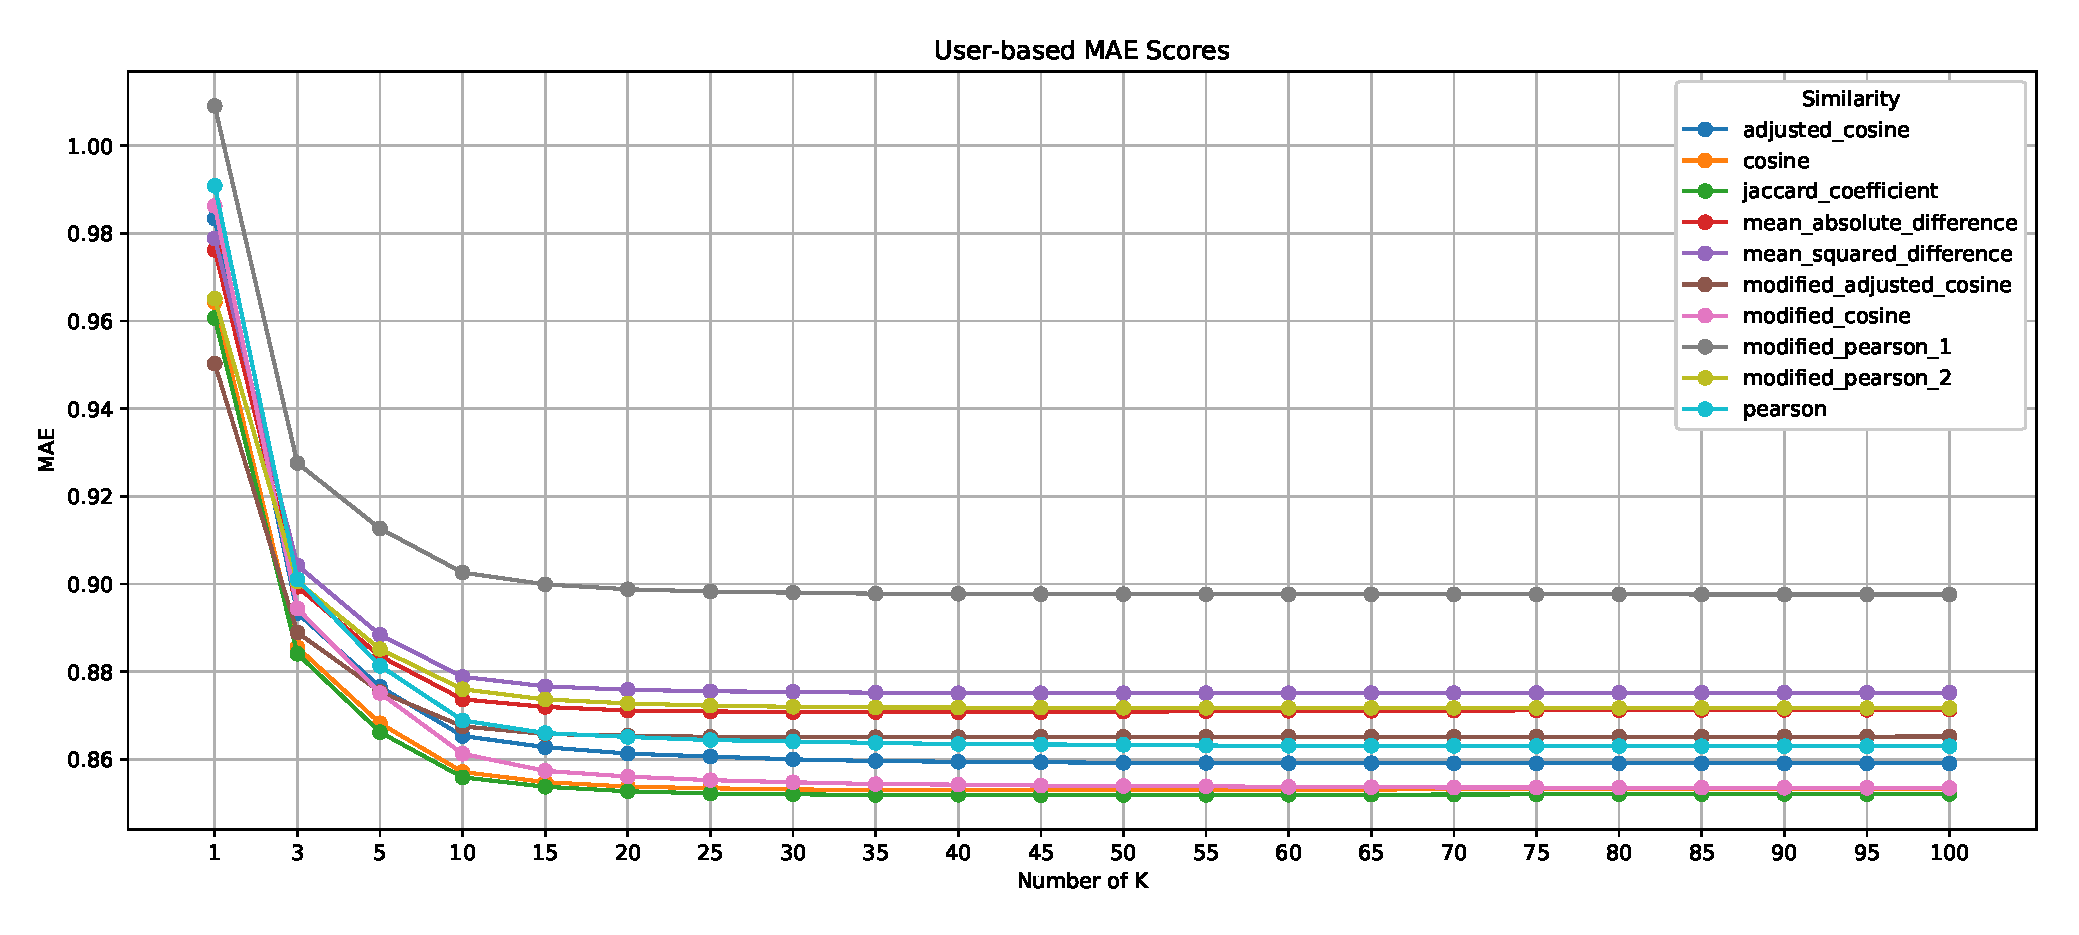
\includegraphics[width=1\textwidth]{chapter_4/knn/User_MAE_KNN.eps}
\caption{User-based KNN MAE scores}
\end{figure}

\subsection{RMSE}

\begin{figure}[H]
\centering
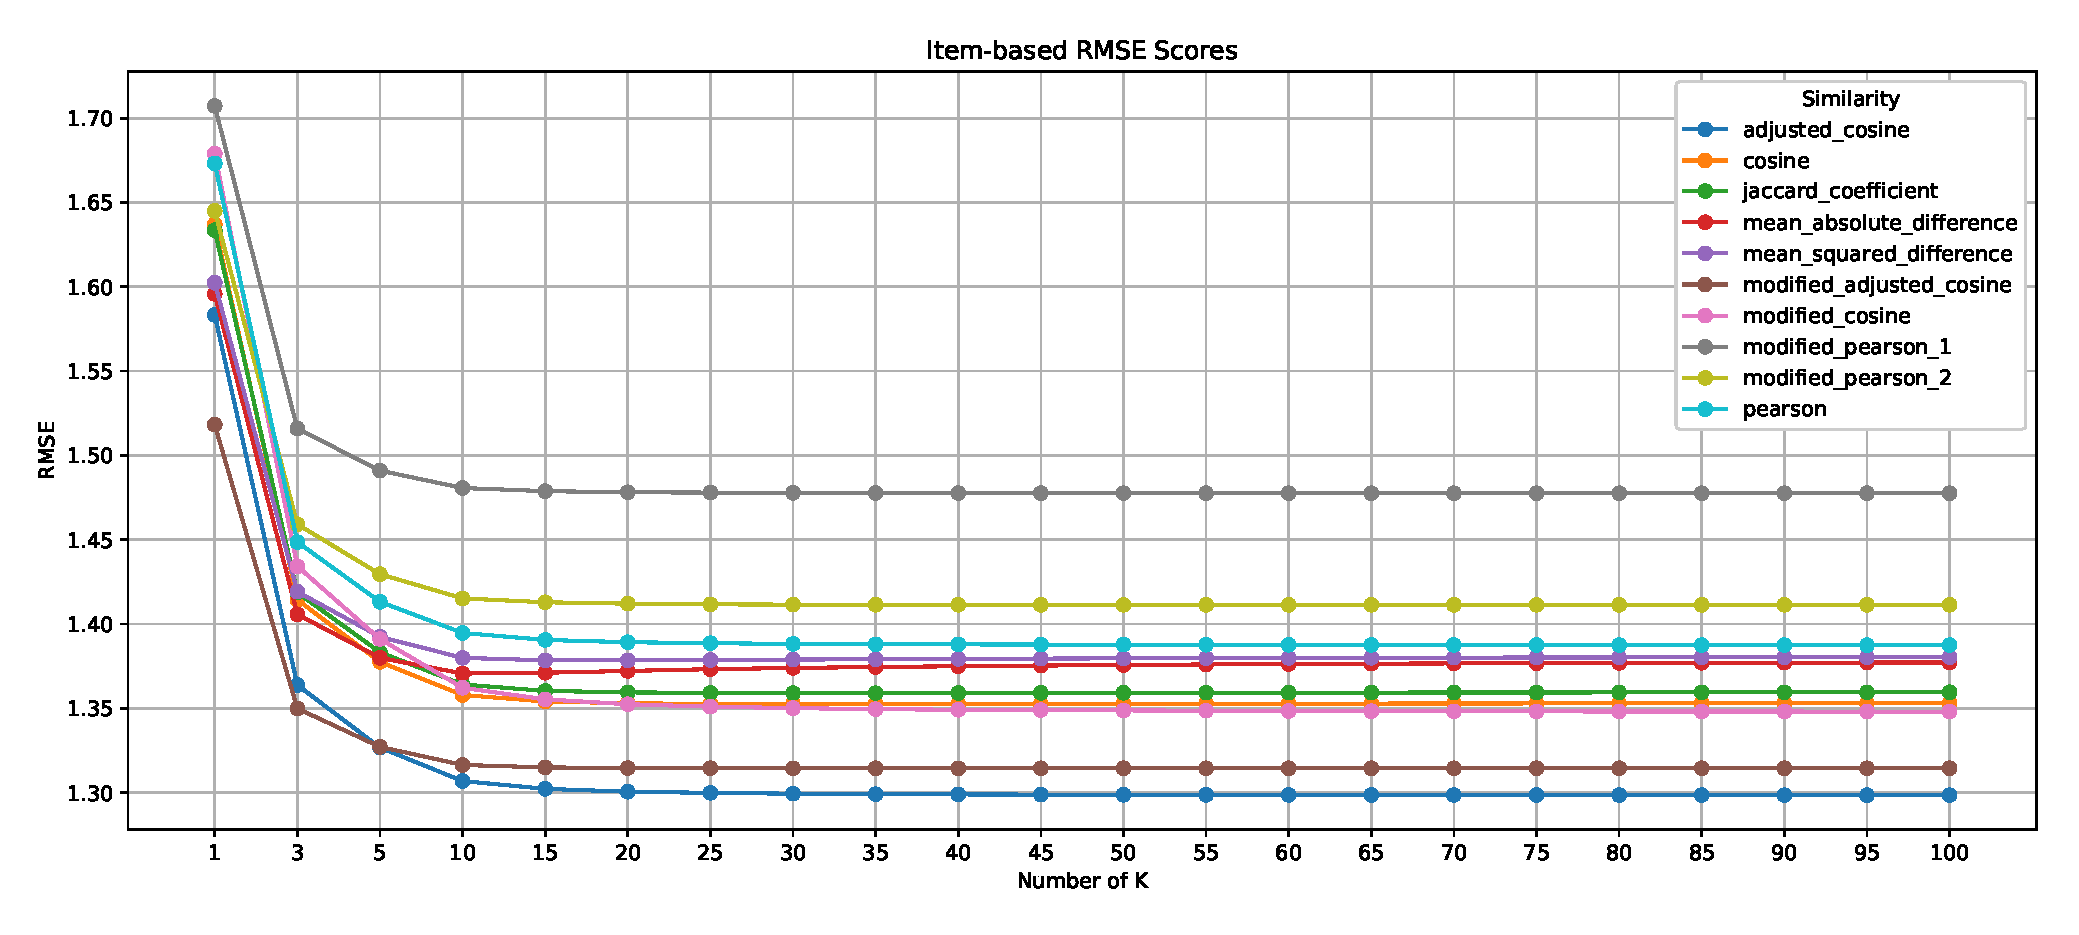
\includegraphics[width=1\textwidth]{chapter_4/knn/Item_RMSE_KNN.eps}
\caption{Item-based KNN RMSE scores}
\end{figure}

\begin{figure}[H]
\centering
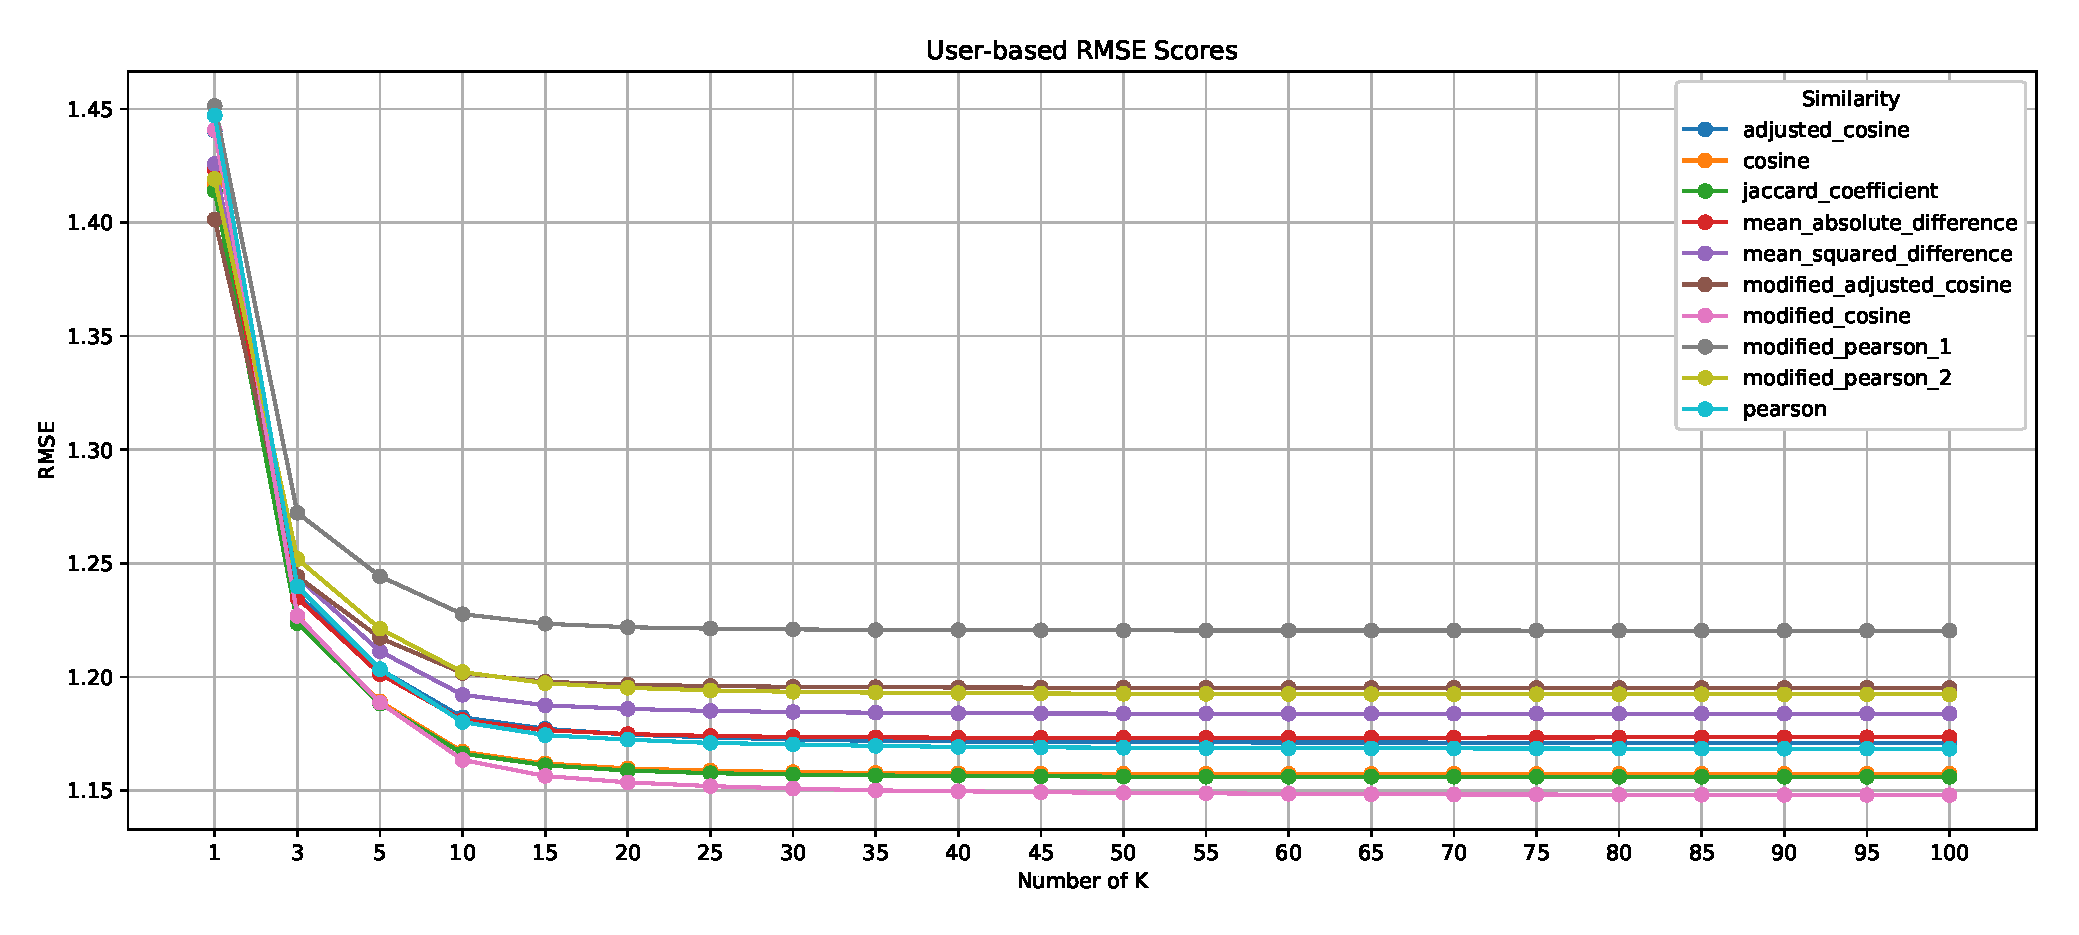
\includegraphics[width=1\textwidth]{chapter_4/knn/User_RMSE_KNN.eps}
\caption{User-based KNN RMSE scores}
\end{figure}

\subsection{MAUE}

\begin{figure}[H]
\centering
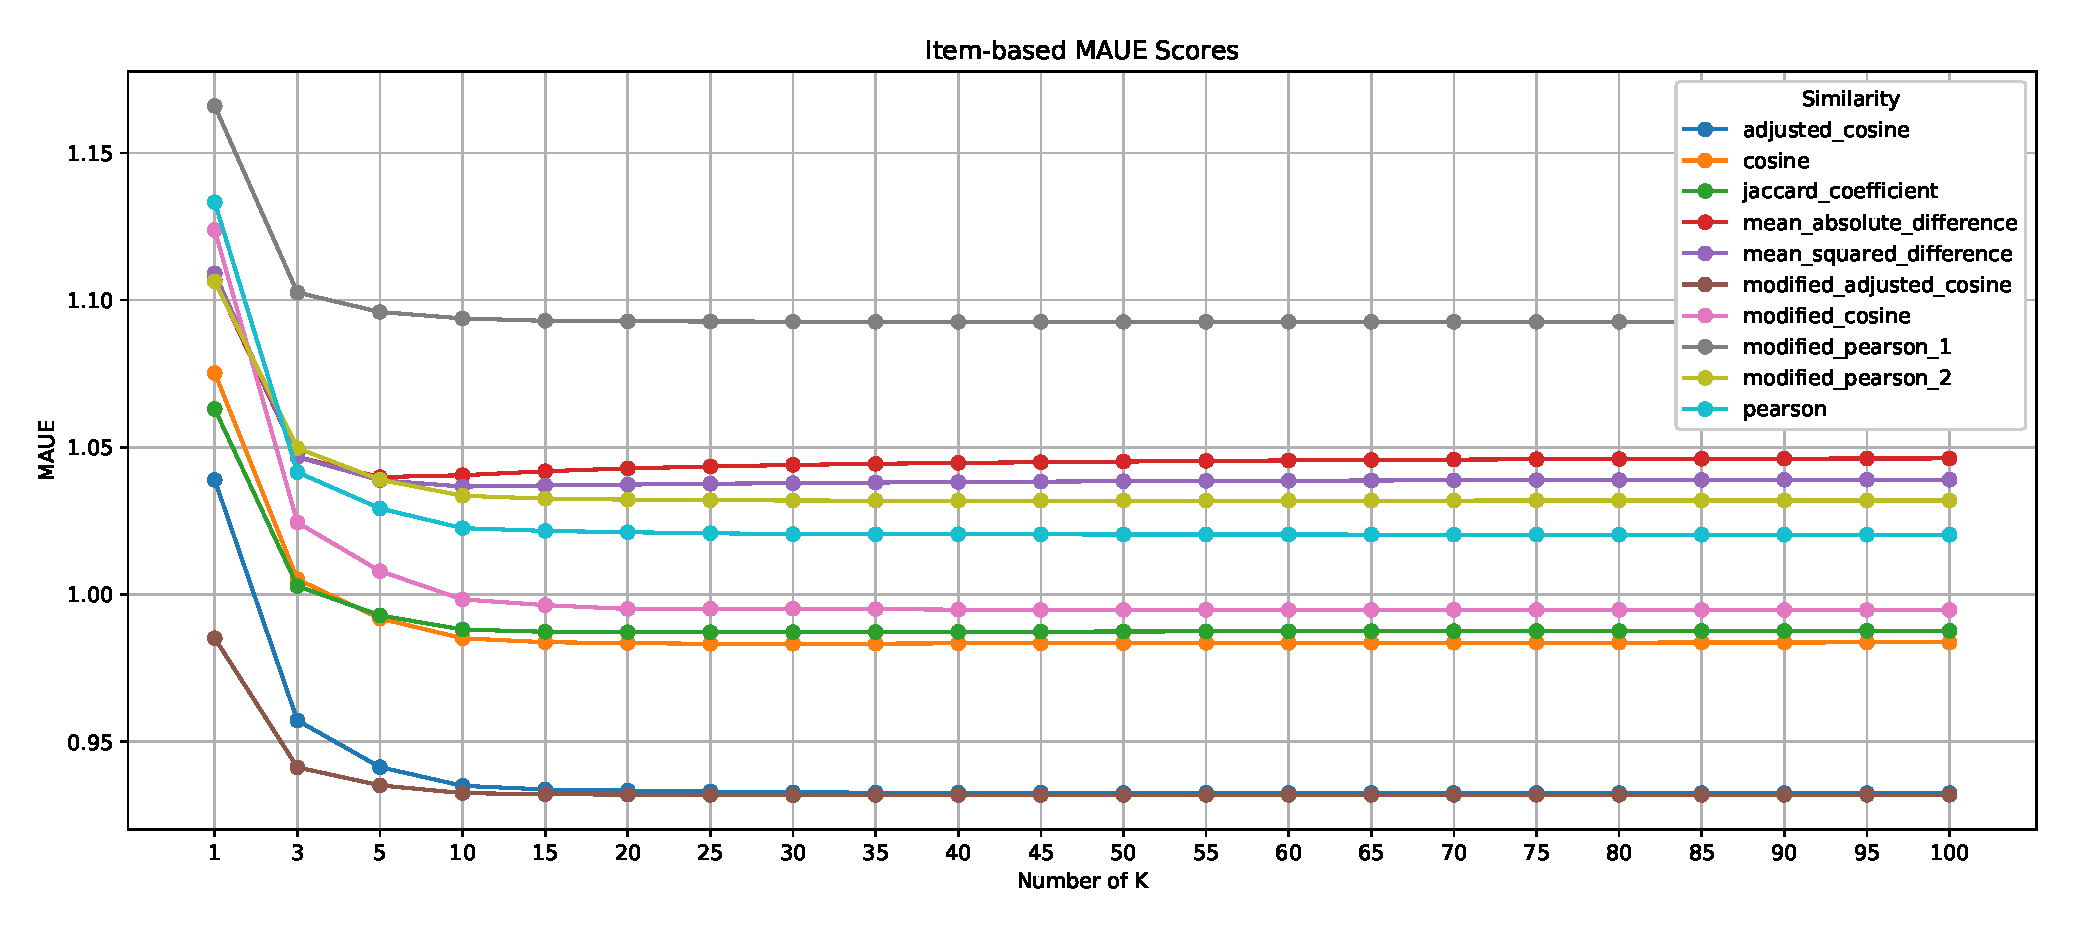
\includegraphics[width=1\textwidth]{chapter_4/knn/Item_MAUE_KNN.eps}
\caption{Item-based KNN MAUE scores}
\end{figure}

\begin{figure}[H]
\centering
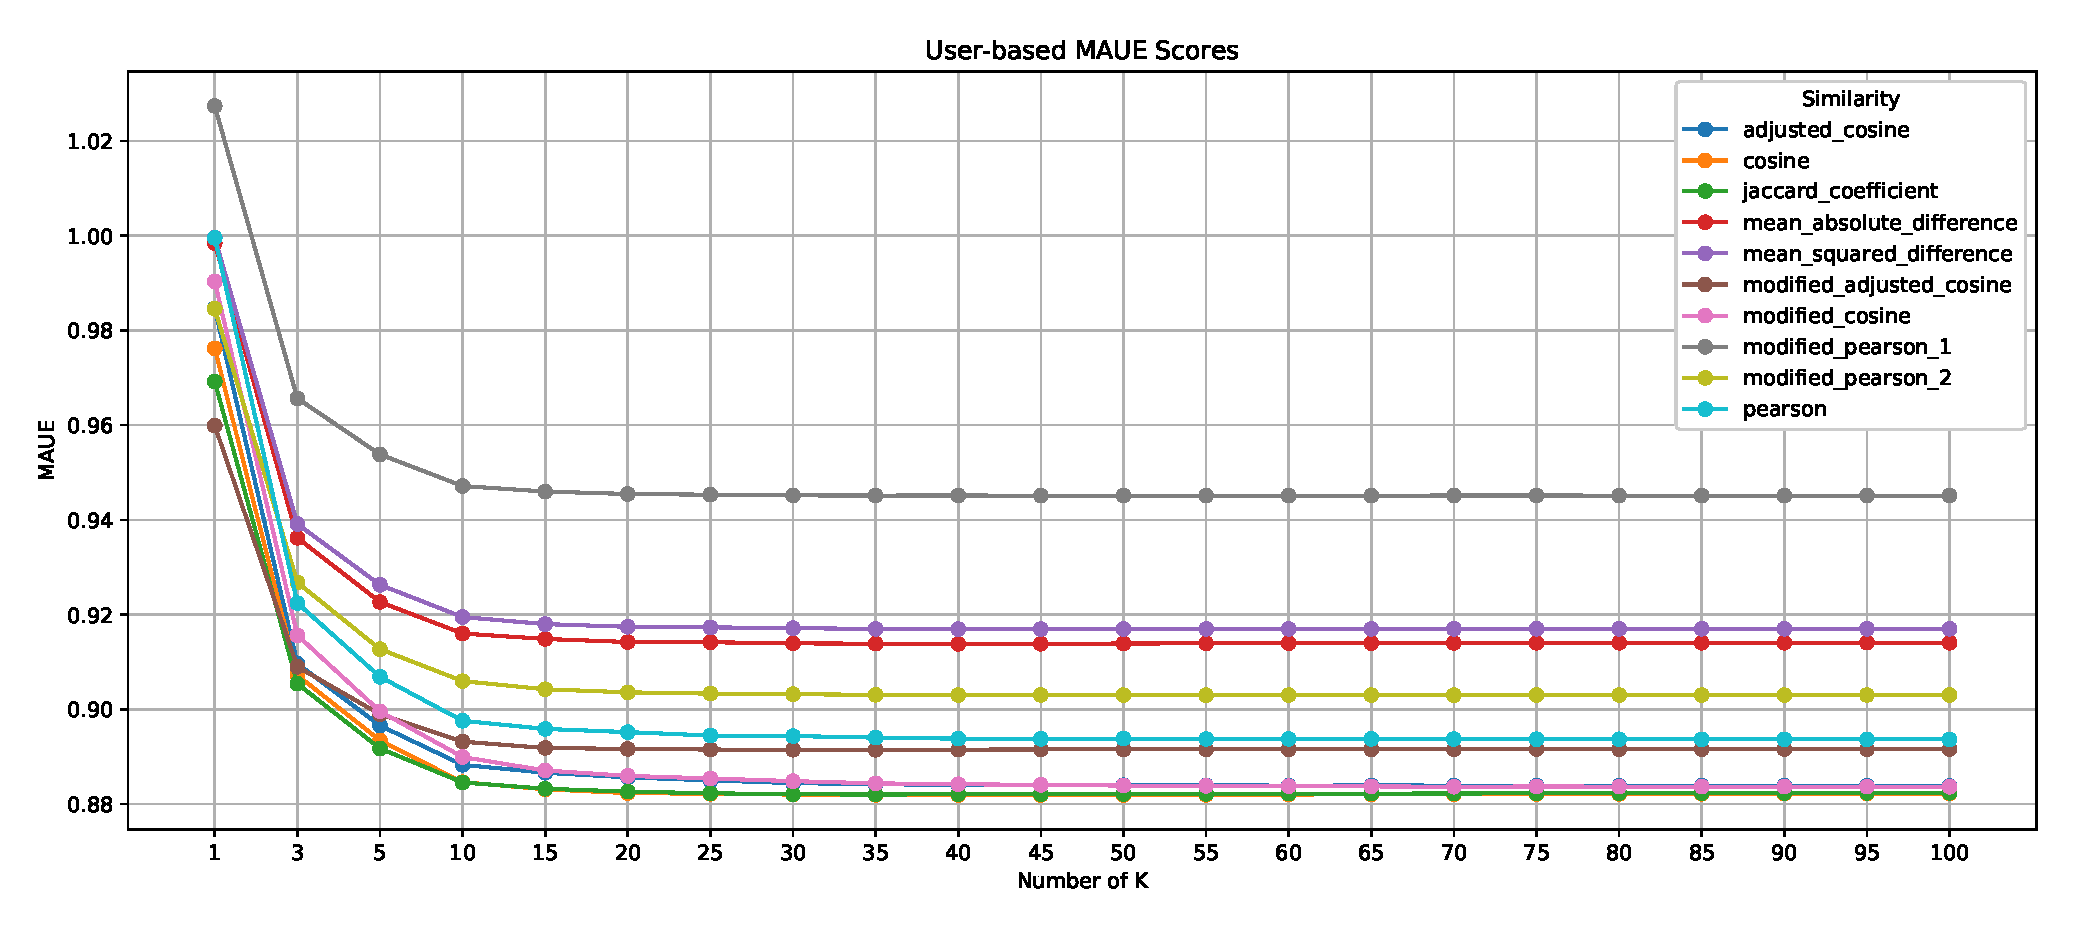
\includegraphics[width=1\textwidth]{chapter_4/knn/User_MAUE_KNN.eps}
\caption{User-based KNN MAUE scores}
\end{figure}

\subsection{RMSUE}

\begin{figure}[H]
\centering
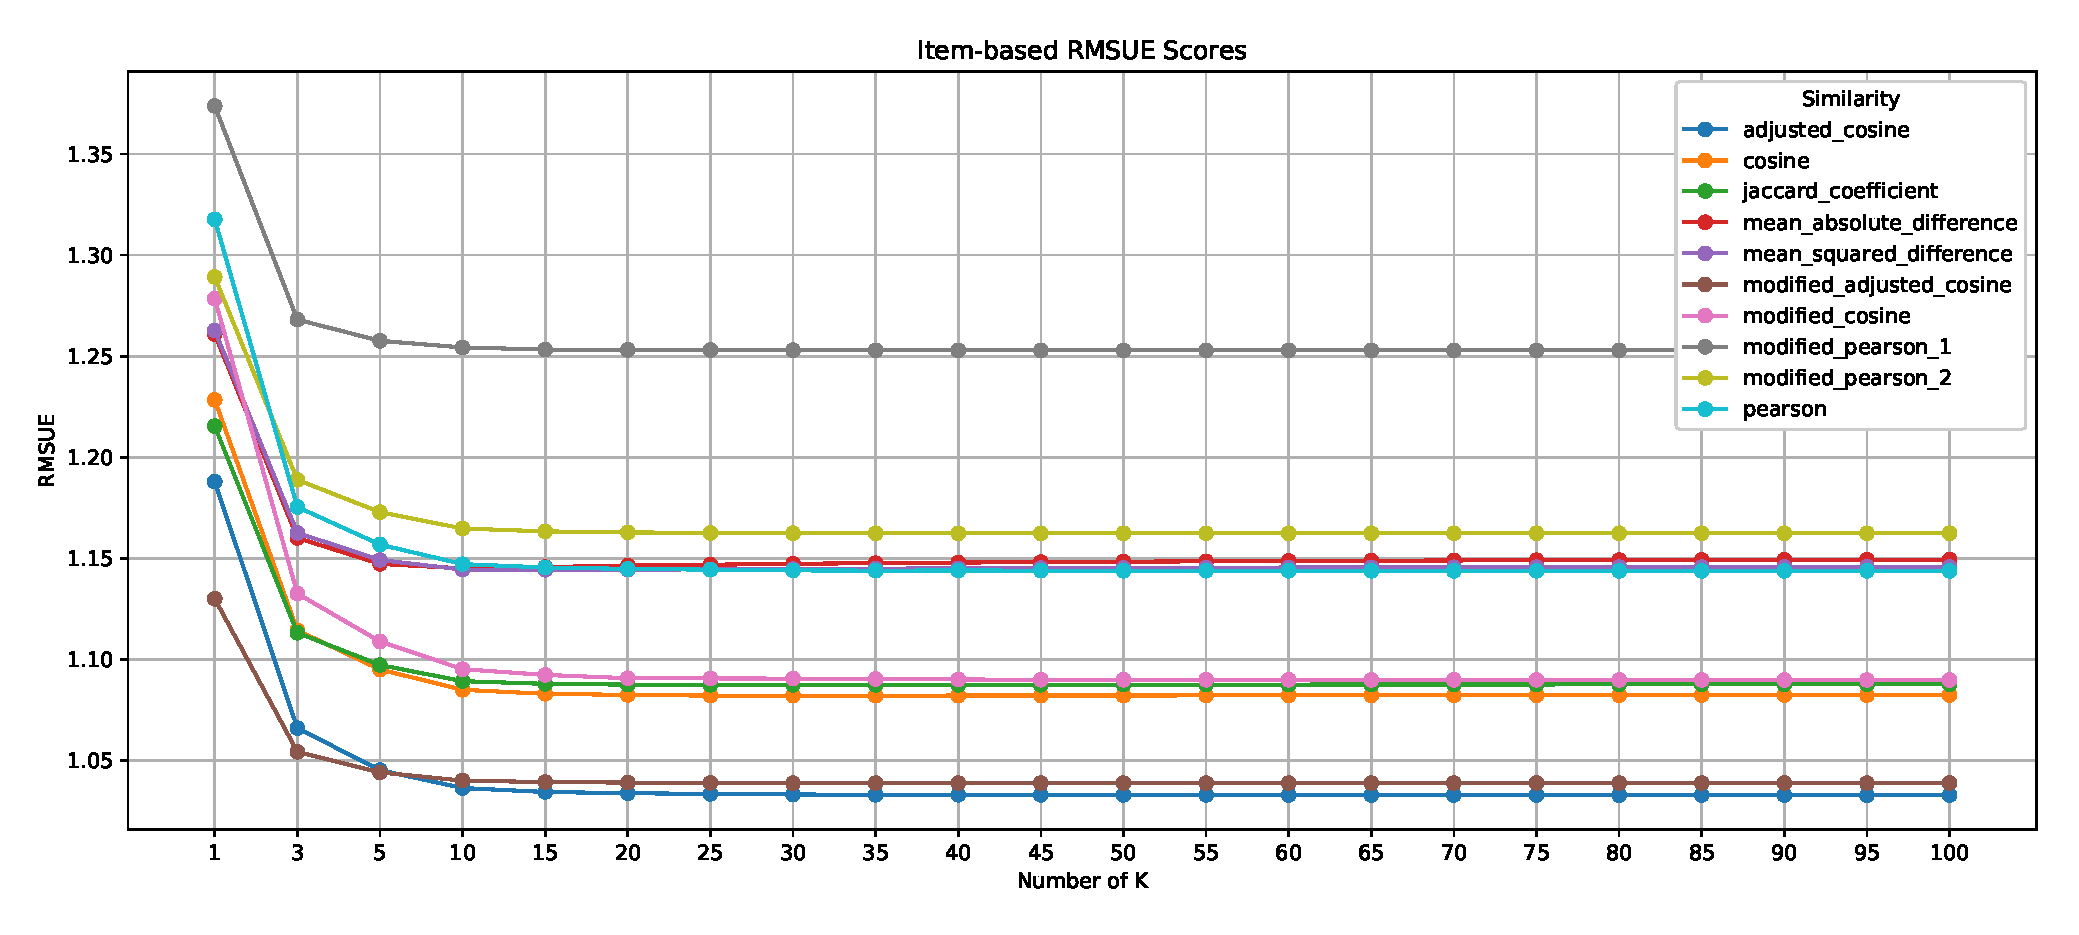
\includegraphics[width=1\textwidth]{chapter_4/knn/Item_RMSUE_KNN.eps}
\caption{Item-based KNN RMSUE scores}
\end{figure}

\begin{figure}[H]
\centering
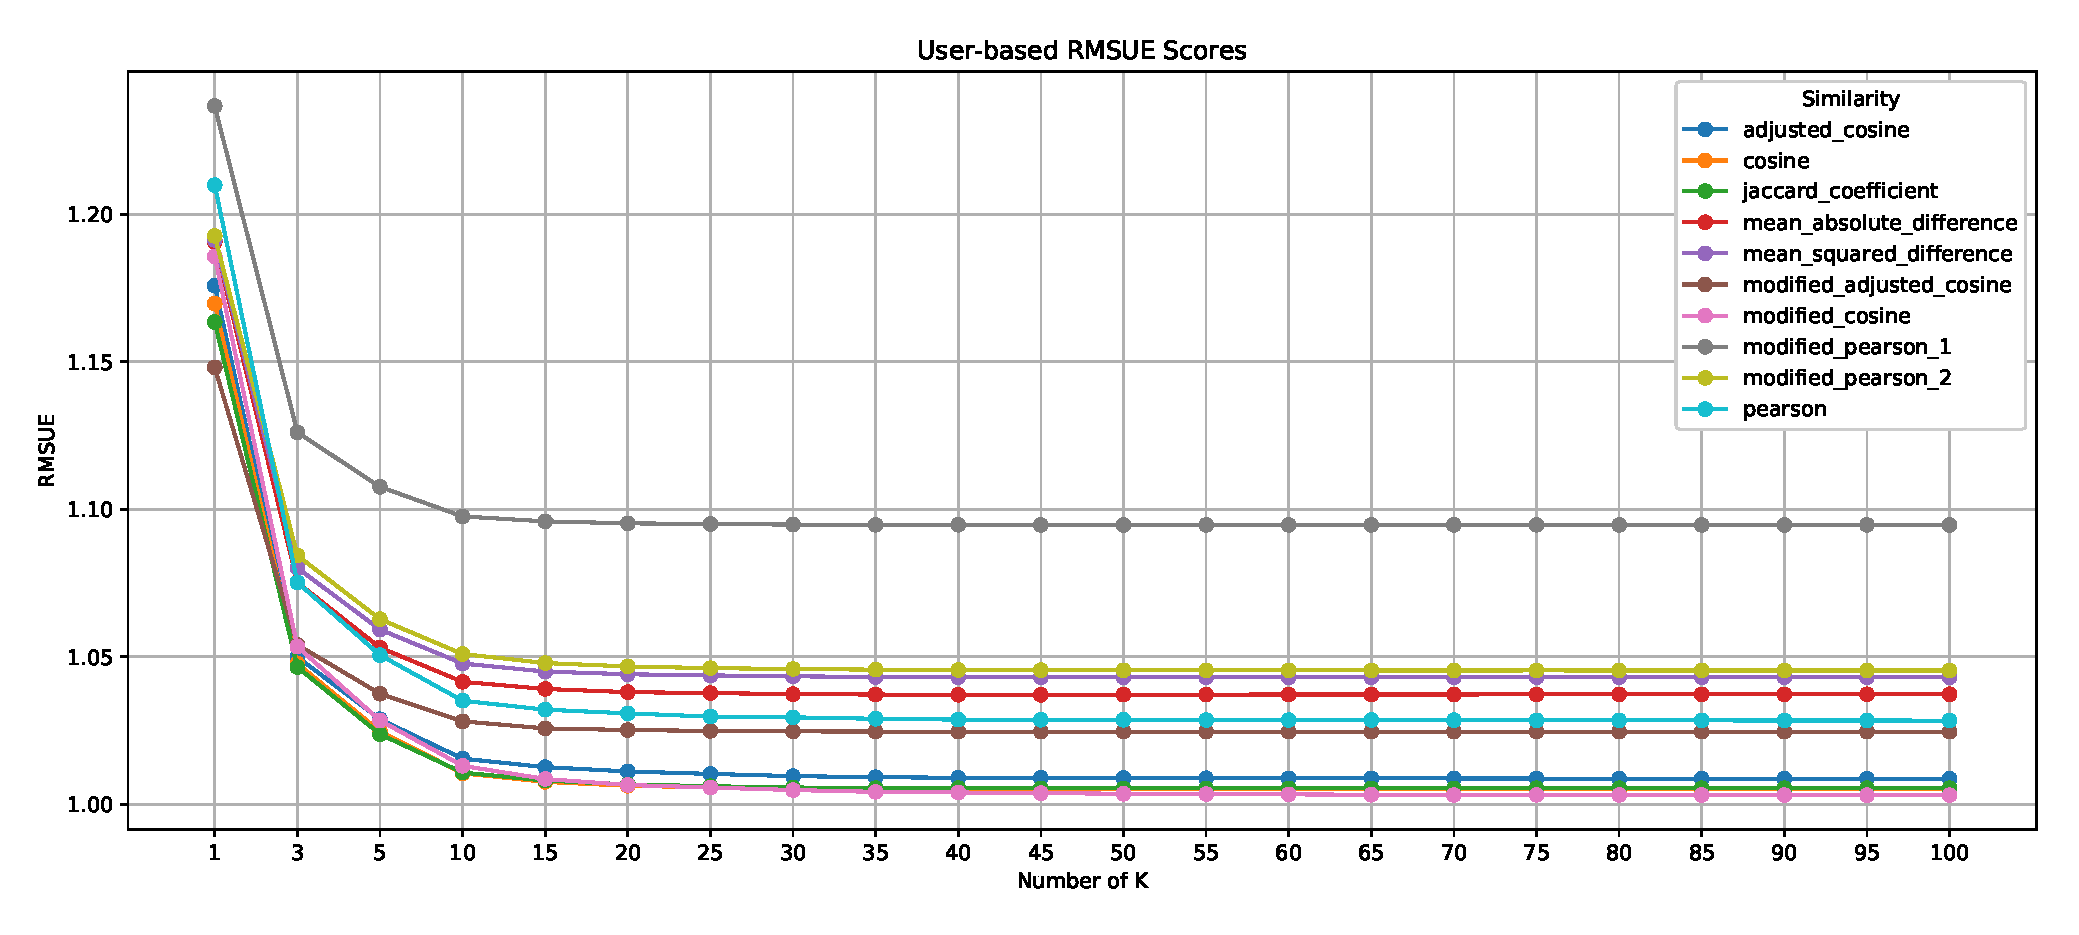
\includegraphics[width=1\textwidth]{chapter_4/knn/User_RMSUE_KNN.eps}
\caption{User-based KNN RMSUE scores}
\end{figure}

\section{Recursive-KNN Scores}

\subsection{MAE}

\subsubsection{Item-Based}

\begin{figure}[H]
\centering
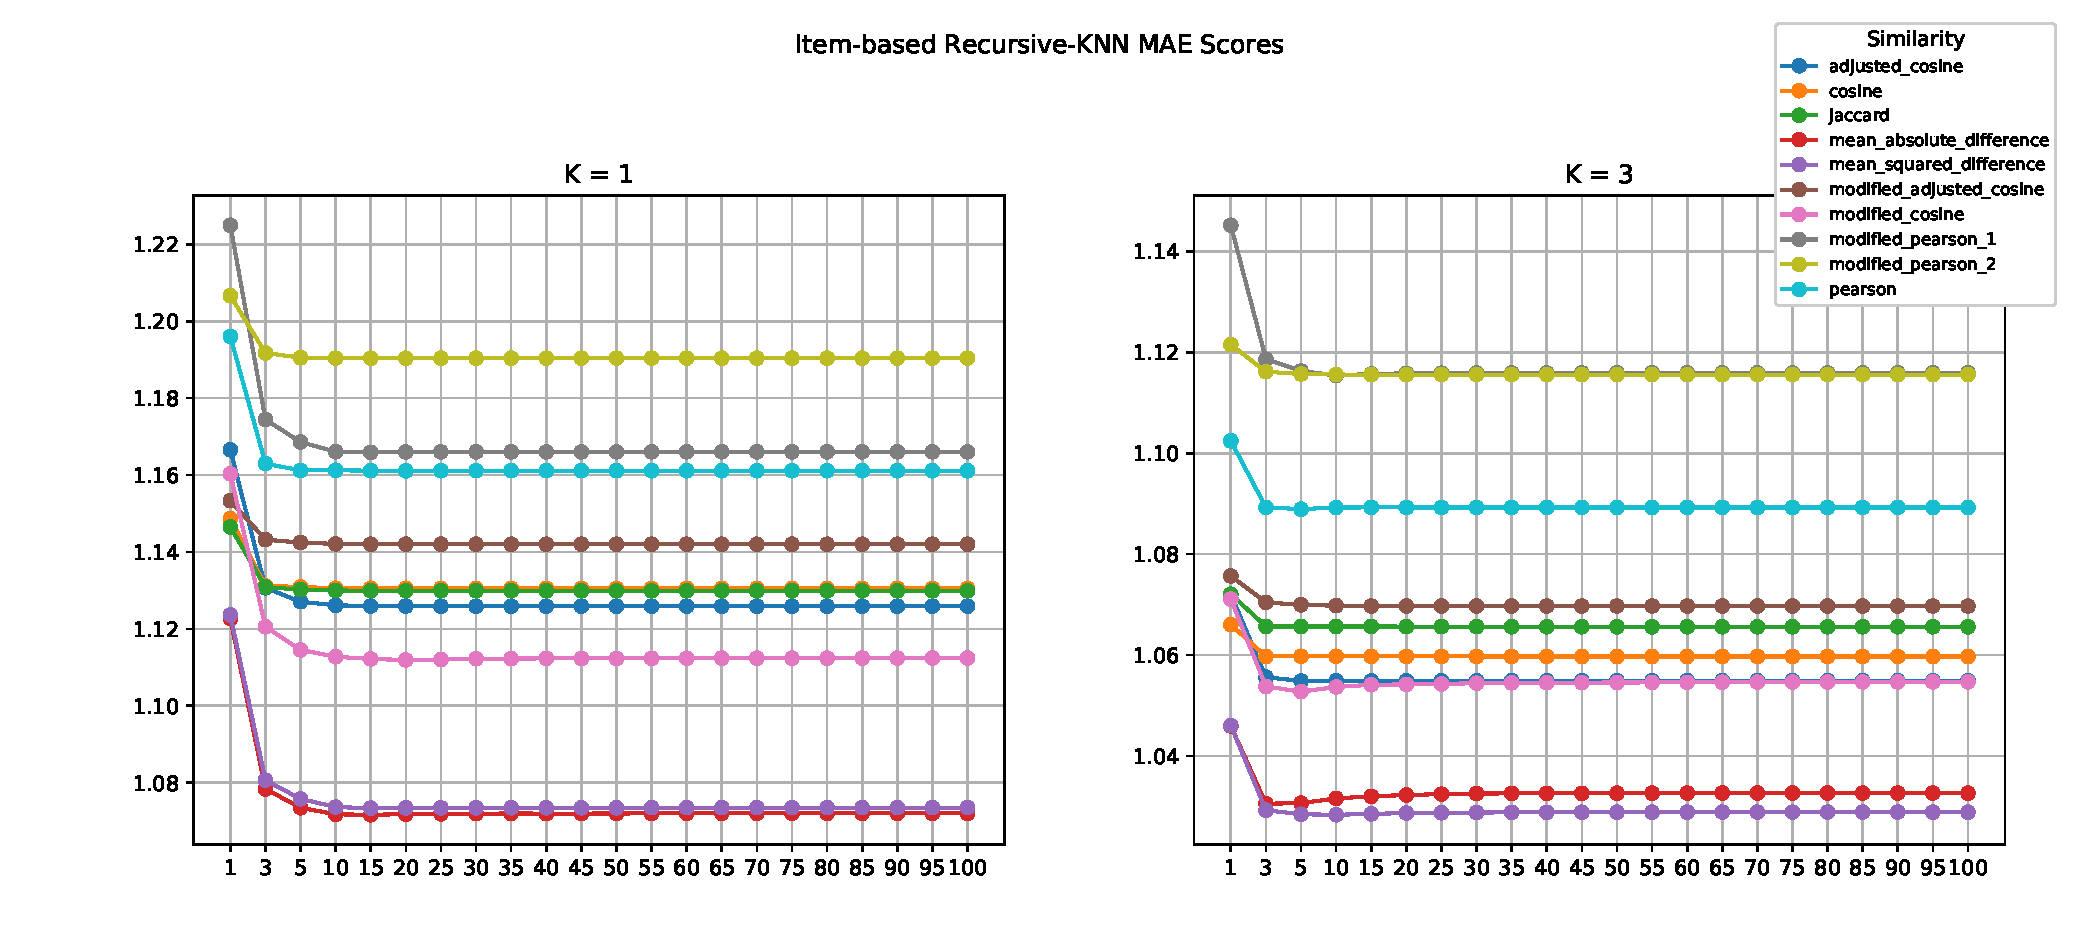
\includegraphics[width=1\textwidth]{chapter_4/rknn/mae/item_1_3.eps}
\caption{Item-based RKNN MAE scores}
\end{figure}

\begin{figure}[H]
\centering
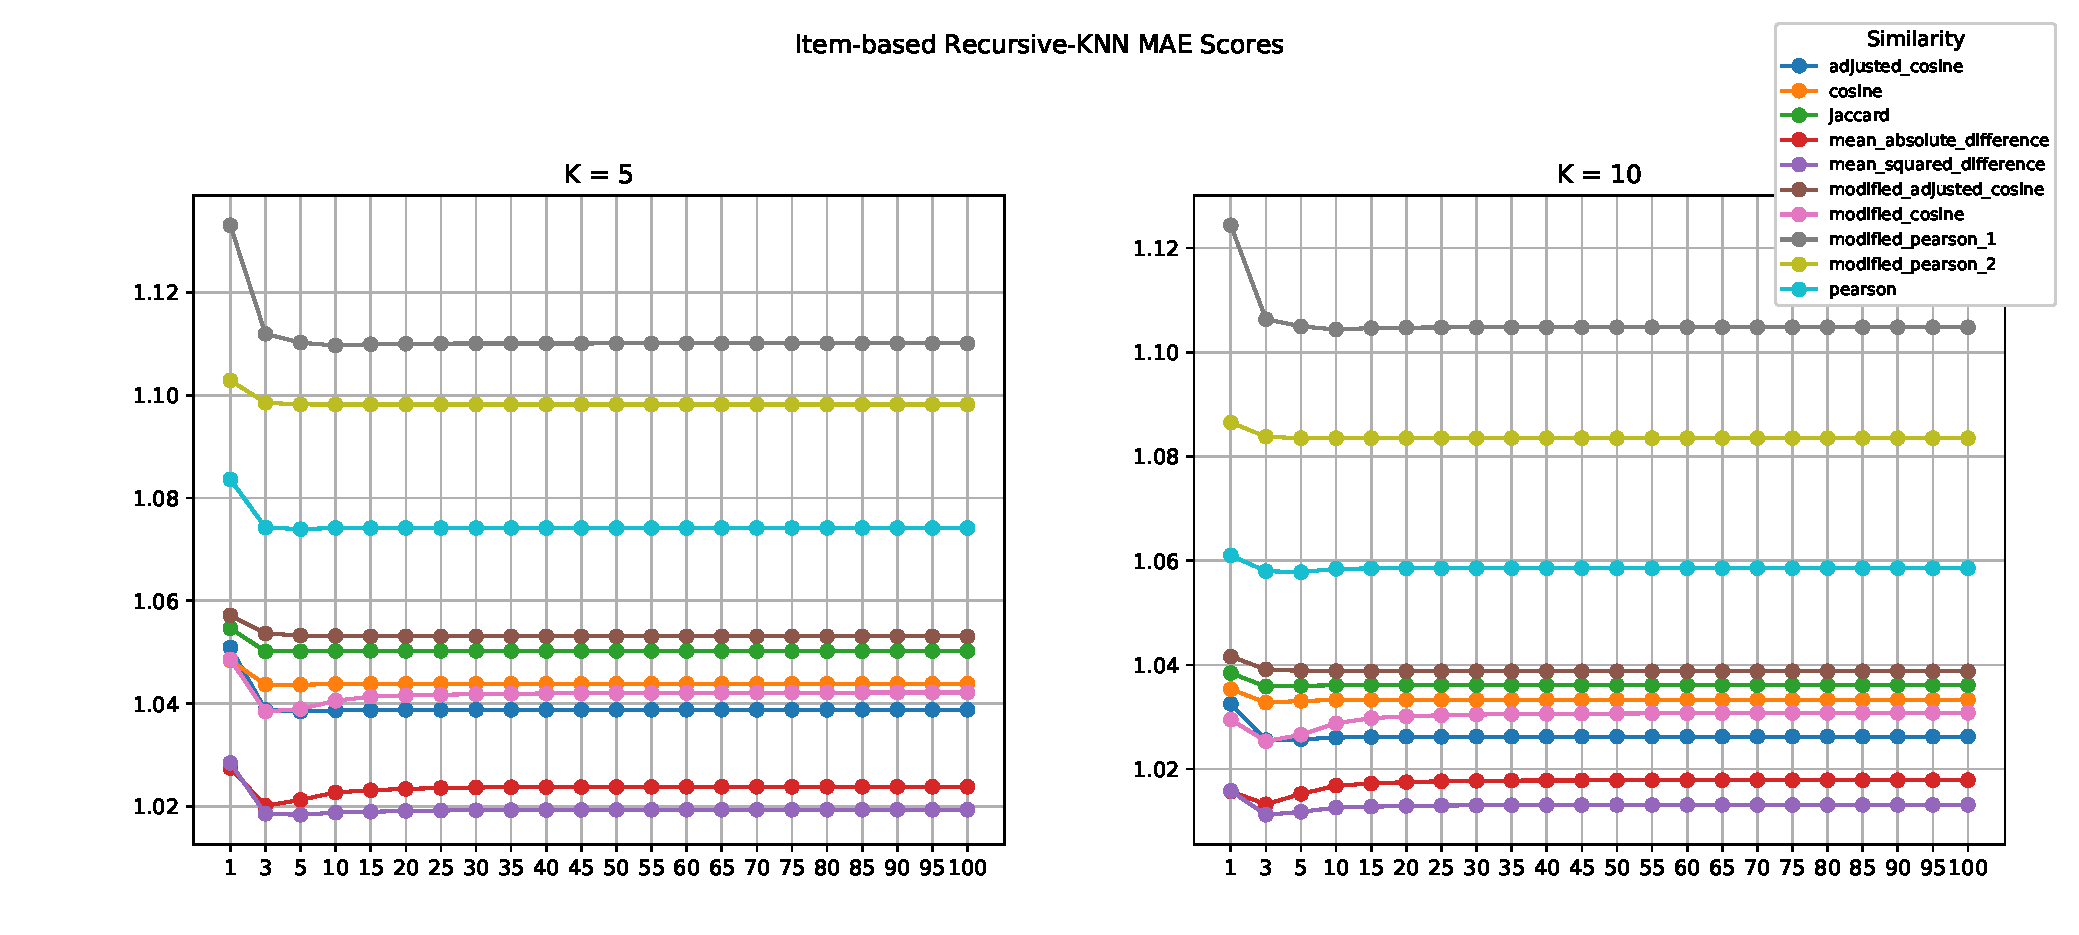
\includegraphics[width=1\textwidth]{chapter_4/rknn/mae/item_5_10.eps}
\caption{Item-based RKNN MAE scores}
\end{figure}

\begin{figure}[H]
\centering
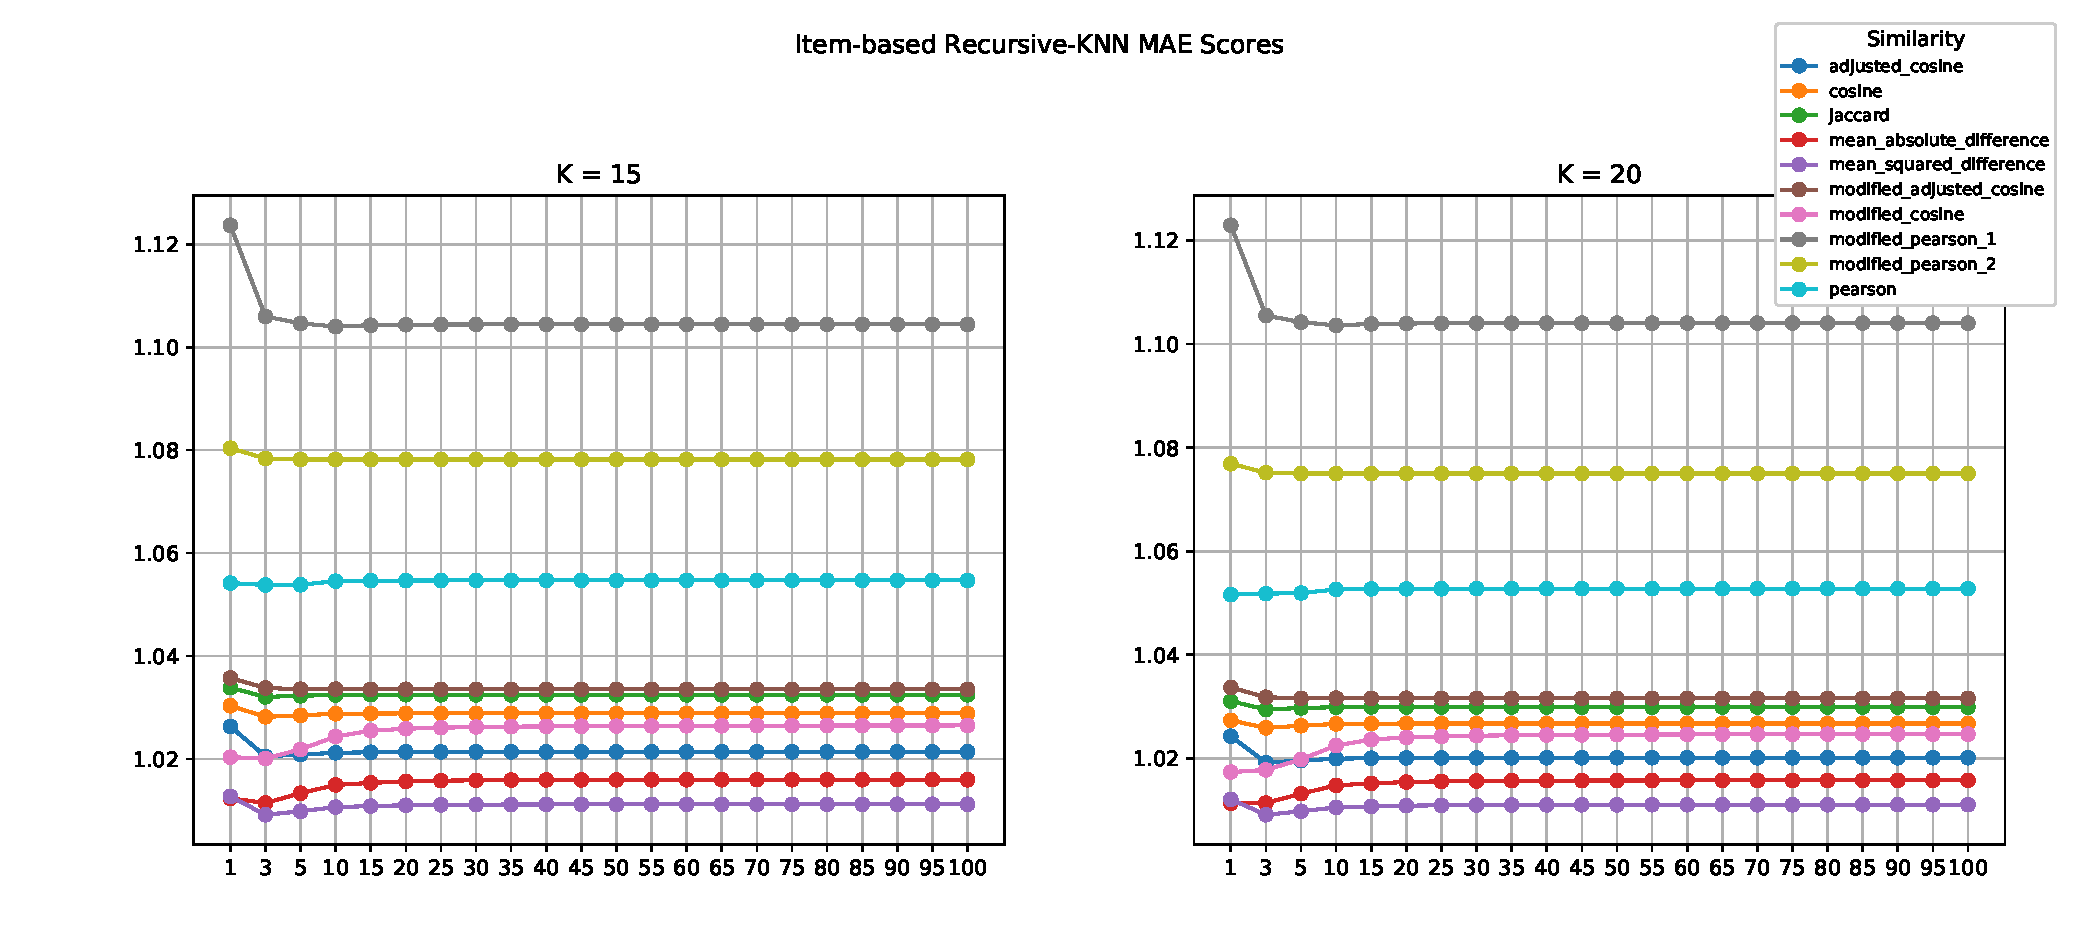
\includegraphics[width=1\textwidth]{chapter_4/rknn/mae/item_15_20.eps}
\caption{Item-based RKNN MAE scores}
\end{figure}

\begin{figure}[H]
\centering
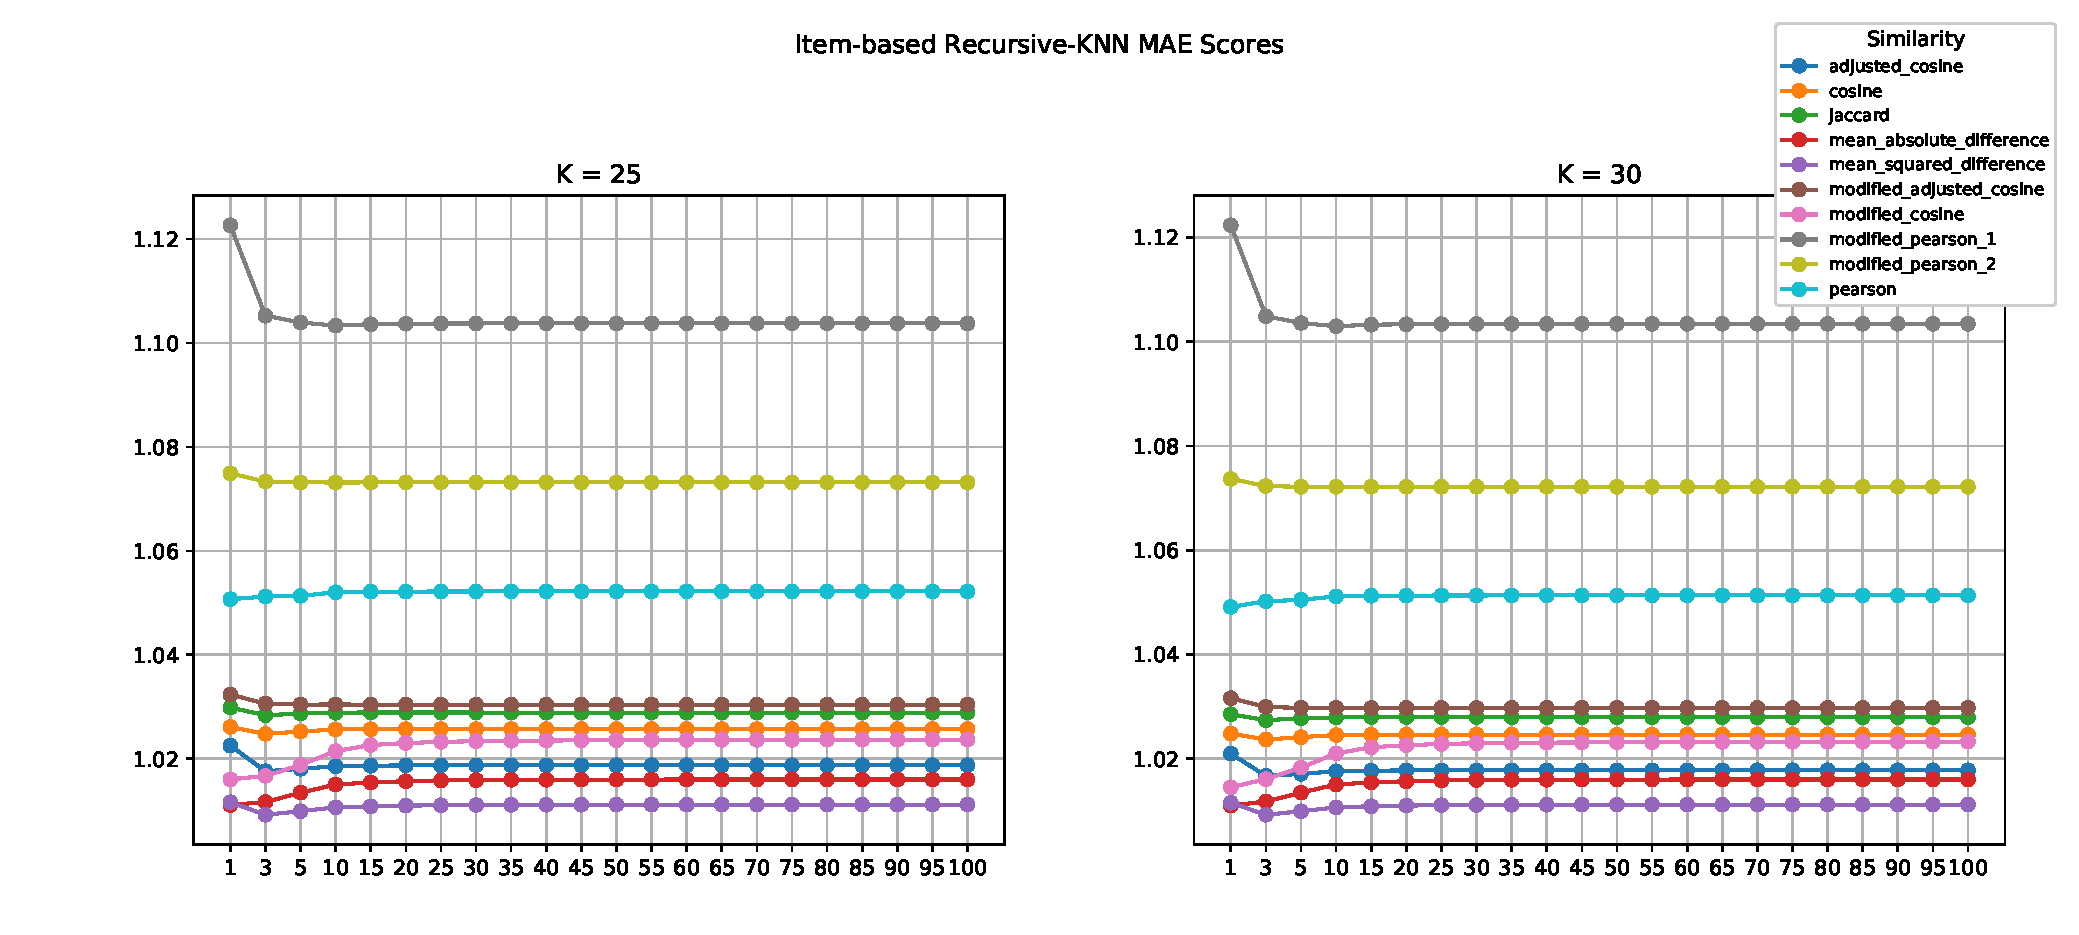
\includegraphics[width=1\textwidth]{chapter_4/rknn/mae/item_25_30.eps}
\caption{Item-based RKNN MAE scores}
\end{figure}

\begin{figure}[H]
\centering
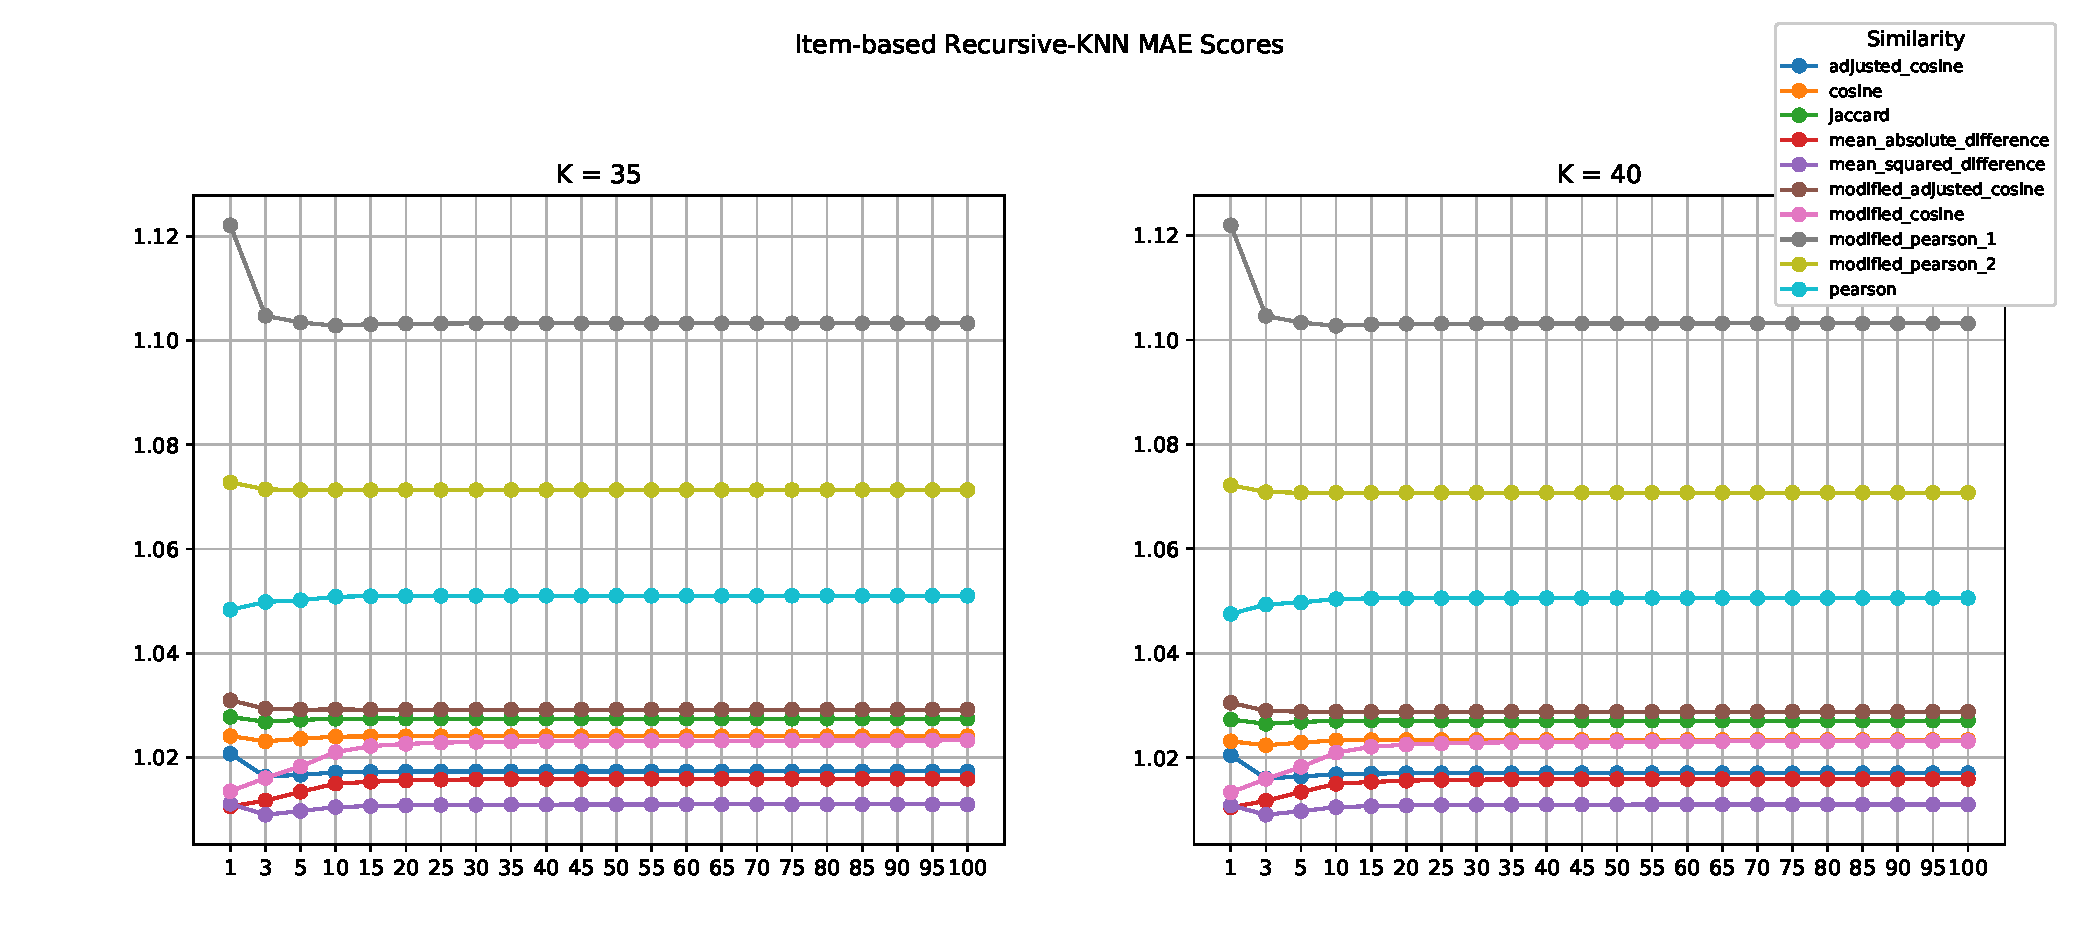
\includegraphics[width=1\textwidth]{chapter_4/rknn/mae/item_35_40.eps}
\caption{Item-based RKNN MAE scores}
\end{figure}

\begin{figure}[H]
\centering
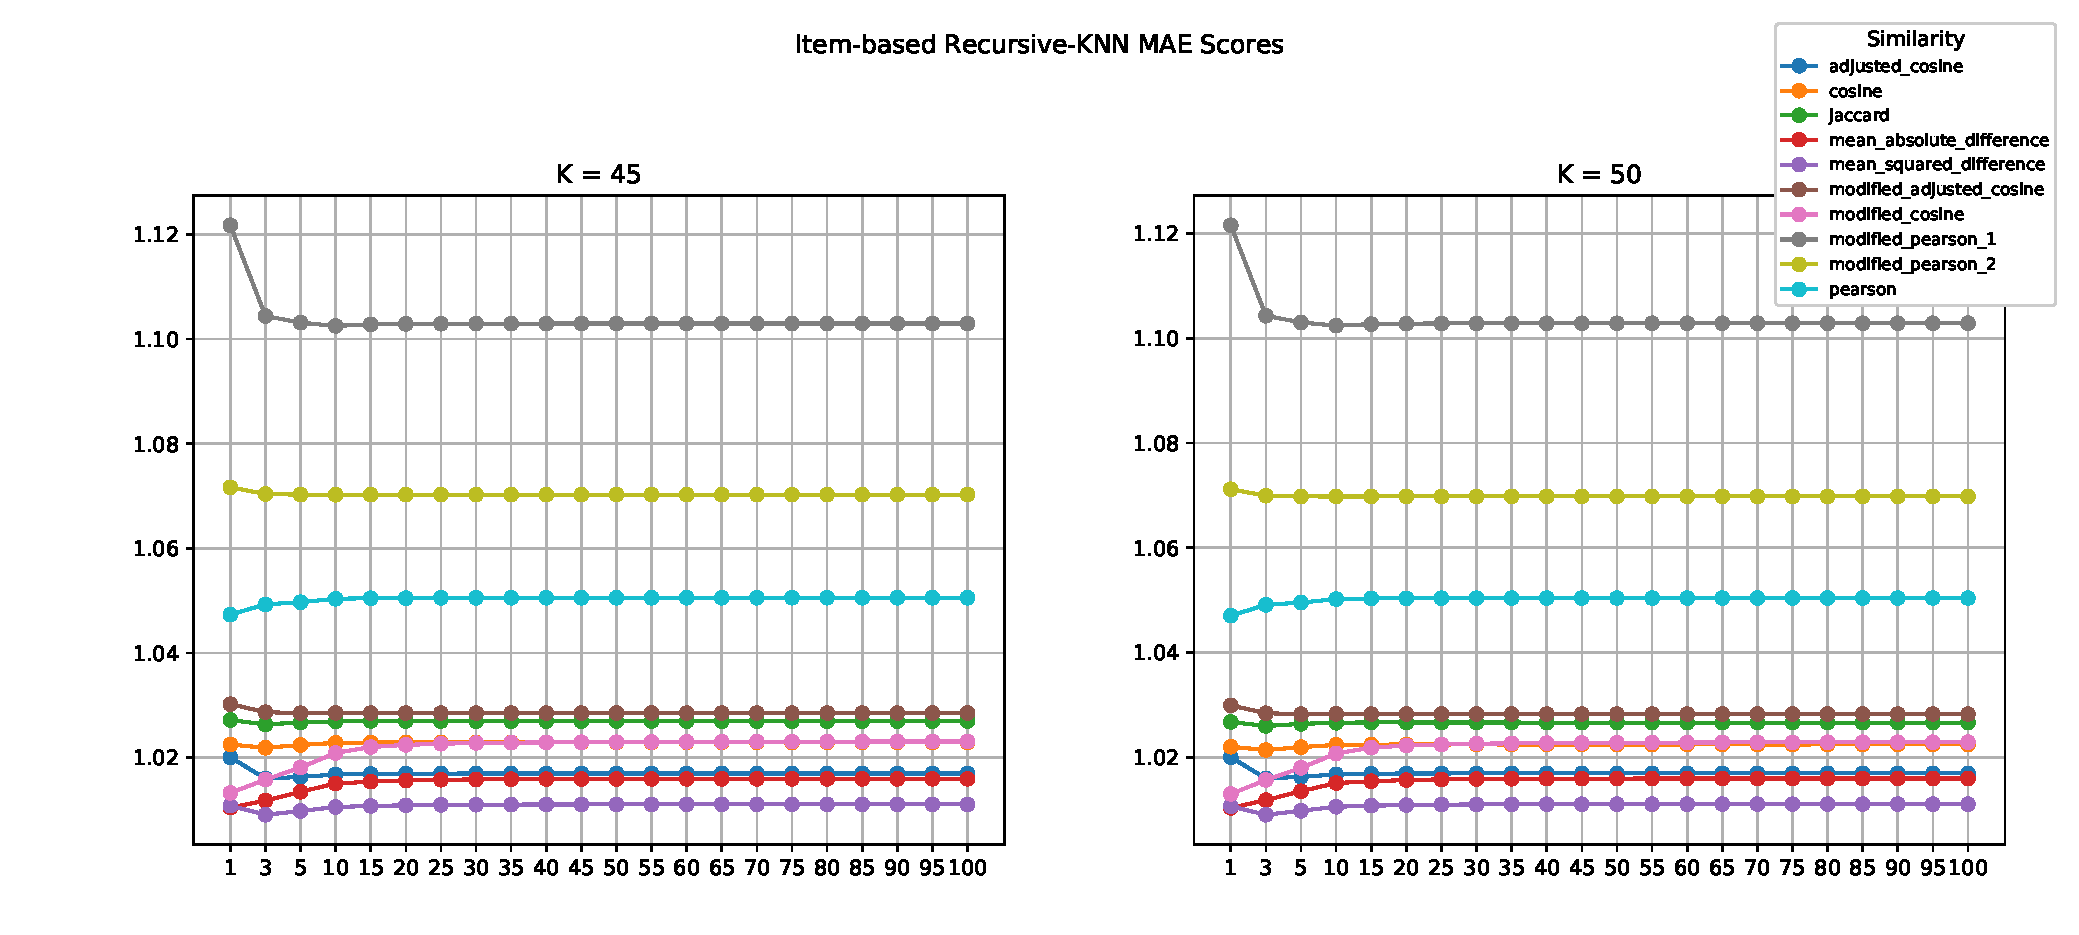
\includegraphics[width=1\textwidth]{chapter_4/rknn/mae/item_45_50.eps}
\caption{Item-based RKNN MAE scores}
\end{figure}

\begin{figure}[H]
\centering
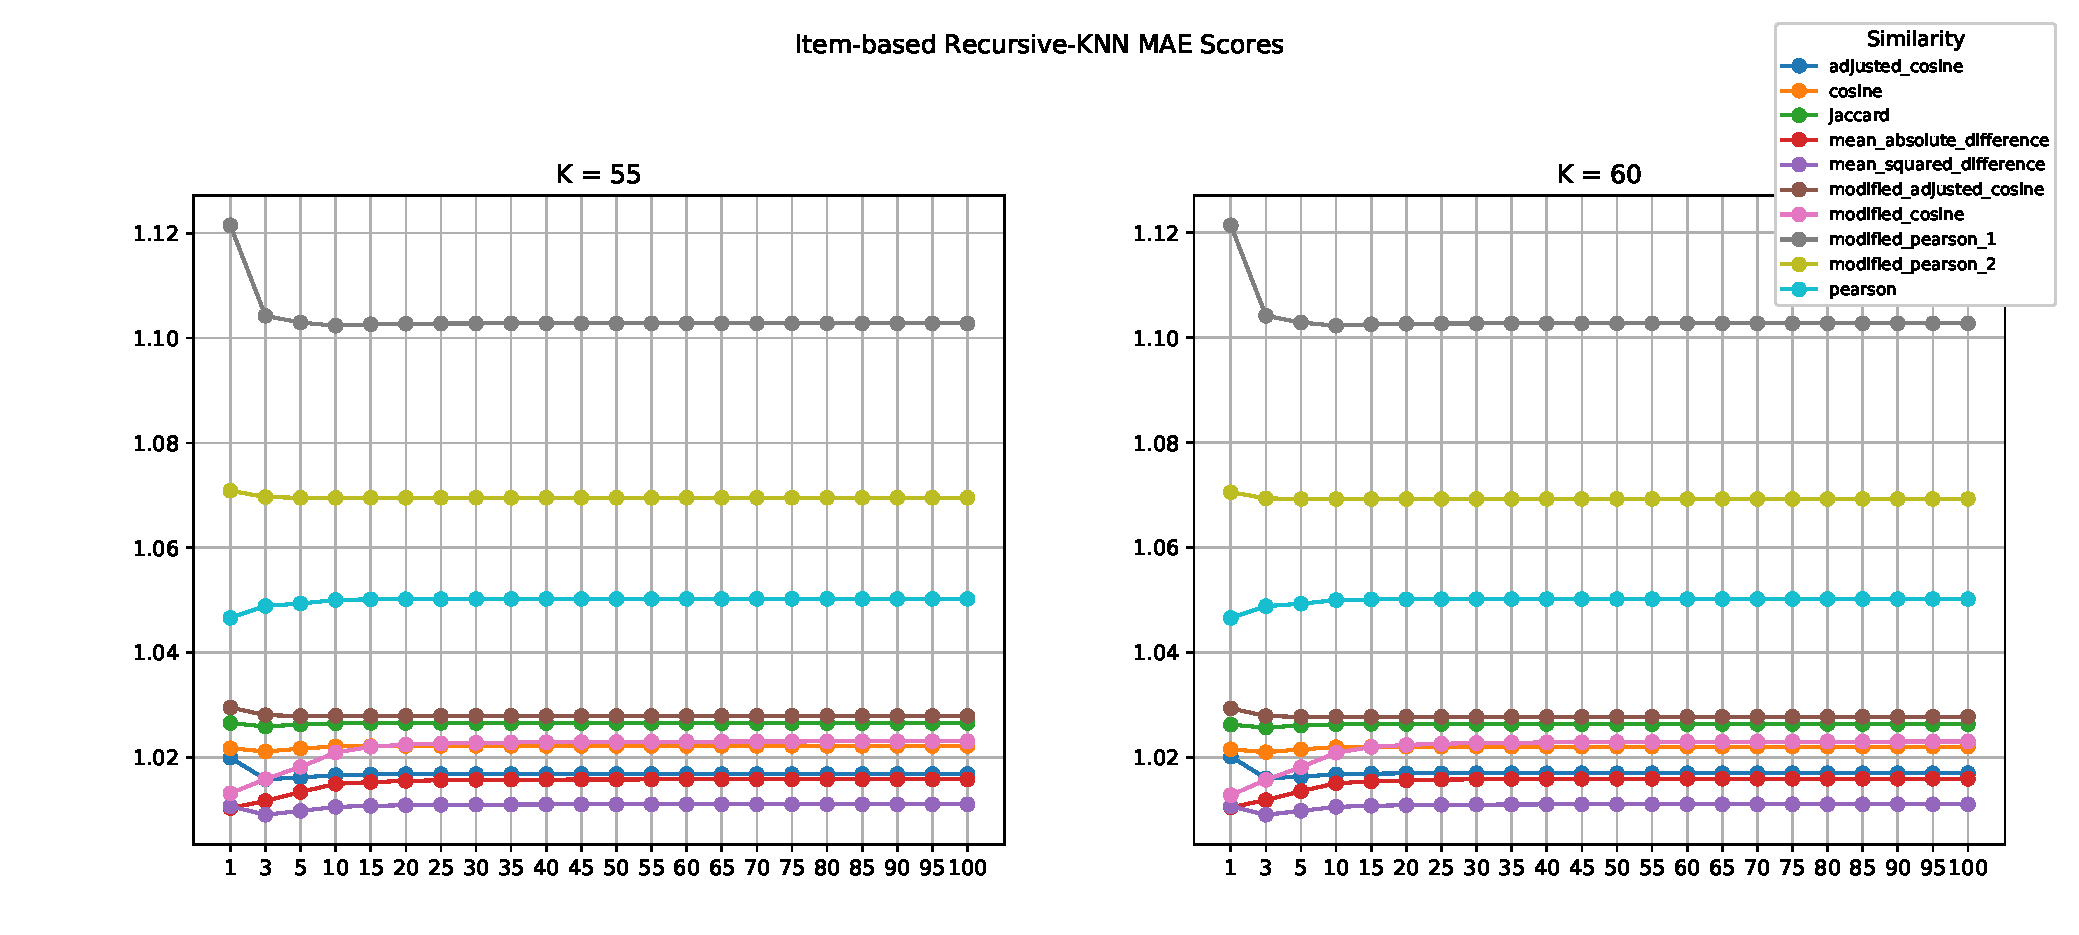
\includegraphics[width=1\textwidth]{chapter_4/rknn/mae/item_55_60.eps}
\caption{Item-based RKNN MAE scores}
\end{figure}

\begin{figure}[H]
\centering
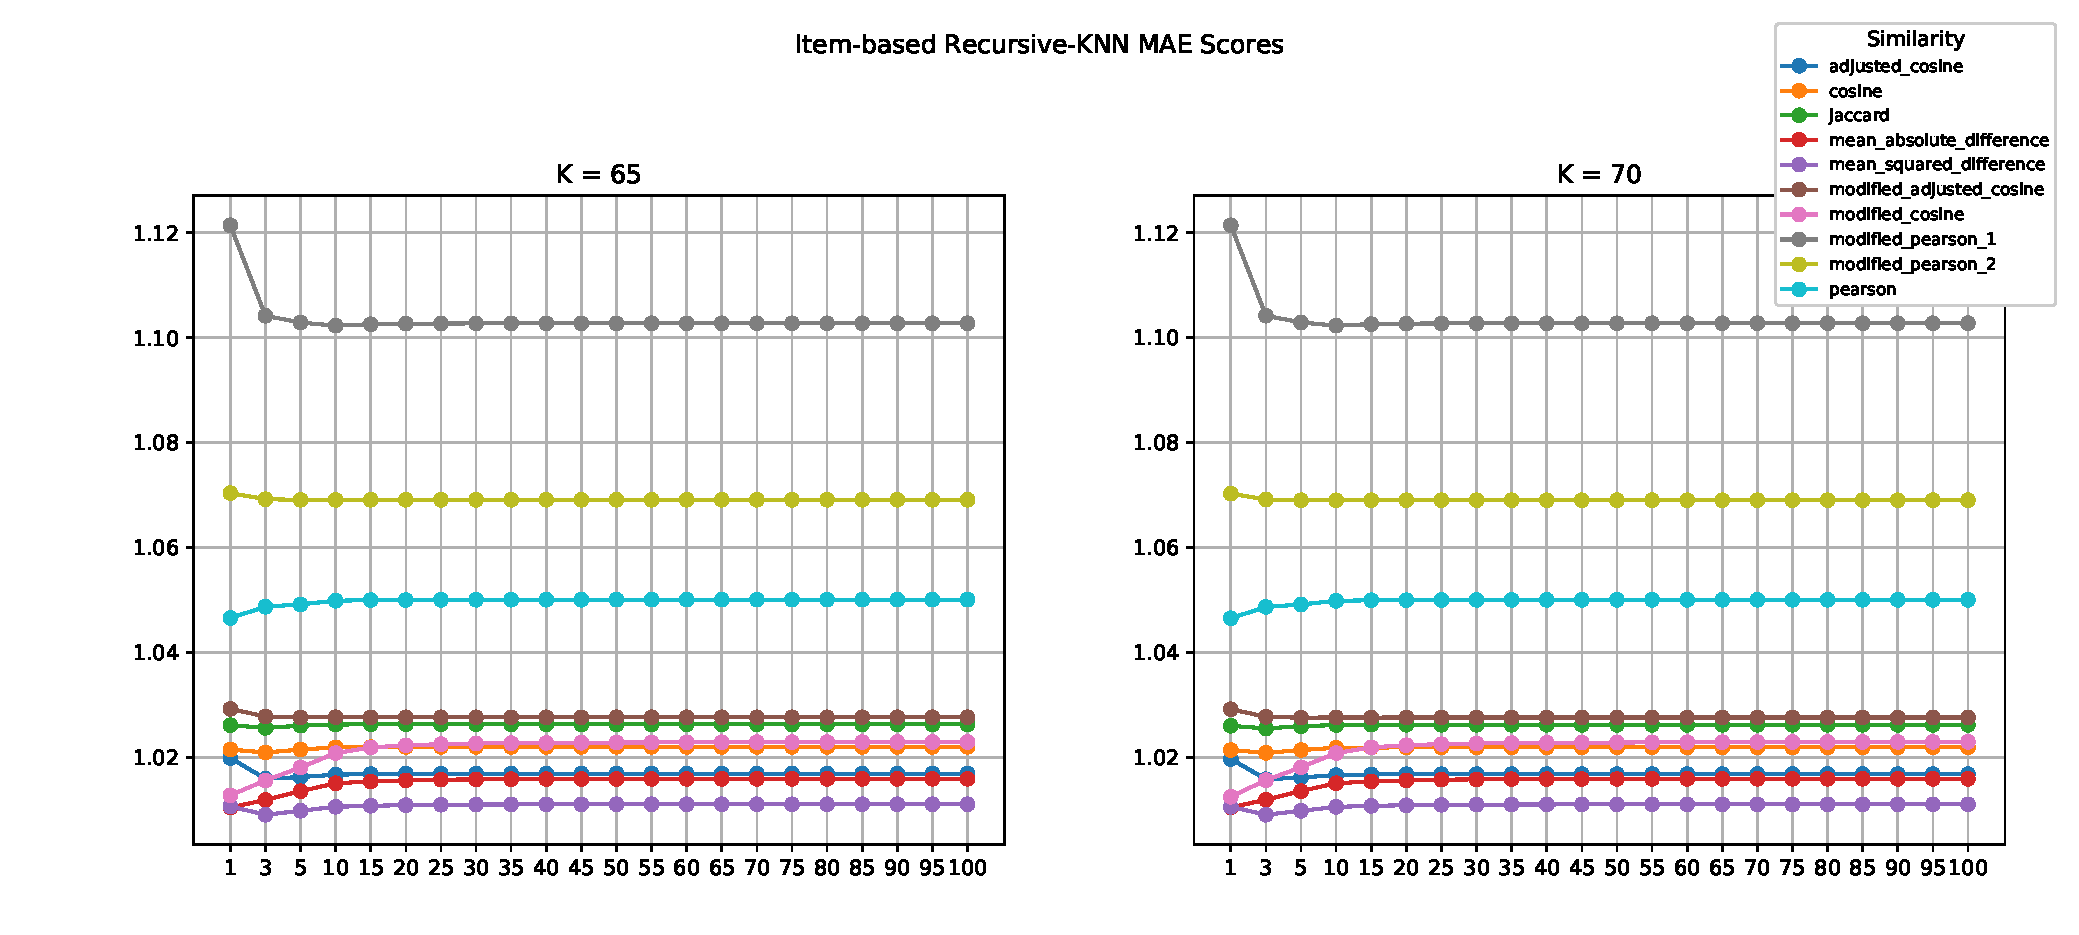
\includegraphics[width=1\textwidth]{chapter_4/rknn/mae/item_65_70.eps}
\caption{Item-based RKNN MAE scores}
\end{figure}

\begin{figure}[H]
\centering
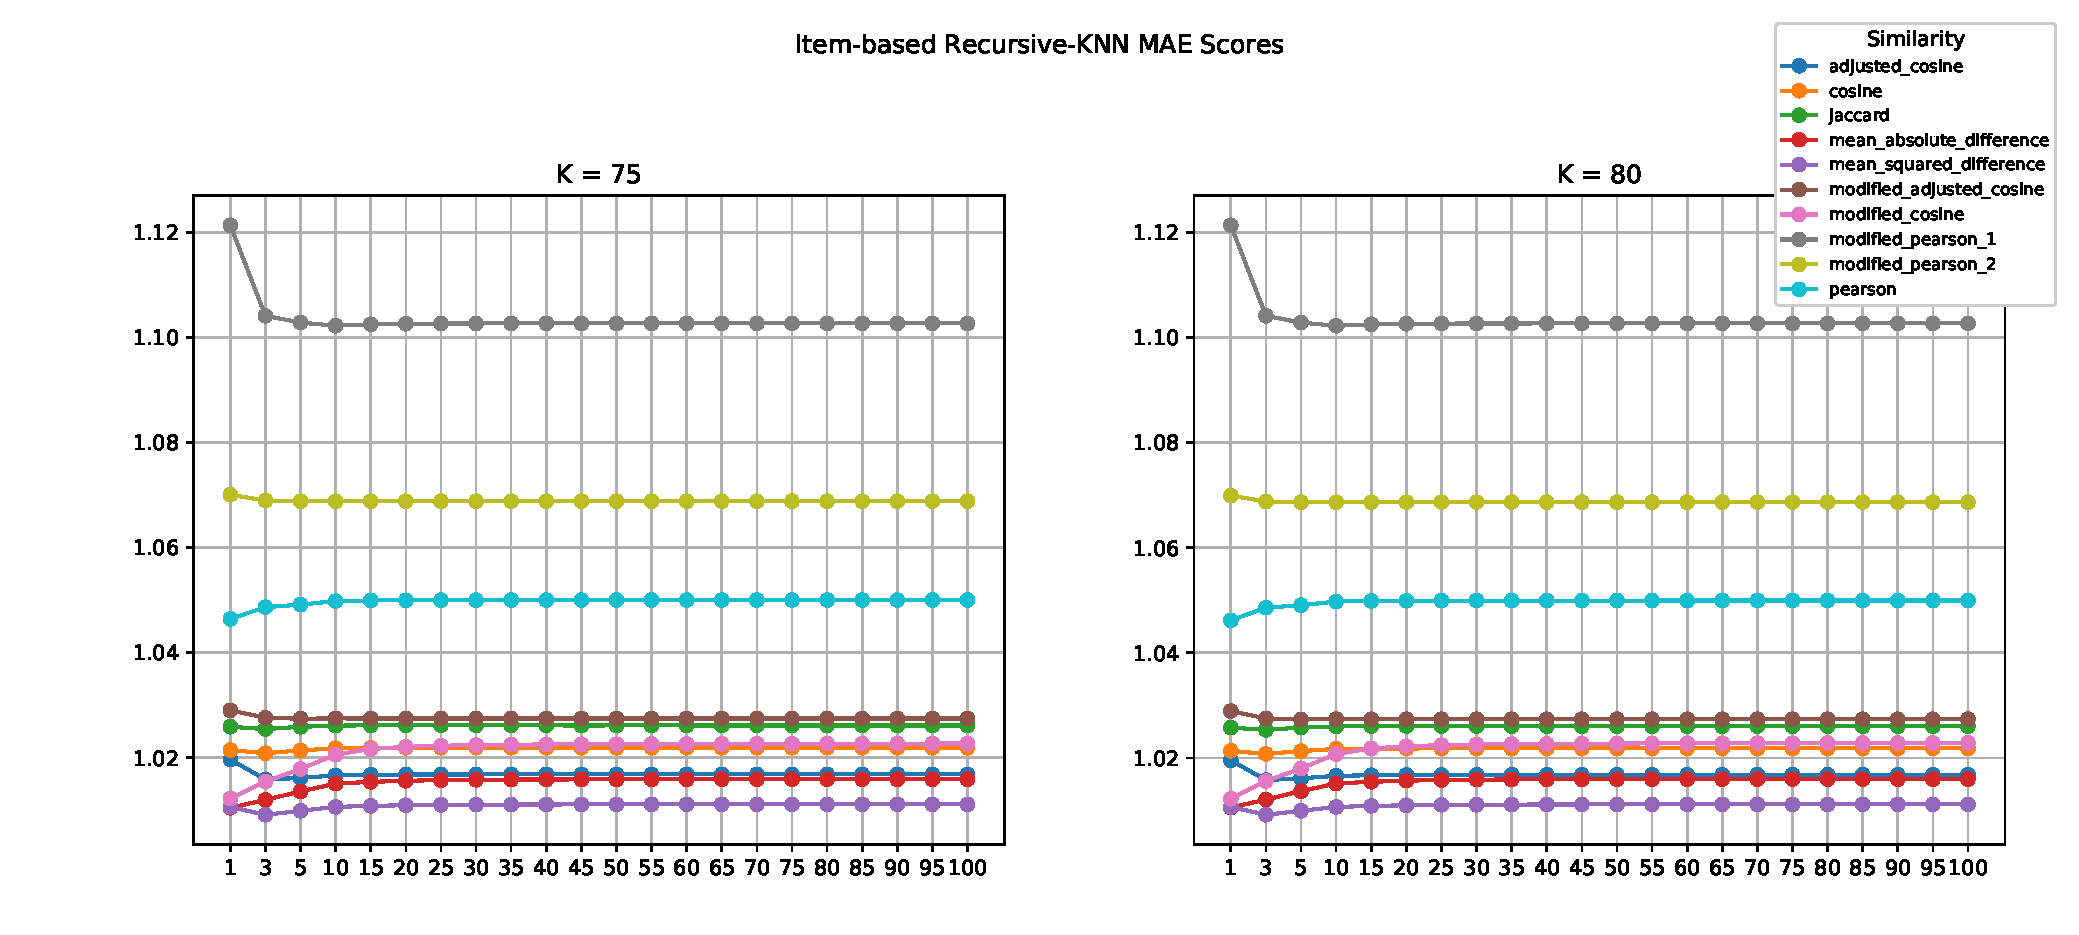
\includegraphics[width=1\textwidth]{chapter_4/rknn/mae/item_75_80.eps}
\caption{Item-based RKNN MAE scores}
\end{figure}

\begin{figure}[H]
\centering
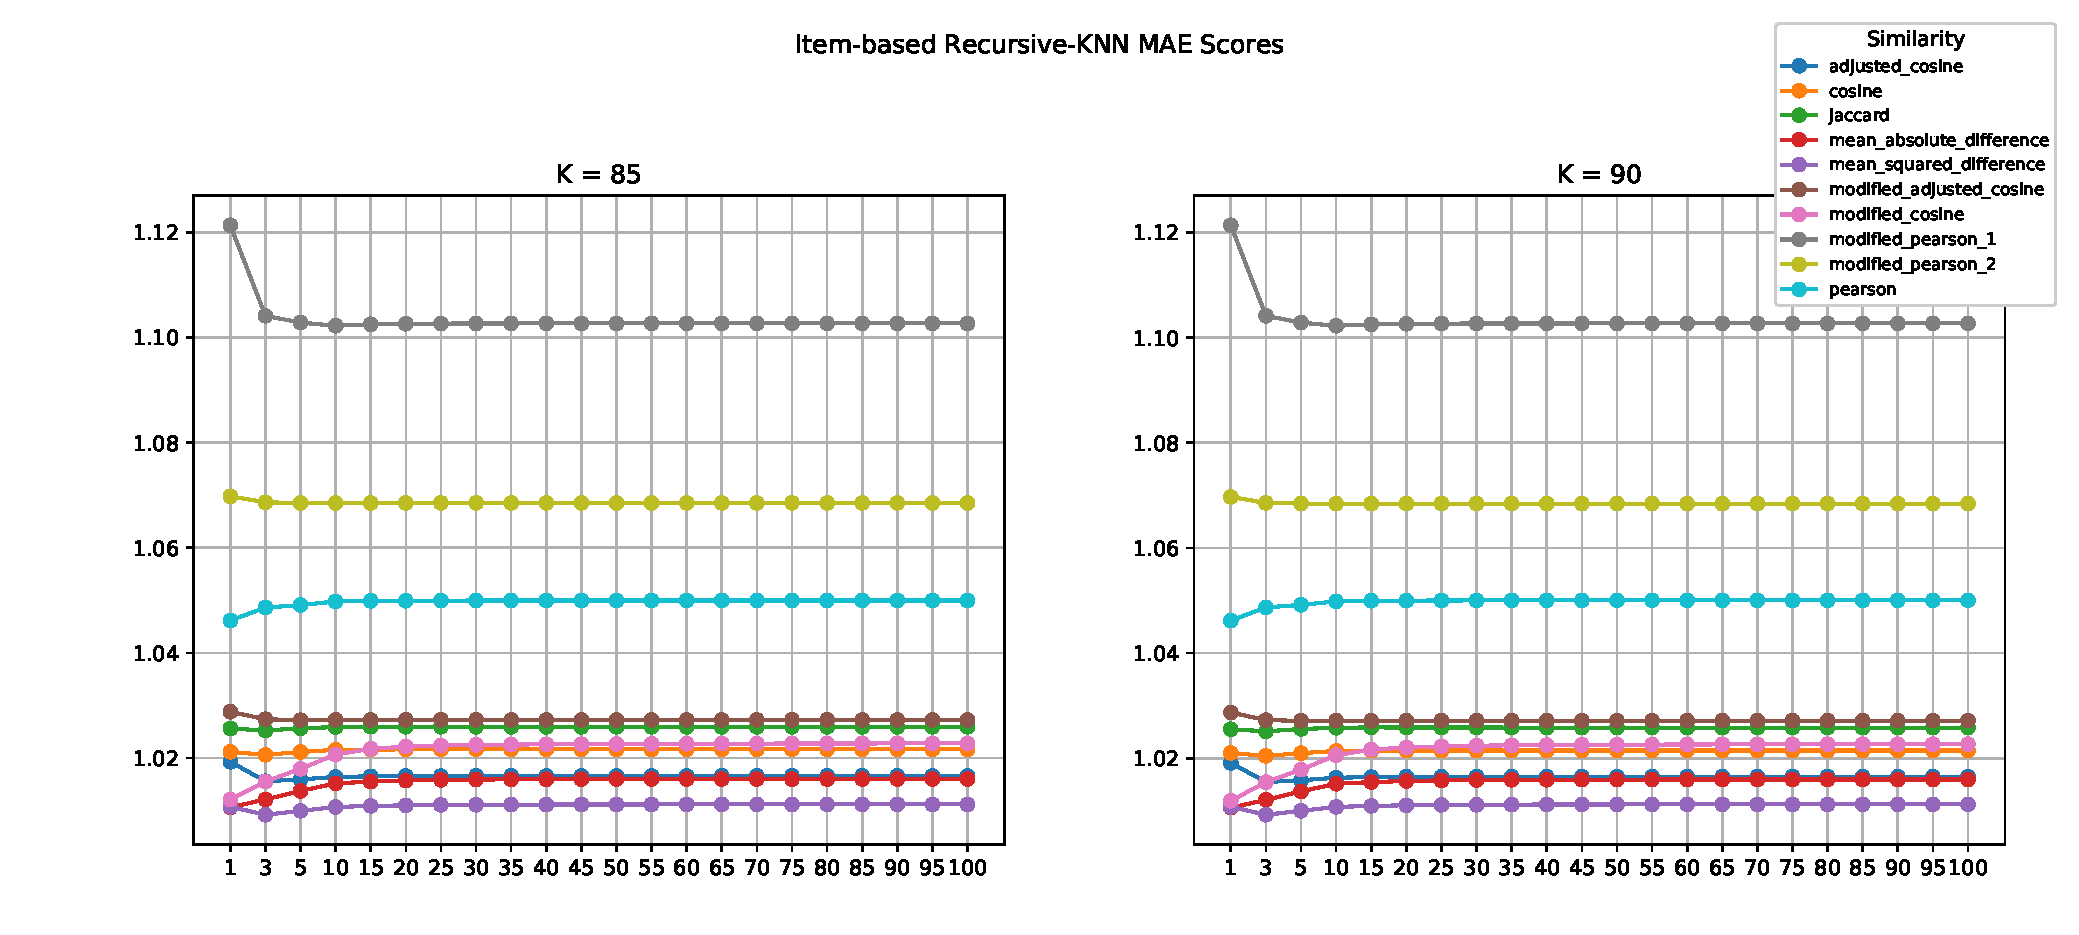
\includegraphics[width=1\textwidth]{chapter_4/rknn/mae/item_85_90.eps}
\caption{Item-based RKNN MAE scores}
\end{figure}

\begin{figure}[H]
\centering
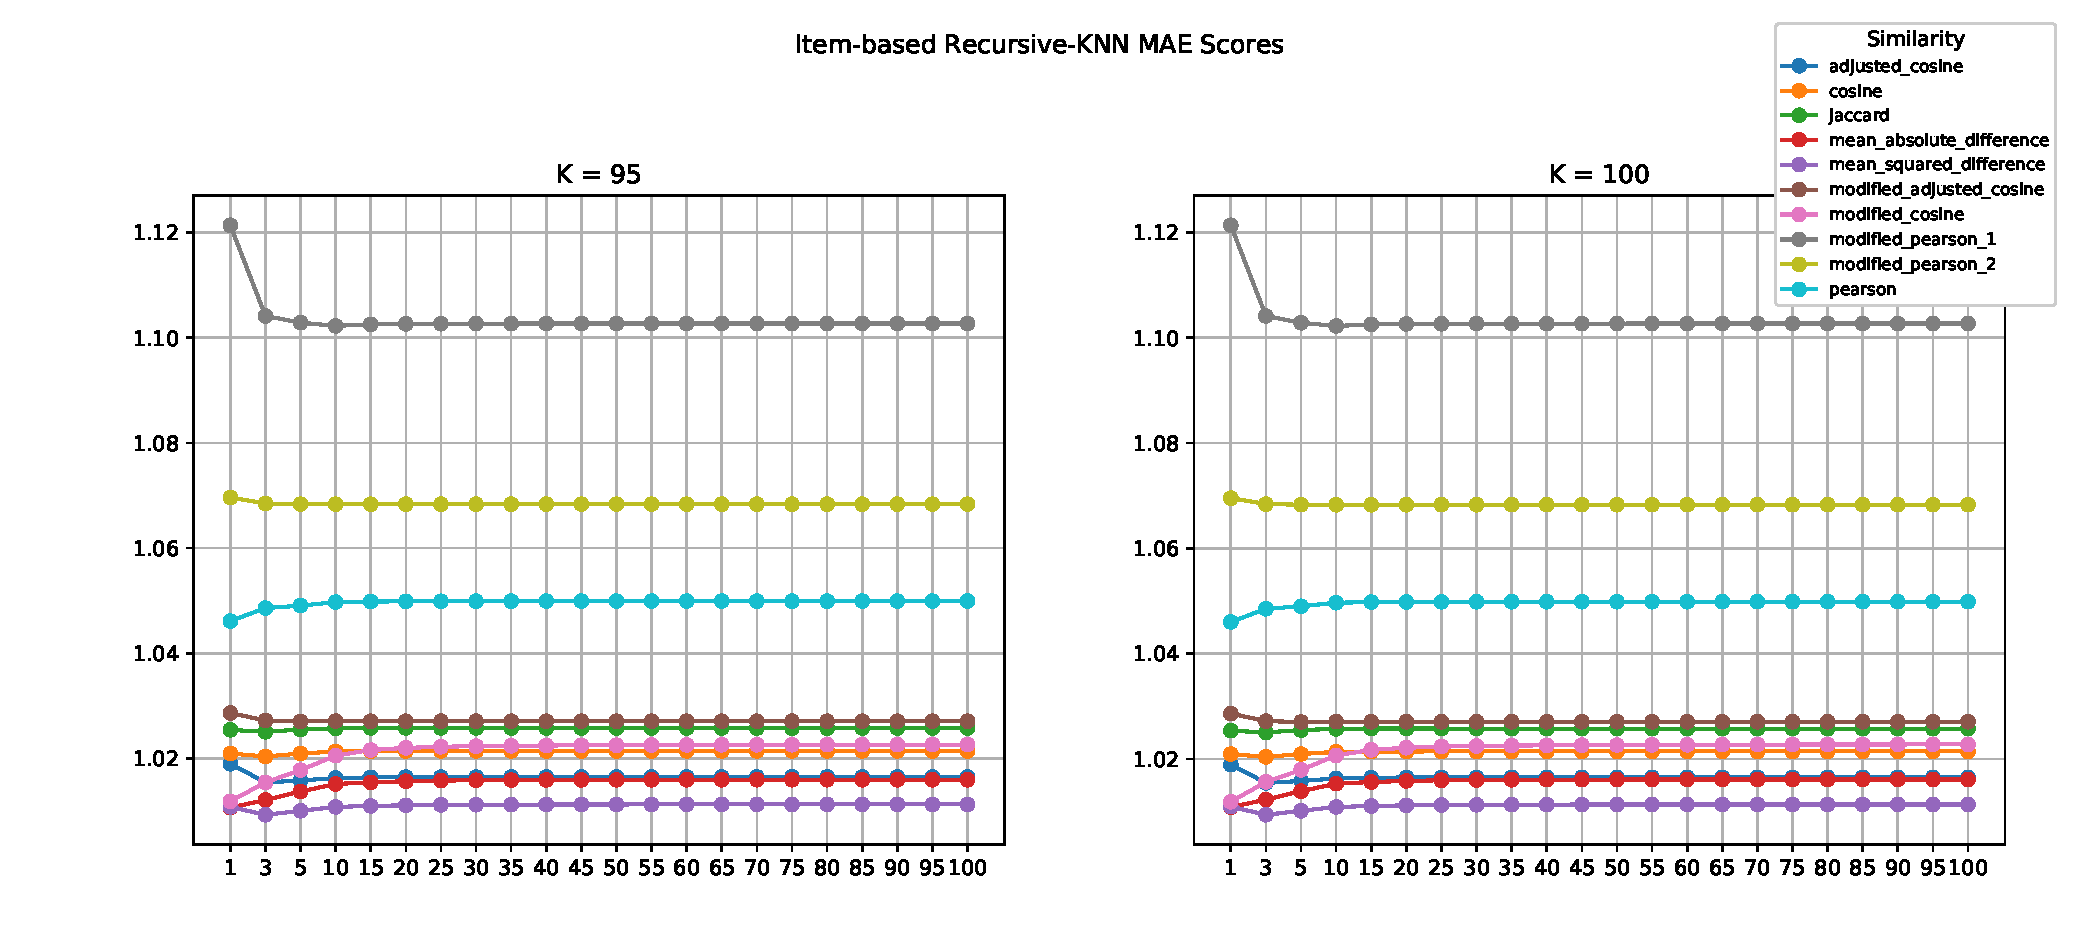
\includegraphics[width=1\textwidth]{chapter_4/rknn/mae/item_95_100.eps}
\caption{Item-based RKNN MAE scores}
\end{figure}

\subsubsection{User-Based}

\begin{figure}[H]
\centering
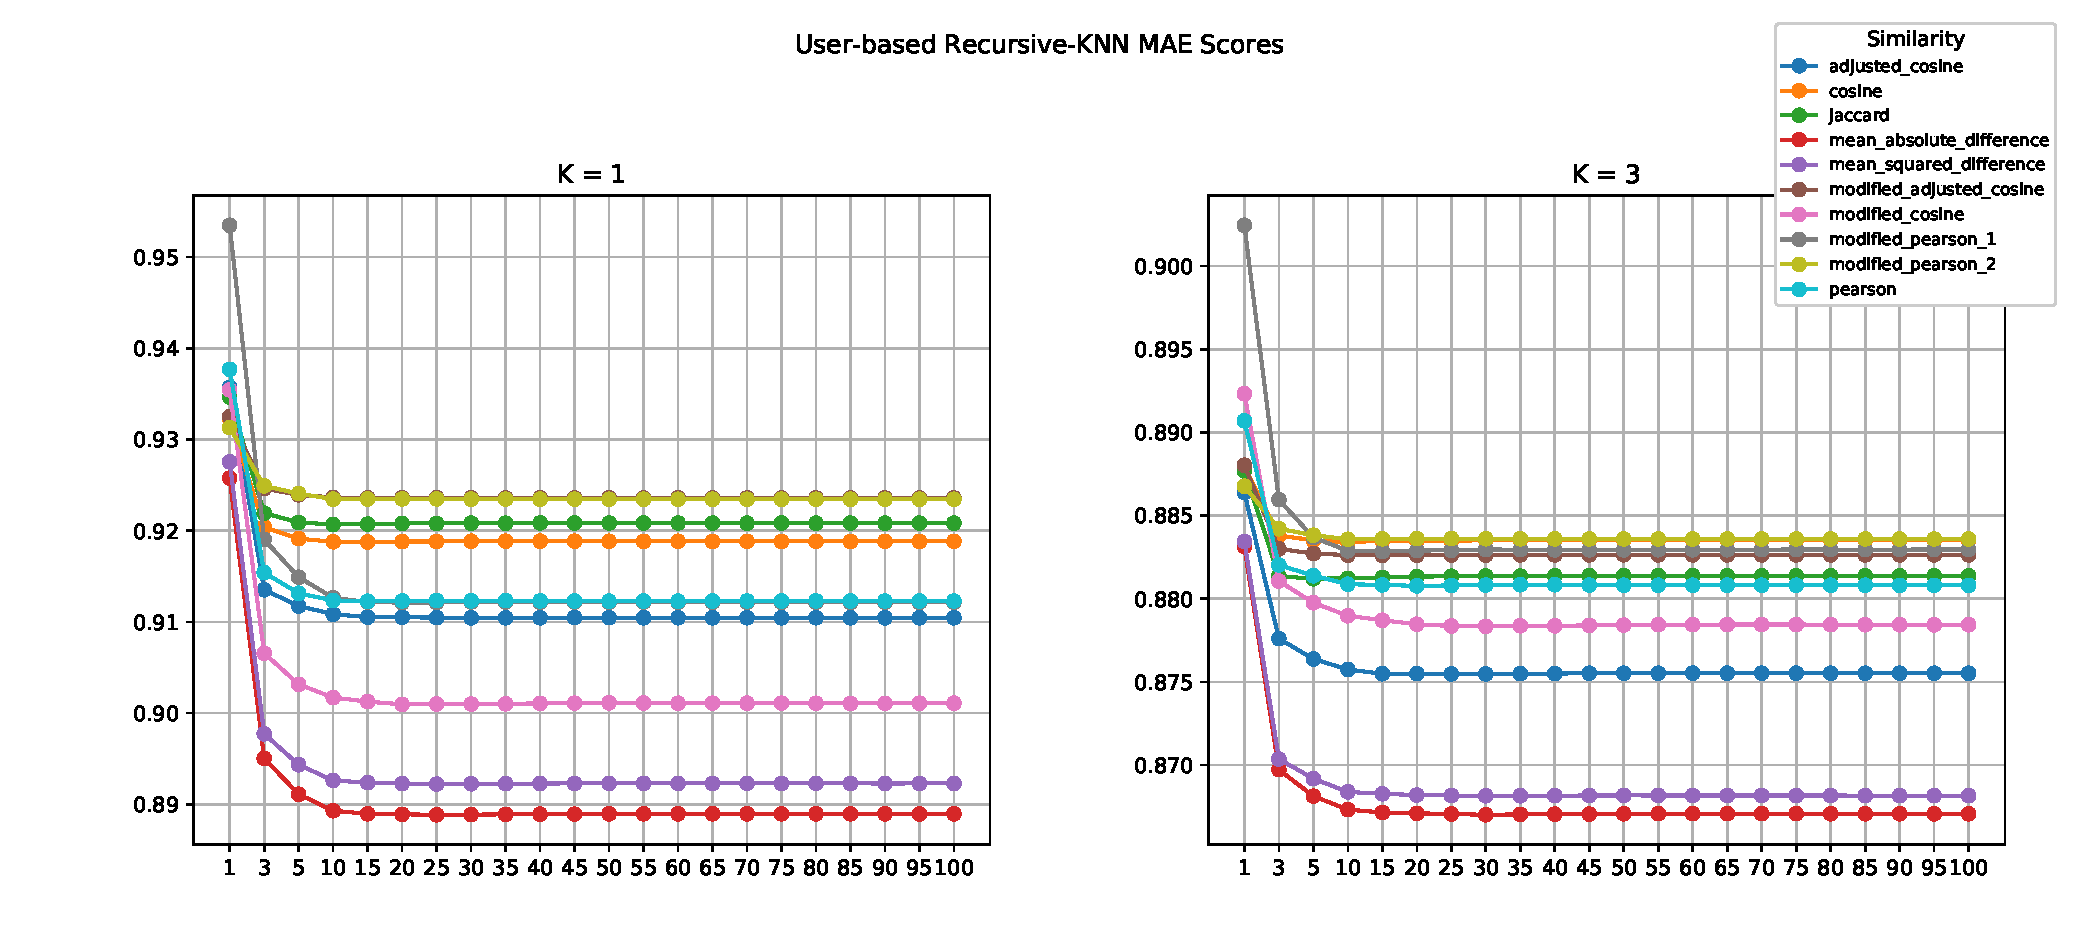
\includegraphics[width=1\textwidth]{chapter_4/rknn/mae/user_1_3.eps}
\caption{User-based RKNN MAE scores}
\end{figure}

\begin{figure}[H]
\centering
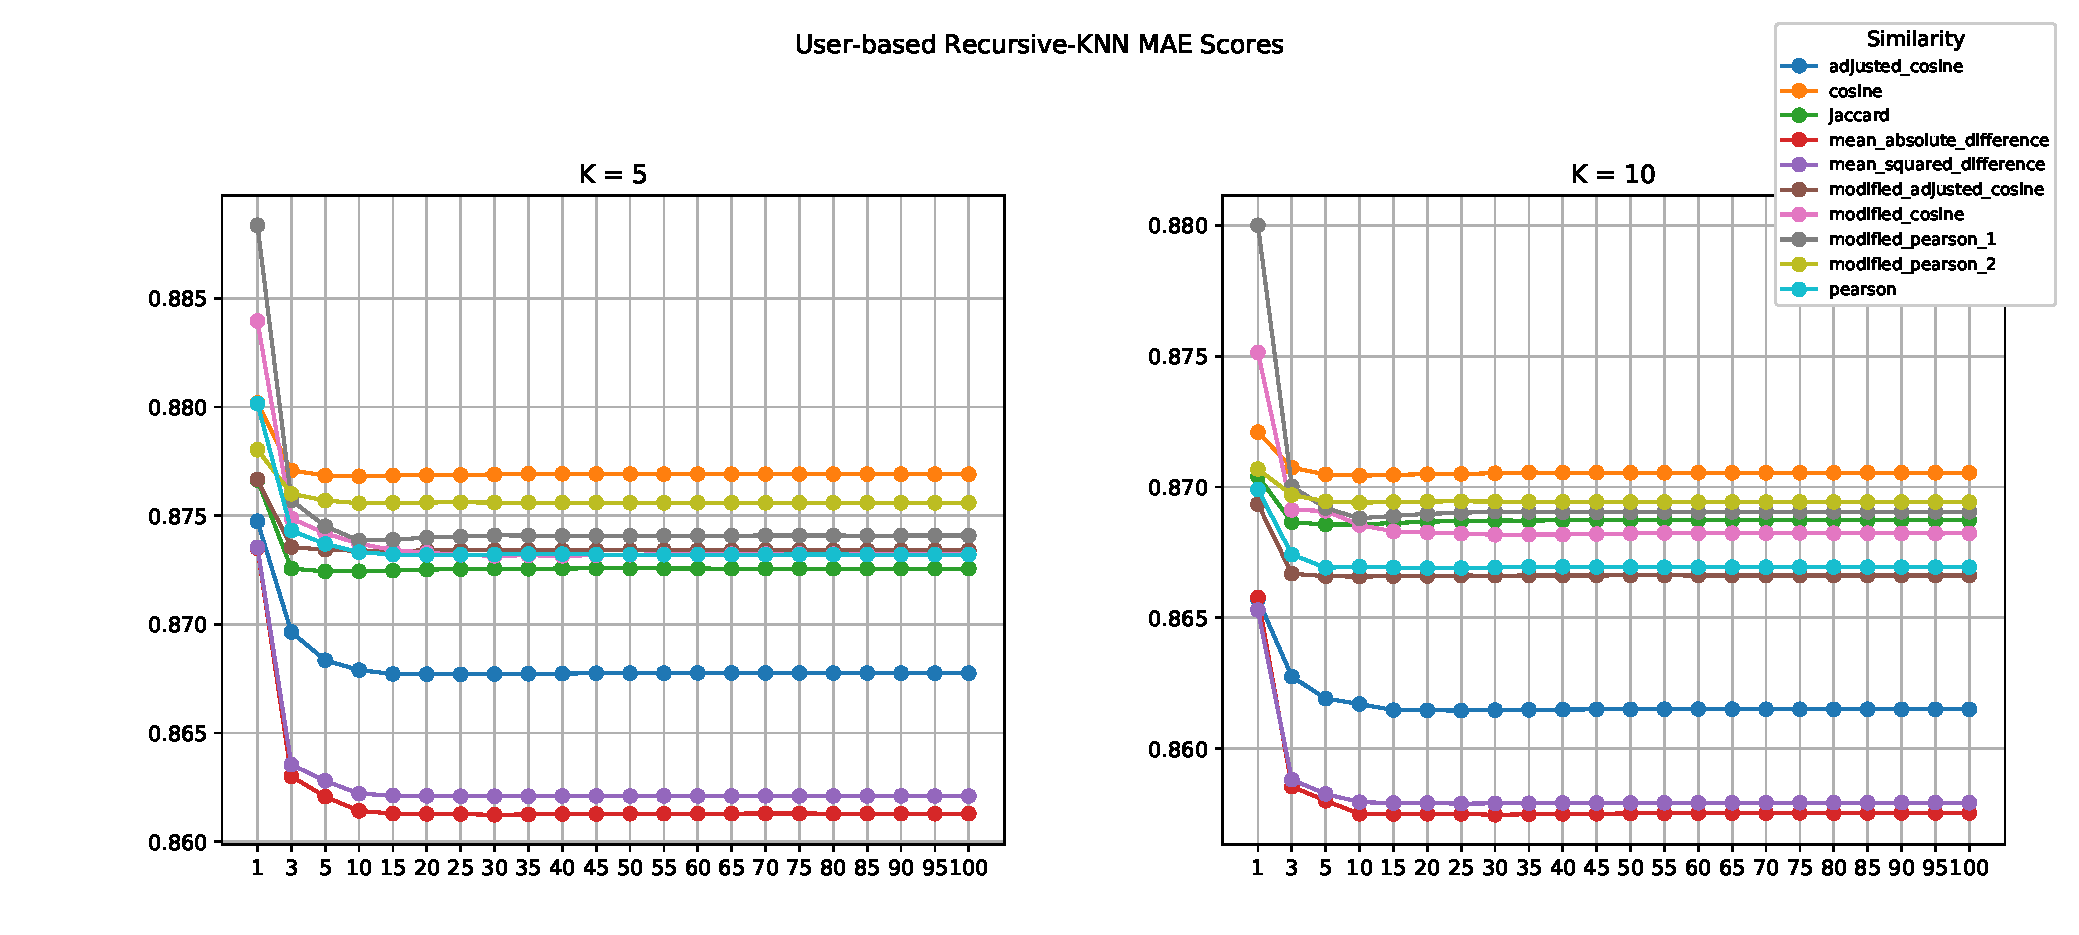
\includegraphics[width=1\textwidth]{chapter_4/rknn/mae/user_5_10.eps}
\caption{User-based RKNN MAE scores}
\end{figure}

\begin{figure}[H]
\centering
\includegraphics[width=1\textwidth]{chapter_4/rknn/mae/user_15_20.eps}
\caption{User-based RKNN MAE scores}
\end{figure}

\begin{figure}[H]
\centering
\includegraphics[width=1\textwidth]{chapter_4/rknn/mae/user_25_30.eps}
\caption{User-based RKNN MAE scores}
\end{figure}

\begin{figure}[H]
\centering
\includegraphics[width=1\textwidth]{chapter_4/rknn/mae/user_35_40.eps}
\caption{User-based RKNN MAE scores}
\end{figure}

\begin{figure}[H]
\centering
\includegraphics[width=1\textwidth]{chapter_4/rknn/mae/user_45_50.eps}
\caption{User-based RKNN MAE scores}
\end{figure}

\begin{figure}[H]
\centering
\includegraphics[width=1\textwidth]{chapter_4/rknn/mae/user_55_60.eps}
\caption{User-based RKNN MAE scores}
\end{figure}

\begin{figure}[H]
\centering
\includegraphics[width=1\textwidth]{chapter_4/rknn/mae/user_65_70.eps}
\caption{User-based RKNN MAE scores}
\end{figure}

\begin{figure}[H]
\centering
\includegraphics[width=1\textwidth]{chapter_4/rknn/mae/user_75_80.eps}
\caption{User-based RKNN MAE scores}
\end{figure}

\begin{figure}[H]
\centering
\includegraphics[width=1\textwidth]{chapter_4/rknn/mae/user_85_90.eps}
\caption{User-based RKNN MAE scores}
\end{figure}

\begin{figure}[H]
\centering
\includegraphics[width=1\textwidth]{chapter_4/rknn/mae/user_95_100.eps}
\caption{User-based RKNN MAE scores}
\end{figure}

\subsection{RMSE}

\subsubsection{Item-Based}

\begin{figure}[H]
\centering
\includegraphics[width=1\textwidth]{chapter_4/rknn/rmse/item_1_3.eps}
\caption{Item-based RKNN RMSE scores}
\end{figure}

\begin{figure}[H]
\centering
\includegraphics[width=1\textwidth]{chapter_4/rknn/rmse/item_5_10.eps}
\caption{Item-based RKNN RMSE scores}
\end{figure}

\begin{figure}[H]
\centering
\includegraphics[width=1\textwidth]{chapter_4/rknn/rmse/item_15_20.eps}
\caption{Item-based RKNN RMSE scores}
\end{figure}

\begin{figure}[H]
\centering
\includegraphics[width=1\textwidth]{chapter_4/rknn/rmse/item_25_30.eps}
\caption{Item-based RKNN RMSE scores}
\end{figure}

\begin{figure}[H]
\centering
\includegraphics[width=1\textwidth]{chapter_4/rknn/rmse/item_35_40.eps}
\caption{Item-based RKNN RMSE scores}
\end{figure}

\begin{figure}[H]
\centering
\includegraphics[width=1\textwidth]{chapter_4/rknn/rmse/item_45_50.eps}
\caption{Item-based RKNN RMSE scores}
\end{figure}

\begin{figure}[H]
\centering
\includegraphics[width=1\textwidth]{chapter_4/rknn/rmse/item_55_60.eps}
\caption{Item-based RKNN RMSE scores}
\end{figure}

\begin{figure}[H]
\centering
\includegraphics[width=1\textwidth]{chapter_4/rknn/rmse/item_65_70.eps}
\caption{Item-based RKNN RMSE scores}
\end{figure}

\begin{figure}[H]
\centering
\includegraphics[width=1\textwidth]{chapter_4/rknn/rmse/item_75_80.eps}
\caption{Item-based RKNN RMSE scores}
\end{figure}

\begin{figure}[H]
\centering
\includegraphics[width=1\textwidth]{chapter_4/rknn/rmse/item_85_90.eps}
\caption{Item-based RKNN RMSE scores}
\end{figure}

\begin{figure}[H]
\centering
\includegraphics[width=1\textwidth]{chapter_4/rknn/rmse/item_95_100.eps}
\caption{Item-based RKNN RMSE scores}
\end{figure}

\subsubsection{User-Based}

\begin{figure}[H]
\centering
\includegraphics[width=1\textwidth]{chapter_4/rknn/rmse/user_1_3.eps}
\caption{User-based RKNN RMSE scores}
\end{figure}

\begin{figure}[H]
\centering
\includegraphics[width=1\textwidth]{chapter_4/rknn/rmse/user_5_10.eps}
\caption{User-based RKNN RMSE scores}
\end{figure}

\begin{figure}[H]
\centering
\includegraphics[width=1\textwidth]{chapter_4/rknn/rmse/user_15_20.eps}
\caption{User-based RKNN RMSE scores}
\end{figure}

\begin{figure}[H]
\centering
\includegraphics[width=1\textwidth]{chapter_4/rknn/rmse/user_25_30.eps}
\caption{User-based RKNN RMSE scores}
\end{figure}

\begin{figure}[H]
\centering
\includegraphics[width=1\textwidth]{chapter_4/rknn/rmse/user_35_40.eps}
\caption{User-based RKNN RMSE scores}
\end{figure}

\begin{figure}[H]
\centering
\includegraphics[width=1\textwidth]{chapter_4/rknn/rmse/user_45_50.eps}
\caption{User-based RKNN RMSE scores}
\end{figure}

\begin{figure}[H]
\centering
\includegraphics[width=1\textwidth]{chapter_4/rknn/rmse/user_55_60.eps}
\caption{User-based RKNN RMSE scores}
\end{figure}

\begin{figure}[H]
\centering
\includegraphics[width=1\textwidth]{chapter_4/rknn/rmse/user_65_70.eps}
\caption{User-based RKNN RMSE scores}
\end{figure}

\begin{figure}[H]
\centering
\includegraphics[width=1\textwidth]{chapter_4/rknn/rmse/user_75_80.eps}
\caption{User-based RKNN RMSE scores}
\end{figure}

\begin{figure}[H]
\centering
\includegraphics[width=1\textwidth]{chapter_4/rknn/rmse/user_85_90.eps}
\caption{User-based RKNN RMSE scores}
\end{figure}

\begin{figure}[H]
\centering
\includegraphics[width=1\textwidth]{chapter_4/rknn/rmse/user_95_100.eps}
\caption{User-based RKNN RMSE scores}
\end{figure}

\subsection{MAUE}

\subsubsection{Item-Based}

\begin{figure}[H]
\centering
\includegraphics[width=1\textwidth]{chapter_4/rknn/maue/item_1_3.eps}
\caption{Item-based RKNN MAUE scores}
\end{figure}

\begin{figure}[H]
\centering
\includegraphics[width=1\textwidth]{chapter_4/rknn/maue/item_5_10.eps}
\caption{Item-based RKNN MAUE scores}
\end{figure}

\begin{figure}[H]
\centering
\includegraphics[width=1\textwidth]{chapter_4/rknn/maue/item_15_20.eps}
\caption{Item-based RKNN MAUE scores}
\end{figure}

\begin{figure}[H]
\centering
\includegraphics[width=1\textwidth]{chapter_4/rknn/maue/item_25_30.eps}
\caption{Item-based RKNN MAUE scores}
\end{figure}

\begin{figure}[H]
\centering
\includegraphics[width=1\textwidth]{chapter_4/rknn/maue/item_35_40.eps}
\caption{Item-based RKNN MAUE scores}
\end{figure}

\begin{figure}[H]
\centering
\includegraphics[width=1\textwidth]{chapter_4/rknn/maue/item_45_50.eps}
\caption{Item-based RKNN MAUE scores}
\end{figure}

\begin{figure}[H]
\centering
\includegraphics[width=1\textwidth]{chapter_4/rknn/maue/item_55_60.eps}
\caption{Item-based RKNN MAUE scores}
\end{figure}

\begin{figure}[H]
\centering
\includegraphics[width=1\textwidth]{chapter_4/rknn/maue/item_65_70.eps}
\caption{Item-based RKNN MAUE scores}
\end{figure}

\begin{figure}[H]
\centering
\includegraphics[width=1\textwidth]{chapter_4/rknn/maue/item_75_80.eps}
\caption{Item-based RKNN MAUE scores}
\end{figure}

\begin{figure}[H]
\centering
\includegraphics[width=1\textwidth]{chapter_4/rknn/maue/item_85_90.eps}
\caption{Item-based RKNN MAUE scores}
\end{figure}

\begin{figure}[H]
\centering
\includegraphics[width=1\textwidth]{chapter_4/rknn/maue/item_95_100.eps}
\caption{Item-based RKNN MAUE scores}
\end{figure}

\subsubsection{User-Based}

\begin{figure}[H]
\centering
\includegraphics[width=1\textwidth]{chapter_4/rknn/maue/user_1_3.eps}
\caption{User-based RKNN MAUE scores}
\end{figure}

\begin{figure}[H]
\centering
\includegraphics[width=1\textwidth]{chapter_4/rknn/maue/user_5_10.eps}
\caption{User-based RKNN MAUE scores}
\end{figure}

\begin{figure}[H]
\centering
\includegraphics[width=1\textwidth]{chapter_4/rknn/maue/user_15_20.eps}
\caption{User-based RKNN MAUE scores}
\end{figure}

\begin{figure}[H]
\centering
\includegraphics[width=1\textwidth]{chapter_4/rknn/maue/user_25_30.eps}
\caption{User-based RKNN MAUE scores}
\end{figure}

\begin{figure}[H]
\centering
\includegraphics[width=1\textwidth]{chapter_4/rknn/maue/user_35_40.eps}
\caption{User-based RKNN MAUE scores}
\end{figure}

\begin{figure}[H]
\centering
\includegraphics[width=1\textwidth]{chapter_4/rknn/maue/user_45_50.eps}
\caption{User-based RKNN MAUE scores}
\end{figure}

\begin{figure}[H]
\centering
\includegraphics[width=1\textwidth]{chapter_4/rknn/maue/user_55_60.eps}
\caption{User-based RKNN MAUE scores}
\end{figure}

\begin{figure}[H]
\centering
\includegraphics[width=1\textwidth]{chapter_4/rknn/maue/user_65_70.eps}
\caption{User-based RKNN MAUE scores}
\end{figure}

\begin{figure}[H]
\centering
\includegraphics[width=1\textwidth]{chapter_4/rknn/maue/user_75_80.eps}
\caption{User-based RKNN MAUE scores}
\end{figure}

\begin{figure}[H]
\centering
\includegraphics[width=1\textwidth]{chapter_4/rknn/maue/user_85_90.eps}
\caption{User-based RKNN MAUE scores}
\end{figure}

\begin{figure}[H]
\centering
\includegraphics[width=1\textwidth]{chapter_4/rknn/maue/user_95_100.eps}
\caption{User-based RKNN MAUE scores}
\end{figure}

\subsection{RMSUE}

\subsubsection{Item-Based}

\begin{figure}[H]
\centering
\includegraphics[width=1\textwidth]{chapter_4/rknn/rmsue/item_1_3.eps}
\caption{Item-based RKNN RMSUE scores}
\end{figure}

\begin{figure}[H]
\centering
\includegraphics[width=1\textwidth]{chapter_4/rknn/rmsue/item_5_10.eps}
\caption{Item-based RKNN RMSUE scores}
\end{figure}

\begin{figure}[H]
\centering
\includegraphics[width=1\textwidth]{chapter_4/rknn/rmsue/item_15_20.eps}
\caption{Item-based RKNN RMSUE scores}
\end{figure}

\begin{figure}[H]
\centering
\includegraphics[width=1\textwidth]{chapter_4/rknn/rmsue/item_25_30.eps}
\caption{Item-based RKNN RMSUE scores}
\end{figure}

\begin{figure}[H]
\centering
\includegraphics[width=1\textwidth]{chapter_4/rknn/rmsue/item_35_40.eps}
\caption{Item-based RKNN RMSUE scores}
\end{figure}

\begin{figure}[H]
\centering
\includegraphics[width=1\textwidth]{chapter_4/rknn/rmsue/item_45_50.eps}
\caption{Item-based RKNN RMSUE scores}
\end{figure}

\begin{figure}[H]
\centering
\includegraphics[width=1\textwidth]{chapter_4/rknn/rmsue/item_55_60.eps}
\caption{Item-based RKNN RMSUE scores}
\end{figure}

\begin{figure}[H]
\centering
\includegraphics[width=1\textwidth]{chapter_4/rknn/rmsue/item_65_70.eps}
\caption{Item-based RKNN RMSUE scores}
\end{figure}

\begin{figure}[H]
\centering
\includegraphics[width=1\textwidth]{chapter_4/rknn/rmsue/item_75_80.eps}
\caption{Item-based RKNN RMSUE scores}
\end{figure}

\begin{figure}[H]
\centering
\includegraphics[width=1\textwidth]{chapter_4/rknn/rmsue/item_85_90.eps}
\caption{Item-based RKNN RMSUE scores}
\end{figure}

\begin{figure}[H]
\centering
\includegraphics[width=1\textwidth]{chapter_4/rknn/rmsue/item_95_100.eps}
\caption{Item-based RKNN RMSUE scores}
\end{figure}

\subsubsection{User-Based}

\begin{figure}[H]
\centering
\includegraphics[width=1\textwidth]{chapter_4/rknn/rmsue/user_1_3.eps}
\caption{User-based RKNN RMSUE scores}
\end{figure}

\begin{figure}[H]
\centering
\includegraphics[width=1\textwidth]{chapter_4/rknn/rmsue/user_5_10.eps}
\caption{User-based RKNN RMSUE scores}
\end{figure}

\begin{figure}[H]
\centering
\includegraphics[width=1\textwidth]{chapter_4/rknn/rmsue/user_15_20.eps}
\caption{User-based RKNN RMSUE scores}
\end{figure}

\begin{figure}[H]
\centering
\includegraphics[width=1\textwidth]{chapter_4/rknn/rmsue/user_25_30.eps}
\caption{User-based RKNN RMSUE scores}
\end{figure}

\begin{figure}[H]
\centering
\includegraphics[width=1\textwidth]{chapter_4/rknn/rmsue/user_35_40.eps}
\caption{User-based RKNN RMSUE scores}
\end{figure}

\begin{figure}[H]
\centering
\includegraphics[width=1\textwidth]{chapter_4/rknn/rmsue/user_45_50.eps}
\caption{User-based RKNN RMSUE scores}
\end{figure}

\begin{figure}[H]
\centering
\includegraphics[width=1\textwidth]{chapter_4/rknn/rmsue/user_55_60.eps}
\caption{User-based RKNN RMSUE scores}
\end{figure}

\begin{figure}[H]
\centering
\includegraphics[width=1\textwidth]{chapter_4/rknn/rmsue/user_65_70.eps}
\caption{User-based RKNN RMSUE scores}
\end{figure}

\begin{figure}[H]
\centering
\includegraphics[width=1\textwidth]{chapter_4/rknn/rmsue/user_75_80.eps}
\caption{User-based RKNN RMSUE scores}
\end{figure}

\begin{figure}[H]
\centering
\includegraphics[width=1\textwidth]{chapter_4/rknn/rmsue/user_85_90.eps}
\caption{User-based RKNN RMSUE scores}
\end{figure}

\begin{figure}[H]
\centering
\includegraphics[width=1\textwidth]{chapter_4/rknn/rmsue/user_95_100.eps}
\caption{User-based RKNN RMSUE scores}
\end{figure}

\section{Total Scores}

\subsection{MAE}

\subsubsection{Item-Based}

\begin{figure}[H]
\centering
\includegraphics[width=1\textwidth]{chapter_4/total/mae/item_1_3.eps}
\caption{Item-based Total MAE scores}
\end{figure}

\begin{figure}[H]
\centering
\includegraphics[width=1\textwidth]{chapter_4/total/mae/item_5_10.eps}
\caption{Item-based Total MAE scores}
\end{figure}

\begin{figure}[H]
\centering
\includegraphics[width=1\textwidth]{chapter_4/total/mae/item_15_20.eps}
\caption{Item-based Total MAE scores}
\end{figure}

\begin{figure}[H]
\centering
\includegraphics[width=1\textwidth]{chapter_4/total/mae/item_25_30.eps}
\caption{Item-based Total MAE scores}
\end{figure}

\begin{figure}[H]
\centering
\includegraphics[width=1\textwidth]{chapter_4/total/mae/item_35_40.eps}
\caption{Item-based Total MAE scores}
\end{figure}

\begin{figure}[H]
\centering
\includegraphics[width=1\textwidth]{chapter_4/total/mae/item_45_50.eps}
\caption{Item-based Total MAE scores}
\end{figure}

\begin{figure}[H]
\centering
\includegraphics[width=1\textwidth]{chapter_4/total/mae/item_55_60.eps}
\caption{Item-based Total MAE scores}
\end{figure}

\begin{figure}[H]
\centering
\includegraphics[width=1\textwidth]{chapter_4/total/mae/item_65_70.eps}
\caption{Item-based Total MAE scores}
\end{figure}

\begin{figure}[H]
\centering
\includegraphics[width=1\textwidth]{chapter_4/total/mae/item_75_80.eps}
\caption{Item-based Total MAE scores}
\end{figure}

\begin{figure}[H]
\centering
\includegraphics[width=1\textwidth]{chapter_4/total/mae/item_85_90.eps}
\caption{Item-based Total MAE scores}
\end{figure}

\begin{figure}[H]
\centering
\includegraphics[width=1\textwidth]{chapter_4/total/mae/item_95_100.eps}
\caption{Item-based Total MAE scores}
\end{figure}

\subsubsection{User-Based}

\begin{figure}[H]
\centering
\includegraphics[width=1\textwidth]{chapter_4/total/mae/user_1_3.eps}
\caption{User-based Total MAE scores}
\end{figure}

\begin{figure}[H]
\centering
\includegraphics[width=1\textwidth]{chapter_4/total/mae/user_5_10.eps}
\caption{User-based Total MAE scores}
\end{figure}

\begin{figure}[H]
\centering
\includegraphics[width=1\textwidth]{chapter_4/total/mae/user_15_20.eps}
\caption{User-based Total MAE scores}
\end{figure}

\begin{figure}[H]
\centering
\includegraphics[width=1\textwidth]{chapter_4/total/mae/user_25_30.eps}
\caption{User-based Total MAE scores}
\end{figure}

\begin{figure}[H]
\centering
\includegraphics[width=1\textwidth]{chapter_4/total/mae/user_35_40.eps}
\caption{User-based Total MAE scores}
\end{figure}

\begin{figure}[H]
\centering
\includegraphics[width=1\textwidth]{chapter_4/total/mae/user_45_50.eps}
\caption{User-based Total MAE scores}
\end{figure}

\begin{figure}[H]
\centering
\includegraphics[width=1\textwidth]{chapter_4/total/mae/user_55_60.eps}
\caption{User-based Total MAE scores}
\end{figure}

\begin{figure}[H]
\centering
\includegraphics[width=1\textwidth]{chapter_4/total/mae/user_65_70.eps}
\caption{User-based Total MAE scores}
\end{figure}

\begin{figure}[H]
\centering
\includegraphics[width=1\textwidth]{chapter_4/total/mae/user_75_80.eps}
\caption{User-based Total MAE scores}
\end{figure}

\begin{figure}[H]
\centering
\includegraphics[width=1\textwidth]{chapter_4/total/mae/user_85_90.eps}
\caption{User-based Total MAE scores}
\end{figure}

\begin{figure}[H]
\centering
\includegraphics[width=1\textwidth]{chapter_4/total/mae/user_95_100.eps}
\caption{User-based Total MAE scores}
\end{figure}

\subsection{RMSE}

\subsubsection{Item-Based}

\begin{figure}[H]
\centering
\includegraphics[width=1\textwidth]{chapter_4/total/rmse/item_1_3.eps}
\caption{Item-based Total RMSE scores}
\end{figure}

\begin{figure}[H]
\centering
\includegraphics[width=1\textwidth]{chapter_4/total/rmse/item_5_10.eps}
\caption{Item-based Total RMSE scores}
\end{figure}

\begin{figure}[H]
\centering
\includegraphics[width=1\textwidth]{chapter_4/total/rmse/item_15_20.eps}
\caption{Item-based Total RMSE scores}
\end{figure}

\begin{figure}[H]
\centering
\includegraphics[width=1\textwidth]{chapter_4/total/rmse/item_25_30.eps}
\caption{Item-based Total RMSE scores}
\end{figure}

\begin{figure}[H]
\centering
\includegraphics[width=1\textwidth]{chapter_4/total/rmse/item_35_40.eps}
\caption{Item-based Total RMSE scores}
\end{figure}

\begin{figure}[H]
\centering
\includegraphics[width=1\textwidth]{chapter_4/total/rmse/item_45_50.eps}
\caption{Item-based Total RMSE scores}
\end{figure}

\begin{figure}[H]
\centering
\includegraphics[width=1\textwidth]{chapter_4/total/rmse/item_55_60.eps}
\caption{Item-based Total RMSE scores}
\end{figure}

\begin{figure}[H]
\centering
\includegraphics[width=1\textwidth]{chapter_4/total/rmse/item_65_70.eps}
\caption{Item-based Total RMSE scores}
\end{figure}

\begin{figure}[H]
\centering
\includegraphics[width=1\textwidth]{chapter_4/total/rmse/item_75_80.eps}
\caption{Item-based Total RMSE scores}
\end{figure}

\begin{figure}[H]
\centering
\includegraphics[width=1\textwidth]{chapter_4/total/rmse/item_85_90.eps}
\caption{Item-based Total RMSE scores}
\end{figure}

\begin{figure}[H]
\centering
\includegraphics[width=1\textwidth]{chapter_4/total/rmse/item_95_100.eps}
\caption{Item-based Total RMSE scores}
\end{figure}

\subsubsection{User-Based}

\begin{figure}[H]
\centering
\includegraphics[width=1\textwidth]{chapter_4/total/rmse/user_1_3.eps}
\caption{User-based Total RMSE scores}
\end{figure}

\begin{figure}[H]
\centering
\includegraphics[width=1\textwidth]{chapter_4/total/rmse/user_5_10.eps}
\caption{User-based Total RMSE scores}
\end{figure}

\begin{figure}[H]
\centering
\includegraphics[width=1\textwidth]{chapter_4/total/rmse/user_15_20.eps}
\caption{User-based Total RMSE scores}
\end{figure}

\begin{figure}[H]
\centering
\includegraphics[width=1\textwidth]{chapter_4/total/rmse/user_25_30.eps}
\caption{User-based Total RMSE scores}
\end{figure}

\begin{figure}[H]
\centering
\includegraphics[width=1\textwidth]{chapter_4/total/rmse/user_35_40.eps}
\caption{User-based Total RMSE scores}
\end{figure}

\begin{figure}[H]
\centering
\includegraphics[width=1\textwidth]{chapter_4/total/rmse/user_45_50.eps}
\caption{User-based Total RMSE scores}
\end{figure}

\begin{figure}[H]
\centering
\includegraphics[width=1\textwidth]{chapter_4/total/rmse/user_55_60.eps}
\caption{User-based Total RMSE scores}
\end{figure}

\begin{figure}[H]
\centering
\includegraphics[width=1\textwidth]{chapter_4/total/rmse/user_65_70.eps}
\caption{User-based Total RMSE scores}
\end{figure}

\begin{figure}[H]
\centering
\includegraphics[width=1\textwidth]{chapter_4/total/rmse/user_75_80.eps}
\caption{User-based Total RMSE scores}
\end{figure}

\begin{figure}[H]
\centering
\includegraphics[width=1\textwidth]{chapter_4/total/rmse/user_85_90.eps}
\caption{User-based Total RMSE scores}
\end{figure}

\begin{figure}[H]
\centering
\includegraphics[width=1\textwidth]{chapter_4/total/rmse/user_95_100.eps}
\caption{User-based Total RMSE scores}
\end{figure}

\end{document}
